%==============================================================================
% Tento soubor použijte jako základ
% This file should be used as a base for the thesis
% Autoři / Authors: 2008 Michal Bidlo, 2022 Jaroslav Dytrych
% Kontakt pro dotazy a připomínky: sablona@fit.vutbr.cz
% Contact for questions and comments: sablona@fit.vutbr.cz
%==============================================================================
% kódování: UTF-8 (zmena prikazem iconv, recode nebo cstocs)
% encoding: UTF-8 (you can change it by command iconv, recode or cstocs)
%------------------------------------------------------------------------------
% zpracování / processing: make, make pdf, make clean
%==============================================================================
% Soubory, které je nutné upravit nebo smazat: / Files which have to be edited or deleted:
%   xmacko13-Kontrola-diplomovych-praci-20-literatura-bibliography.bib - literatura / bibliography
%   xmacko13-Kontrola-diplomovych-praci-01-kapitoly-chapters.tex - obsah práce / the thesis content
%   xmacko13-Kontrola-diplomovych-praci-01-kapitoly-chapters-en.tex - obsah práce v angličtině / the thesis content in English
%   xmacko13-Kontrola-diplomovych-praci-30-prilohy-appendices.tex - přílohy / appendices
%   xmacko13-Kontrola-diplomovych-praci-30-prilohy-appendices-en.tex - přílohy v angličtině / appendices in English
%==============================================================================
\documentclass[]{fitthesis} % bez zadání - pro začátek práce, aby nebyl problém s překladem
%\documentclass[english]{fitthesis} % without assignment - for the work start to avoid compilation problem
%\documentclass[zadani]{fitthesis} % odevzdani do IS VUT a/nebo tisk s barevnými odkazy - odkazy jsou barevné
%\documentclass[english,zadani]{fitthesis} % for submission to the IS VUT and/or print with color links - links are color
%\documentclass[zadani,print]{fitthesis} % pro černobílý tisk - odkazy jsou černé
%\documentclass[english,zadani,print]{fitthesis} % for the black and white print - links are black
%\documentclass[zadani,cprint]{fitthesis} % pro barevný tisk - odkazy jsou černé, znak VUT barevný
%\documentclass[english,zadani,cprint]{fitthesis} % for the print - links are black, logo is color
% * Je-li práce psaná v anglickém jazyce, je zapotřebí u třídy použít 
%   parametr english následovně:
%   If thesis is written in English, it is necessary to use 
%   parameter english as follows:
%      \documentclass[english]{fitthesis}
% * Je-li práce psaná ve slovenském jazyce, je zapotřebí u třídy použít 
%   parametr slovak následovně:
%   If the work is written in the Slovak language, it is necessary 
%   to use parameter slovak as follows:
%      \documentclass[slovak]{fitthesis}
% * Je-li práce psaná v anglickém jazyce se slovenským abstraktem apod., 
%   je zapotřebí u třídy použít parametry english a enslovak následovně:
%   If the work is written in English with the Slovak abstract, etc., 
%   it is necessary to use parameters english and enslovak as follows:
%      \documentclass[english,enslovak]{fitthesis}


% Základní balíčky jsou dole v souboru šablony fitthesis.cls
% Basic packages are at the bottom of template file fitthesis.cls
% zde můžeme vložit vlastní balíčky / you can place own packages here


% Pro seznam zkratek lze využít balíček Glossaries - nutno odkomentovat i níže a při kompilaci z konzoly i v Makefile (plnou verzi pro Perl, nebo lite)
% The Glossaries package can be used for the list of abbreviations - it is necessary to uncomment also below. When compiling from the console also in the Makefile (full version for Perl or lite)
%\usepackage{glossaries}
%\usepackage{glossary-superragged}
%\makeglossaries 

% Nastavení cesty k obrázkům
% Setting of a path to the pictures
%\graphicspath{{obrazky-figures/}{./obrazky-figures/}}
%\graphicspath{{obrazky-figures/}{../obrazky-figures/}}

%---rm---------------
\renewcommand{\rmdefault}{lmr}%zavede Latin Modern Roman jako rm / set Latin Modern Roman as rm
%---sf---------------
\renewcommand{\sfdefault}{qhv}%zavede TeX Gyre Heros jako sf
%---tt------------
\renewcommand{\ttdefault}{lmtt}% zavede Latin Modern tt jako tt

% vypne funkci šablony, která automaticky nahrazuje uvozovky,
% aby nebyly prováděny nevhodné náhrady v popisech API apod.
% disables function of the template which replaces quotation marks
% to avoid unnecessary replacements in the API descriptions etc.
\csdoublequotesoff

\usepackage{url}
\usepackage{xcolor}
\newcommand{\dummyText}[1][1]{{\color{lightgray}\blindtext[#1]}}
\newcommand{\DummyText}[0]{{\color{lightgray}\Blindtext}}
\usepackage{pgffor}
\newcommand{\blindshort}[1][3]{
  \def\loremtext{
    {Lorem ipsum dolor sit amet, consectetuer adipiscing elit.},
    {Etiam lobortis facilisis sem.},
    {Nullam nec mi et neque pharetra sollicitudin.},
    {Praesent imperdiet mi nec ante.},
    {Donec ullamcorper, felis non sodales commodo, lectus velit ultrices augue, a dignissim nibh lectus placerat pede.},
    {Vivamus nunc nunc, molestie ut, ultricies vel, semper in, velit.},
    {Ut porttitor.},
    {Praesent in sapien.},
    {Lorem ipsum dolor sit amet, consectetuer adipiscing elit.},
    {Duis fringilla tristique neque.},
    {Sed interdum libero ut metus.},
    {Pellentesque placerat.},
    {Nam rutrum augue a leo.},
    {Morbi sed elit sit amet ante lobortis sollicitudin.},
    {Praesent blandit blandit mauris.},
    {Praesent lectus tellus, aliquet aliquam, luctus a, egestas a, turpis.},
    {Mauris lacinia lorem sit amet ipsum.},
    {Nunc quis urna dictum turpis accumsan semper.}}%
  \foreach \texti [count=\i] in \loremtext {
    \ifnum\i>#1
    \else
    \texti
    \fi
  }
}
\newcommand{\dummyShortText}[1][3]{{\color{lightgray}\blindshort[#1]}}

% =======================================================================
% balíček "hyperref" vytváří klikací odkazy v pdf, pokud tedy použijeme pdflatex
% problém je, že balíček hyperref musí být uveden jako poslední, takže nemůže
% být v šabloně
% "hyperref" package create clickable links in pdf if you are using pdflatex.
% Problem is that this package have to be introduced as the last one so it 
% can not be placed in the template file.
\ifWis
\ifx\pdfoutput\undefined % nejedeme pod pdflatexem / we are not using pdflatex
\else
  \usepackage{color}
  \usepackage[unicode,colorlinks,hyperindex,plainpages=false,pdftex]{hyperref}
  \definecolor{hrcolor-ref}{RGB}{223,52,30}
  \definecolor{hrcolor-cite}{HTML}{2F8F00}
  \definecolor{hrcolor-urls}{HTML}{092EAB}
  \hypersetup{
	linkcolor=hrcolor-ref,
	citecolor=hrcolor-cite,
	filecolor=magenta,
	urlcolor=hrcolor-urls
  }
  \def\pdfBorderAttrs{/Border [0 0 0] }  % bez okrajů kolem odkazů / without margins around links
  \pdfcompresslevel=9
\fi
\else % pro tisk budou odkazy, na které se dá klikat, černé / for the print clickable links will be black
\ifx\pdfoutput\undefined % nejedeme pod pdflatexem / we are not using pdflatex
\else
  \usepackage{color}
  \usepackage[unicode,colorlinks,hyperindex,plainpages=false,pdftex,urlcolor=black,linkcolor=black,citecolor=black]{hyperref}
  \definecolor{links}{rgb}{0,0,0}
  \definecolor{anchors}{rgb}{0,0,0}
  \def\AnchorColor{anchors}
  \def\LinkColor{links}
  \def\pdfBorderAttrs{/Border [0 0 0] } % bez okrajů kolem odkazů / without margins around links
  \pdfcompresslevel=9
\fi
\fi
% Řešení problému, kdy klikací odkazy na obrázky vedou za obrázek
% This solves the problems with links which leads after the picture
\usepackage[all]{hypcap}


% Informace o práci/projektu / Information about the thesis
%---------------------------------------------------------------------------
\projectinfo{
  %Prace / Thesis
  project={BP},            %typ práce BP/SP/DP/DR  / thesis type (SP = term project)
  year={2023},             % rok odevzdání / year of submission
  date=\today,             % datum odevzdání / submission date
  %Nazev prace / thesis title
  title.cs={Nástroj pro kontrolu diplomových prací},  % název práce v češtině či slovenštině (dle zadání) / thesis title in czech language (according to assignment)
  title.en={Theses Checker}, % název práce v angličtině / thesis title in english
  %title.length={14.5cm}, % nastavení délky bloku s titulkem pro úpravu zalomení řádku (lze definovat zde nebo níže) / setting the length of a block with a thesis title for adjusting a line break (can be defined here or below)
  %sectitle.length={14.5cm}, % nastavení délky bloku s druhým titulkem pro úpravu zalomení řádku (lze definovat zde nebo níže) / setting the length of a block with a second thesis title for adjusting a line break (can be defined here or below)
  %dectitle.length={14.5cm}, % nastavení délky bloku s titulkem nad prohlášením pro úpravu zalomení řádku (lze definovat zde nebo níže) / setting the length of a block with a thesis title above declaration for adjusting a line break (can be defined here or below)
  %Autor / Author
  author.name={Michaela},   % jméno autora / author name
  author.surname={Macková},   % příjmení autora / author surname 
  %author.title.p={Bc.}, % titul před jménem (nepovinné) / title before the name (optional)
  %author.title.a={Ph.D.}, % titul za jménem (nepovinné) / title after the name (optional)
  %Ustav / Department
  department={UPGM}, % doplňte příslušnou zkratku dle ústavu na zadání: UPSY/UIFS/UITS/UPGM / fill in appropriate abbreviation of the department according to assignment: UPSY/UIFS/UITS/UPGM
  % Školitel / supervisor
  supervisor.name={Tomáš},   % jméno školitele / supervisor name 
  supervisor.surname={Milet},   % příjmení školitele / supervisor surname
  supervisor.title.p={Ing.},   %titul před jménem (nepovinné) / title before the name (optional)
  supervisor.title.a={Ph.D.},    %titul za jménem (nepovinné) / title after the name (optional)
  % Klíčová slova / keywords
  keywords.cs={Sem budou zapsána jednotlivá klíčová slova v českém (slovenském) jazyce, oddělená čárkami.}, % klíčová slova v českém či slovenském jazyce / keywords in czech or slovak language
  keywords.en={Sem budou zapsána jednotlivá klíčová slova v anglickém jazyce, oddělená čárkami.}, % klíčová slova v anglickém jazyce / keywords in english
  %keywords.en={Here, individual keywords separated by commas will be written in English.},
  % Abstrakt / Abstract
  abstract.cs={Do tohoto odstavce bude zapsán výtah (abstrakt) práce v českém (slovenském) jazyce.}, % abstrakt v českém či slovenském jazyce / abstract in czech or slovak language
  abstract.en={Do tohoto odstavce bude zapsán výtah (abstrakt) práce v anglickém jazyce.}, % abstrakt v anglickém jazyce / abstract in english
  %abstract.en={An abstract of the work in English will be written in this paragraph.},
  % Prohlášení (u anglicky psané práce anglicky, u slovensky psané práce slovensky; u projektové praxe lze zakomentovat) / Declaration (for thesis in english should be in english; for project practice can be commented out)
  declaration={Prohlašuji, že jsem tuto bakalářskou práci vypracoval samostatně pod vedením pana X...
Další informace mi poskytli...
Uvedl jsem všechny literární prameny, publikace a další zdroje, ze kterých jsem čerpal.},
  %declaration={I hereby declare that this Bachelor's thesis was prepared as an original work by the author under the supervision of Mr. X
% The supplementary information was provided by Mr. Y
% I have listed all the literary sources, publications and other sources, which were used during the preparation of this thesis.},
  % Poděkování (nepovinné, nejlépe v jazyce práce; nechcete-li, zakomentujte pro skrytí nadpisu) / Acknowledgement (optional, ideally in the language of the thesis; comment out for hiding including heading)
  acknowledgment={V této sekci je možno uvést poděkování vedoucímu práce a těm, kteří poskytli odbornou pomoc
(externí zadavatel, konzultant apod.).},
  %acknowledgment={Here it is possible to express thanks to the supervisor and to the people which provided professional help
%(external submitter, consultant, etc.).},
  % Rozšířený abstrakt (cca 3 normostrany) - lze definovat zde nebo níže / Extended abstract (approximately 3 standard pages) - can be defined here or below
  %extendedabstract={Do tohoto odstavce bude zapsán rozšířený výtah (abstrakt) práce v českém (slovenském) jazyce.},
  %extabstract.odd={true}, % Začít rozšířený abstrakt na liché stránce? / Should extended abstract start on the odd page?
  %faculty={FIT}, % FIT/FEKT/FSI/FA/FCH/FP/FAST/FAVU/USI/DEF
  faculty.cs={Fakulta informačních technologií}, % Fakulta v češtině - pro využití této položky výše zvolte fakultu DEF / Faculty in Czech - for use of this entry select DEF above
  faculty.en={Faculty of Information Technology}, % Fakulta v angličtině - pro využití této položky výše zvolte fakultu DEF / Faculty in English - for use of this entry select DEF above
  department.cs={Ústav matematiky}, % Ústav v češtině - pro využití této položky výše zvolte ústav DEF nebo jej zakomentujte / Department in Czech - for use of this entry select DEF above or comment it out
  department.en={Institute of Mathematics} % Ústav v angličtině - pro využití této položky výše zvolte ústav DEF nebo jej zakomentujte / Department in English - for use of this entry select DEF above or comment it out
}

% Rozšířený abstrakt (cca 3 normostrany) - lze definovat zde nebo výše / Extended abstract (approximately 3 standard pages) - can be defined here or above
%\extendedabstract{Do tohoto odstavce bude zapsán výtah (abstrakt) práce v českém (slovenském) jazyce.}
% Začít rozšířený abstrakt na liché stránce? / Should extended abstract start on the odd page?
%\extabstractodd{true}

% nastavení délky bloku s titulkem pro úpravu zalomení řádku - lze definovat zde nebo výše / setting the length of a block with a thesis title for adjusting a line break - can be defined here or above
%\titlelength{14.5cm}
% nastavení délky bloku s druhým titulkem pro úpravu zalomení řádku - lze definovat zde nebo výše / setting the length of a block with a second thesis title for adjusting a line break - can be defined here or above
%\sectitlelength{14.5cm}
% nastavení délky bloku s titulkem nad prohlášením pro úpravu zalomení řádku - lze definovat zde nebo výše / setting the length of a block with a thesis title above declaration for adjusting a line break - can be defined here or above
%\dectitlelength{14.5cm}

% řeší první/poslední řádek odstavce na předchozí/následující stránce
% solves first/last row of the paragraph on the previous/next page
\clubpenalty=10000
\widowpenalty=10000

% checklist
\newlist{checklist}{itemize}{1}
\setlist[checklist]{label=$\square$}

% Kompilace po částech (rychlejší, ale v náhledu nemusí být vše aktuální)
% Compilation piecewise (faster, but not all parts in preview will be up-to-date)
% Další informace viz / For more information see https://www.overleaf.com/learn/latex/Multi-file_LaTeX_projects
% \usepackage{subfiles}

% Nechcete-li, aby se u oboustranného tisku roztahovaly mezery pro zaplnění stránky, odkomentujte následující řádek / If you do not want enlarged spacing for filling of the pages in case of duplex printing, uncomment the following line
% \raggedbottom

\begin{document}
  % Vysazeni titulnich stran / Typesetting of the title pages
  % ----------------------------------------------
  \maketitle
  % Obsah
  % ----------------------------------------------
  \setlength{\parskip}{0pt}

  {\hypersetup{hidelinks}\tableofcontents}
  
  % Seznam obrazku a tabulek (pokud prace obsahuje velke mnozstvi obrazku, tak se to hodi)
  % List of figures and list of tables (if the thesis contains a lot of pictures, it is good)
  \ifczech
    \renewcommand\listfigurename{Seznam obrázků}
  \fi
  \ifslovak
    \renewcommand\listfigurename{Zoznam obrázkov}
  \fi
  {\hypersetup{hidelinks}\listoffigures} % TODO: zakomentovat?
  
  \ifczech
    \renewcommand\listtablename{Seznam tabulek}
  \fi
  \ifslovak
    \renewcommand\listtablename{Zoznam tabuliek}
  \fi
  % {\hypersetup{hidelinks}\listoftables}

  % Seznam zkratek / List of abbreviations
  %\ifczech
  %  \renewcommand*\glossaryname{Seznam zkratek}%
  %  \renewcommand*\entryname{Zkratka}
  %  \renewcommand*\descriptionname{Význam}
  %\fi
  %\ifslovak
  %  \renewcommand*\glossaryname{Zoznam skratiek}%
  %  \renewcommand*\entryname{Skratka}
  %  \renewcommand*\descriptionname{Význam}
  %\fi
  %\ifenglish
  %  \renewcommand*\glossaryname{List of abbreviations}%
  %  \renewcommand*\entryname{Abbreviation}
  %  \renewcommand*\descriptionname{Meaning}
  %\fi
  % Definice zkratek - z textu se odkazují např. \Gls{TF–IDF}
  % Definition of abbreviations - referred from the text e.g. \Gls{TF–IDF}
  %\newglossaryentry{TF–IDF}
  %{
  %  name={TF–IDF},
  %  description={Term Frequency-Inverse Document Frequency}
  %}
  % 
  %\setglossarystyle{superragged}
  %\printglossaries


  \ifODSAZ
    \setlength{\parskip}{0.5\bigskipamount}
  \else
    \setlength{\parskip}{0pt}
  \fi

  % vynechani stranky v oboustrannem rezimu
  % Skip the page in the two-sided mode
  \iftwoside
    \cleardoublepage
  \fi

  % Text prace / Thesis text
  % ----------------------------------------------
  \ifenglish
    \input{xmacko13-Kontrola-diplomovych-praci-01-kapitoly-chapters-en}
  \else
    % Tento soubor nahraďte vlastním souborem s obsahem práce.
%=========================================================================
% Autoři: Michal Bidlo, Bohuslav Křena, Jaroslav Dytrych, Petr Veigend a Adam Herout 2019

% Pro kompilaci po částech (viz projekt.tex), nutno odkomentovat a upravit
%\documentclass[../projekt.tex]{subfiles}
%\begin{document}


\newcommand{\highlight}[1]{\colorbox{purple}{\color{white}#1}}
\newcommand{\todoimage}[2]{
    \begin{figure}[H]
        \centering
        
\includegraphics[#1]{obrazky-figures/placeholder.pdf}
        \caption{\textbf{#2} \todo{popisek}}
    \end{figure}
}

% \renewcommand{\dummyShortText}[1][1]{}
% \renewcommand{\dummyText}[1][1]{}
% \renewcommand{\DummyText}{}

%\renewcommand{\todoimage}[2]{}


\newcommand{\pdfcode}[3]{

    \noindent\begin{minipage}{\linewidth}
        \hfill
        \lstinputlisting[style=myPDF, caption={#2}, label=#3]{#1}
    \end{minipage}

}



%*********************************************************************************
%                                    1 ÚVOD
%*********************************************************************************
\chapter{Úvod}

Pro úspěšné dokončení vysokoškolského studia musí student napsat několik desítek
stran textu zvaného závěrečná práce. Tato technická zpráva by měla být před jejím
zveřejněním několikrát překontrolována, ale ve většině případů se nenaleznou
všechny vyskytlé chyby. Studenti se při kontrole často obrací na své známé.
Tito lidé však často nebývají seznámeni s~typografickými pravidly, a~tak se
tyto typy chyb často přehlížejí.
Při velké koncentraci chyb se může výsledná práce zdát
\uv{odfláklá} a~může tak být sníženo její ohodnocení, případně může být
tato práce přímo zamítnuta.

V~současné době existuje několik nástrojů pro kontrolu textu.
Pro anglický jazyk existuje například Grammarly\footnote{
    Grammarly lze nalézt na \href{https://grammarly.com/}{https://grammarly.com/}
} a~pro český jazyk existuje nástroj Lingea\footnote{
    Nástroj Lingea je dostupný na \href{https://korektor.lingea.cz/}{https://korektor.lingea.cz/}
} a~nový nástroj Opravidlo\footnote{
    Opravidlo existuje v~beta verzi na adrese \href{https://www.opravidlo.cz/}{https://www.opravidlo.cz/}
}, který je nyní dostupný pouze v~beta verzi. Tyto nástroje se
však převážně zaměřují na gramatické chyby a~typografické chyby tak bývají často
přehlíženy. Při správné volbě textového procesoru jsou některé typografické 
chyby automaticky při psaní opravovány, ale opět na to není žádná aplikace
zaměřena. Jedním z~takových textových procesorů je například Microsoft Word,
který má navíc podporu pro více jazyků. 

Cílem této práce bylo zkoumáním zveřejněných diplomových prací a~jejich posudků
od oponenta nalézt, které chyby se v~těchto pracích často vyskytují. Dalším
krokem bylo navrhnout a~vytvořit lehce
dostupnou aplikaci, která nalezne tyto (převážně typografické) chyby a~označí
je přímo uvnitř poskytnutého PDF souboru. Tato aplikace měla být dostupná bez
nutnosti instalování a~měla být co nejvíce intuitivní.

Úvodní stránka výsledného webového nástroje s~názvem Theses
Checker\footnote{Theses Checker je dostupný na adrese
    \href{https://theseschecker.eu.pythonanywhere.com/}{https://theseschecker.eu.pythonanywhere.com/}
} lze vidět na
obrázku~\ref{pic_theses_checker_page1}. Přesněji lze úvodní stránku vidět
na obrázku~\ref{pic_theses_checker_page1_sub1} a~na
obrázku~\ref{pic_theses_checker_page1_sub2} lze vidět úvodní stránku
při čekání na zpracování nahraného dokumentu. 
 Na obrázku~\ref{pic_theses_checker_page2}
je poté vidět PDF výstup vytvořené aplikace. Toto anotované PDF je pro
příjemnější používání aplikace přímo zobrazené na webové stránce.
Pro účely kontrolování několika souborů najednou byl vyvinut i~program
pro použití této aplikace v~příkazovém řádku. Tento program navíc od webové
aplikace podporuje volbu kontrol, které se provedou při zpracování vstupního PDF 
dokumentu.

\clearpage % footnote moc nahoře

\begin{figure}[H]
    
    \begin{subfigure}[b]{0.496\linewidth}
        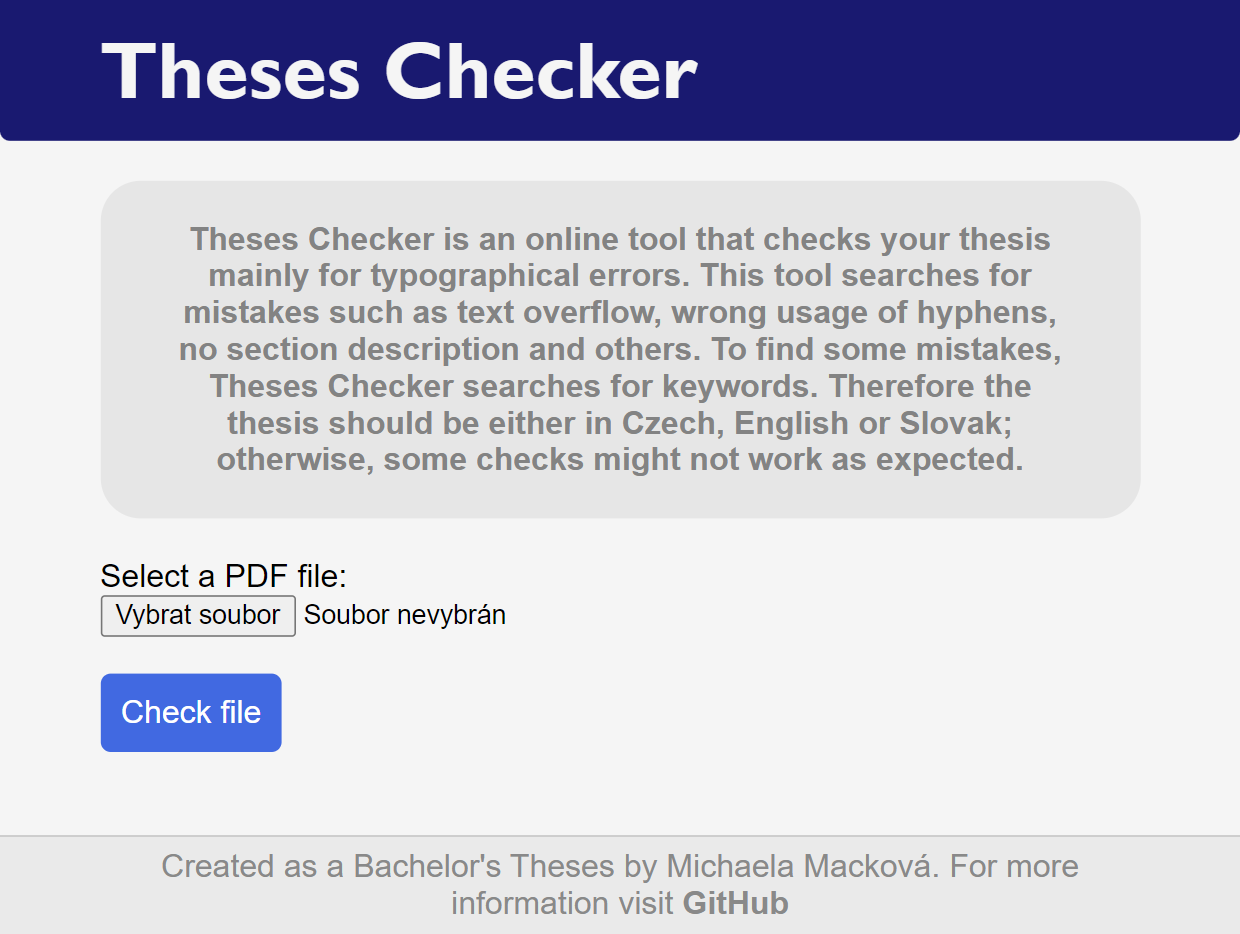
\includegraphics[width=\linewidth]{obrazky-figures/screenshot-page1-small.png}
        \caption{Na tomto obrázku je stránka, která se zobrazí po otevření webové aplikace Theses Checker}
        \label{pic_theses_checker_page1_sub1}
    \end{subfigure}
    \hfill
    \begin{subfigure}[b]{0.496\linewidth}
        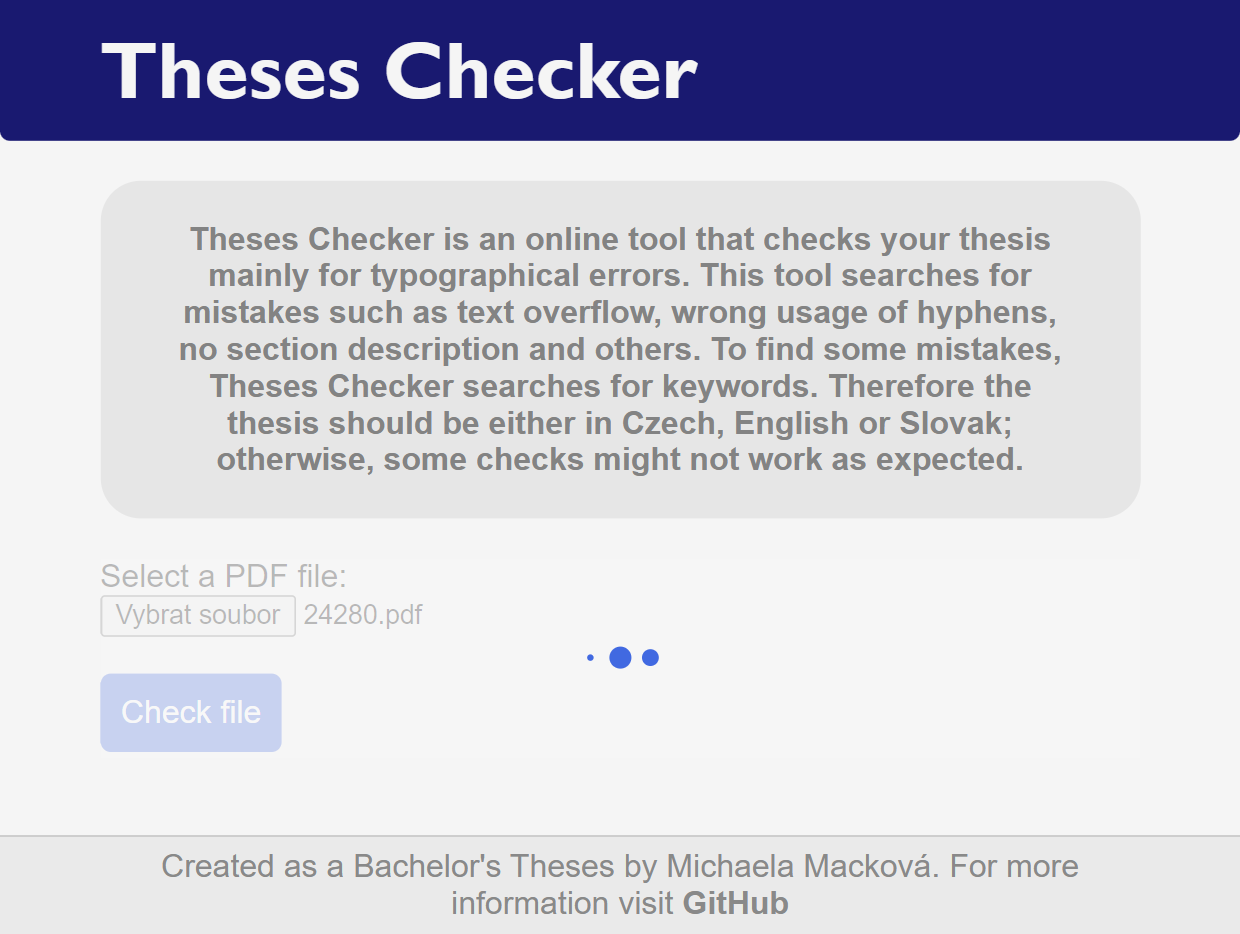
\includegraphics[width=\linewidth]{obrazky-figures/screenshot-loading-small.png}
        \caption{Toto je úvodní stránka s~načítacím elementem, který se zobrazí po stisknutí tlačítka Check file}
        \label{pic_theses_checker_page1_sub2}
    \end{subfigure}
    %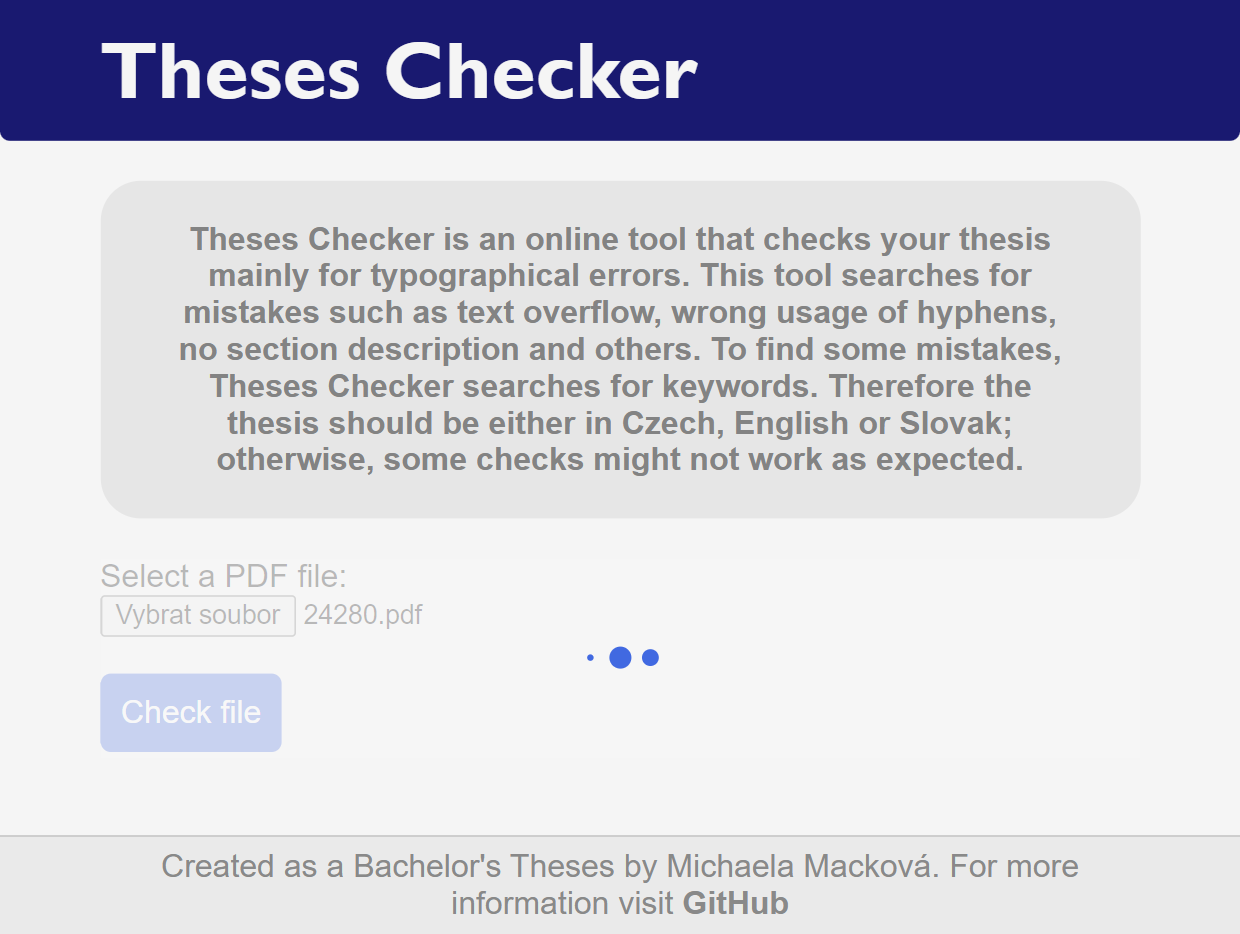
\includegraphics[width=0.496\linewidth]{obrazky-figures/screenshot-loading-small.png}
    \caption[]{Obrázky ukazují úvodní stránku vytvořené webové aplikace Theses Checker}
    \label{pic_theses_checker_page1}
\end{figure}

\begin{figure}[H]
    \centering
    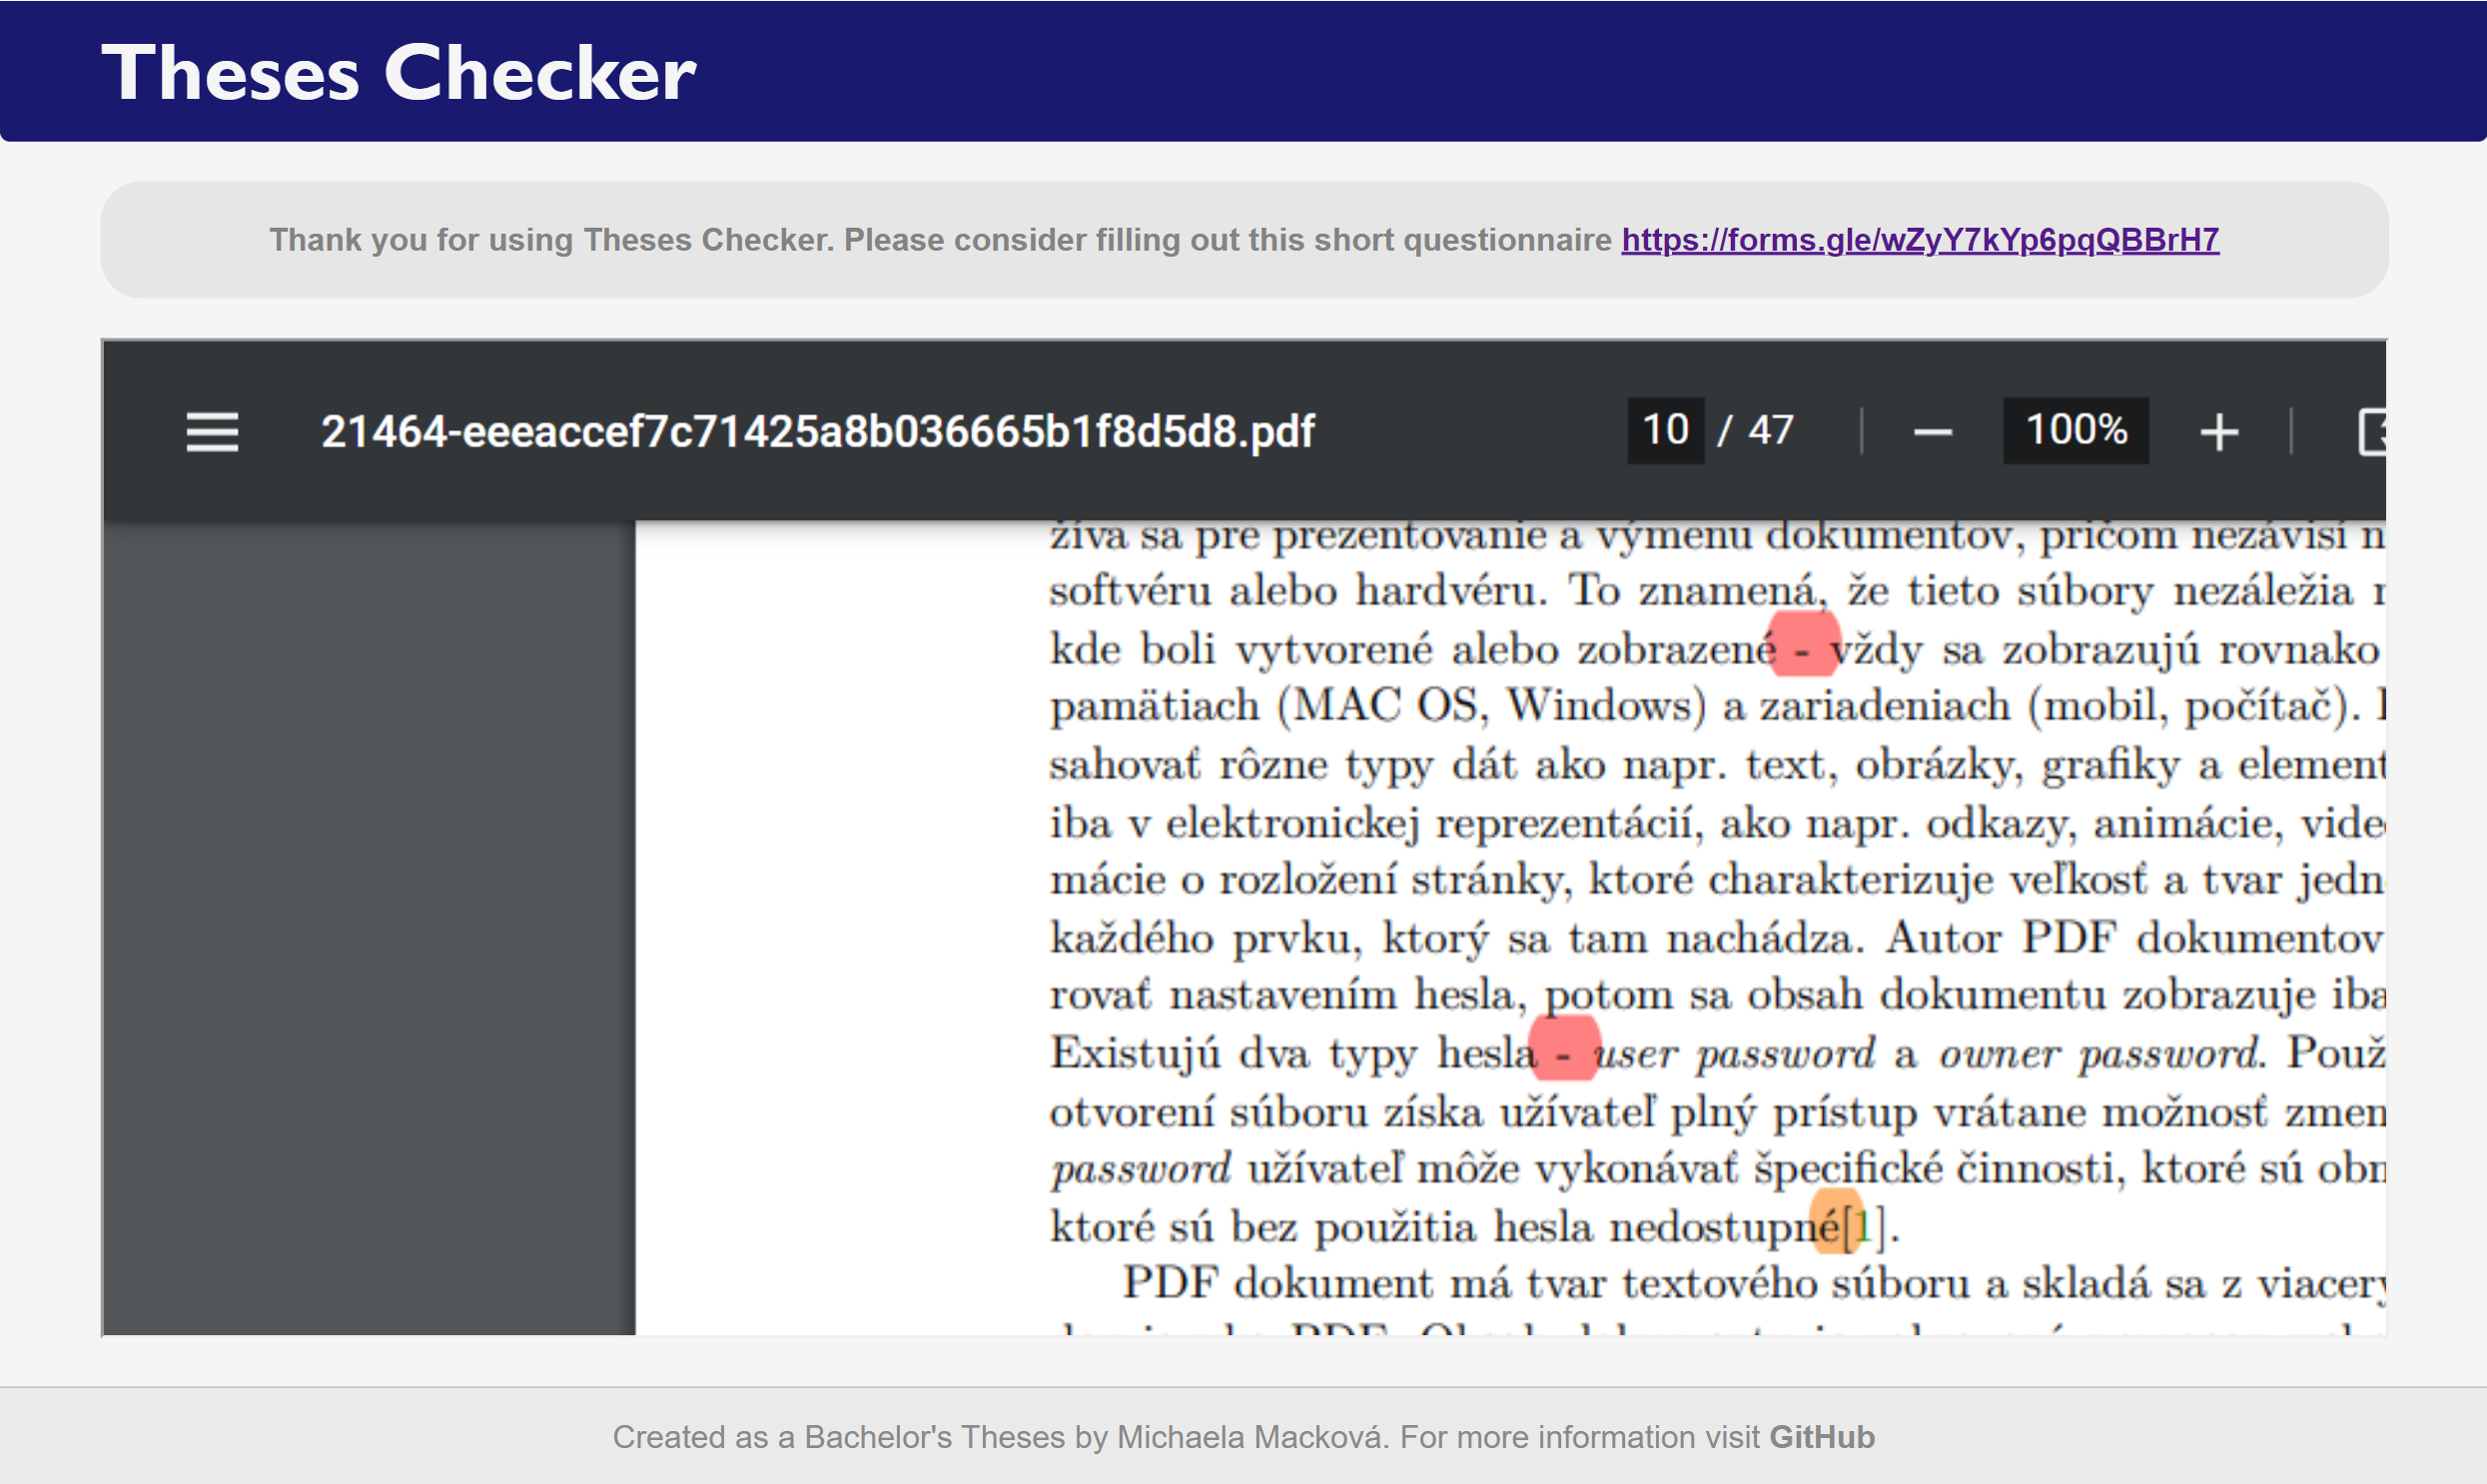
\includegraphics[width=\linewidth]{obrazky-figures/screenshot-page2.png}
    \caption{Tento obrázek ukazuje webovou stránku s~výstupem z~vytvořené aplikace}
    \label{pic_theses_checker_page2}
\end{figure}

V~kapitole~\ref{frequent_mistakes} této bakalářské práce jsou popsány často 
vyskytované chyby
v~diplomových pracích, které byly zjištěny jako součást této práce. Dále je
popsán formát souboru PDF (kapitola~\ref{PDF_file}) a~návrh a~implementace samotné
aplikace (kapitola~\ref{design_implementation}), což zahrnuje i~vývoj webové
aplikace s~pomocí frameworku Django. Kapitola~\ref{testing} poté popisuje postup
testování a~vyhodnocení výsledného produktu.


%*********************************************************************************




%*********************************************************************************
%                                2 ČASTÉ CHYBY
%*********************************************************************************
\chapter{Typografie a~často vyskytované chyby v~diplomových pracích} \label{frequent_mistakes}
U~psaní textu se autor musí řídit nejen gramatickými, ale i~typografickými
pravidly. Toto platí především při psaní odborné práce. Větší množství chyb
v~textu práce může mít za následek to, že i~kvalitně odvedená praktická realizace
práce se bude zdát neuspokojivá.

Chyby mohou být způsobeny z~nepozornosti, anebo z~neznalosti, přičemž druhá možnost
je pro autora textu horší, jelikož i~po několikátém přečtení nemusí pisatel vůbec
poznat, že se jedná o~chybu. Správnou volbou textového editoru si tvůrce textu
může usnadnit hledání některých chyb. Několik dnešních textových procesorů poskytuje
alespoň částečnou kontrolu pravopisu, nicméně tato kontrola umí ve spoustě případů
upozornit převážně jen na překlepy. Významové chyby, jako je například záměna slov
\emph{tip, typ} nebo \emph{autorizace, autentizace}, bývají často touto
automatickou kontrolou zanedbávány. První část této kapitoly popisuje,
čím se zabývá obor typografie a~v~dalších částech je popsáno několik
chyb, které lze nalézt v~mnoha diplomových pracích. Tyto části dále uvádějí,
jak se těmto chybám vyhnout.


%#######################    2.1 Rychlokurz typografie    #######################
\section{Rychlokurz typografie}
Typografie je obor zabývající se návrhem a~úpravou všech druhů tiskovin.
Především se zabývá grafickými prvky (např. obrázky a~písmo) a~jak na člověka
působí celkový vzhled celého díla.
Informace získané z~knihy Praktická typografie~\cite{Prakticka_typografie}
uvádí, že typografie už se rozvíjí přes více jak pět set
let a~základy její práce se téměř neměnily. I~když dříve byla typografická
pravidla důležitá převážně pro sazeče, nyní může pomocí počítače sázet
úplně každý. Toto však zavedlo problém, protože velké množství těchto
uživatelů o~pojmu typografie nikdy neslyšelo. Typografická pravidla se řídí podle
norem, avšak jejich používání není vynutitelné. I~přesto se doporučuje
dodržování těchto typografických pravidel, jelikož při jejich použití
dokáže čtenář lépe vnímat celé dílo. Každý národ má vlastní
soubor typografických pravidel a~při tvorbě cizojazyčného textu by se
měla tato pravidla respektovat.

V~minulosti, kdy se opisovaly knihy ručně, bylo základním prvkem písmeno. 
Základní prvek se od té doby postupně měnil a~nyní je tímto prvkem odstavec.
Nejviditelnější parametr odstavce je zarovnání, které má ve většině 
počítačových sázecích programů čtyři druhy~--~do bloku, doleva, doprava 
a~na střed. Zarovnání odstavce do bloku je běžný v~knižní sazbě a~u~novin
a~časopisů. Dalším důležitým prvkem je písmo, jehož volba je při psaní textu
důležitá. Častý problém je, že některá písma neobsahují kompletní znakovou
sadu, tedy s~tímto písmem nelze vysázet speciální české (či jiné) znaky.
Pro sazbu češtiny nebo slovenštiny je potřeba použít písmo, které obsahuje
minimálně všechny znaky použitého jazyka.

Po umístění textu na stránce se typografie ještě zabývá umístěním samotných
znaků, jako je například otazník, pomlčka či uvozovka. Pro matematickou sazbu, 
chemickou sazbu a~sazbu not je nejlepší použít specializovaný program, 
který obsahuje potřebné funkce. Jeden z~takových programů je právě \TeX,
nebo je též možné použít vzorce z~MS Wordu.



%#######################    2.2 Přetečení objektů za okraj stránky    #######################
\section{Přetečení objektů za okraj stránky}
Přetečení textu za okraj se nejčastěji vyskytuje, když student píše svou diplomovou
práci s~pomocí jazyka {\LaTeX}. Obvykle je to způsobeno tím, že program nedokáže
automaticky zalomit slovo na konci řádku, jak je ukázáno na
obrázku~\ref{pic_overflow}. Toto lze opravit napověděním možného
zalomení problematického slova nebo přeformulováním věty, kde se daná chyba vyskytuje.
Další typ této chyby je přetečení obrázku za okraj,
který se nestává tak často, ale lze jej udělat v~několika textových editorech.

\begin{figure}[H]
    \centering
    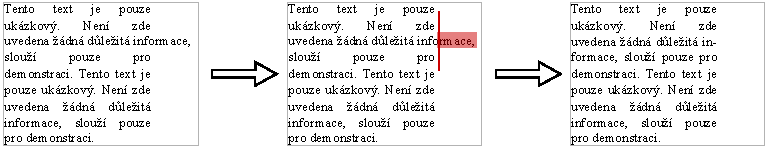
\includegraphics[width=\linewidth]{obrazky-figures/overflow_example.pdf}
    \caption{
        Tento obrázek obsahuje ukázku textu, který přetéká za hranici stránky,
        označení tohoto přetečení a~jeho následnou opravu
    }
    \label{pic_overflow}
\end{figure}


%#######################    2.3 Spojovník x pomlčka    #######################
\section{Chybné použití spojovníku}
Nesprávné používání spojovníku je chyba, která se vyskytuje nejen v~diplomových
pracích. Spojovník (-) je graficky velmi podobný pomlčce (--), ale významově
se značně liší. Pravidla pro psaní těchto znaků, uvedena v~internetové příručce
Ústavu pro jazyk český~\cite[Sekce: \emph{Spojovník} a~\emph{Pomlčka}]{Ustav_pro_jazyk_cesky},
říkají, že spojovník se píše bez mezer mezi výrazy, které spojuje. Výjimkou
je, naznačuje-li spojovník neúplné slovo. Obecně se tedy v~češtině tento znak
užívá, chce-li autor vyjádřit, že jím spojené výrazy tvoří těsný významový
celek. Pomlčka se oproti spojovníku využívá pro oddělování částí projevu,
vyjádření rozsahu, vztahu nebo vyznačení přestávky v~řeči, pro uvození
přímé řeči a~pro vyjádření celého čísla při psaní peněžních částek.
Odděluje se z~obou stran mezerami. Komplikovanější situace nastane pouze
tehdy, když je toto znaménko použito ve funkci výrazů a, až, od, do nebo proti.
Spojovník (-) i~pomlčka (--) bývají často zaměňovány se znaménkem minus ($-$),
to však má též své grafické i~významové odlišnosti.
V~knize Průvodce tvorbou dokumentů~\cite[k.~19.24, s.~148--149]{Pruvodce_tvorbou_dokumentu}
je vysvětleno, že znak minus má stejnou
šíři i~umístění jako znak plus. Znak minus se používá ve dvou významech, a~to
pro označení záporné hodnoty, nebo pro označení operace odčítání. Sazba se v~obou
případech liší: pro označení záporné hodnoty se znak minus a~následující
operand píše bez mezery, pro psaní minus jako odčítání se však mezera uvádí
z~obou stran tohoto znaménka. Internetová příručka Ústavu pro jazyk
český~\cite[Sekce: \emph{Pomlčka}]{Ustav_pro_jazyk_cesky} 
však uvádí, že je v~korespondenci dovoleno
znak minus ($-$) nahradit pomlčkou (--).

Podle článku Základy typografie~\cite{Zaklady_typografie:Slezakova} se tato chyba (naznačena na
obrázku~\ref{pic_hyphen}) vyskytuje v~textu kvůli absenci znaku pomlčky na klávesnici.
Místo znaku pomlčky, který se při psaní textu pravděpodobně používá častěji,
se na klávesnici vyskytuje právě znak spojovníku. I~když nyní už spousta
textových editorů dokáže automaticky nahradit spojovník za pomlčku, tato náhrada
nemusí být stoprocentní. V~programu {\LaTeX} se spojovník zapíše přímo
z~klávesnice jako \verb|-|,
pomlčku je možno zapsat pomocí dvou spojovníků \verb|--| a~znaménko minus je
zapsáno jako spojovník v~matematickém prostředí \verb|$-$| nebo též \verb|$$-$$|.

\begin{figure}[H]
    \centering
    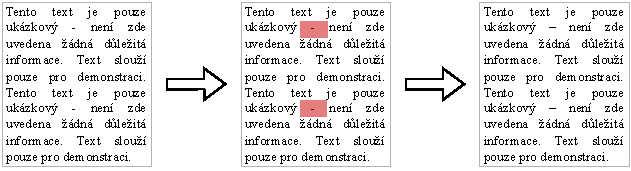
\includegraphics[width=\linewidth]{obrazky-figures/dash_example.pdf}
    \caption{
        Na obrázku je ukázáno chybné použití spojovníku, poté je tato chyba
        označena a~nakonec je ukázáno její opravení
    }
    \label{pic_hyphen}
\end{figure}


%#######################    2.4 Chybějící popis kapitoly    #######################
\section{Chybějící popis kapitoly}

I~když je kapitola rozdělena na několik podkapitol, musí i~samotná kapitola
obsahovat úvod do této kapitoly. Leaný blog~\cite{Leany_blog} vysvětluje, že 
pokud není uveden
popis mezi kapitolou a~její podkapitolou, působí poté práce nedopracovaně. Tuto
skutečnost lze vidět i~na ukázce v~obrázku~\ref{pic_chapter_introduction}. V~tomto místě
se hodí napsat 1--2 odstavce, kde bude vysvětlené, o~čem daná kapitola pojednává a~co se
v~ní čtenář dozví.

\begin{figure}[H]
    \centering
    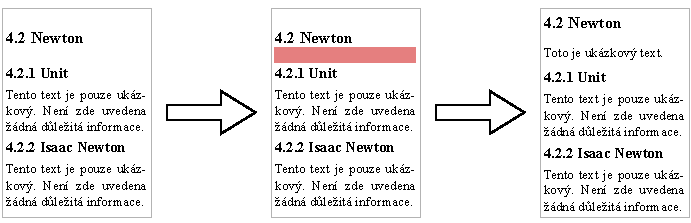
\includegraphics[width=\linewidth]{obrazky-figures/chapter_introduction_example.pdf}
    \caption{
        Obrázek obsahuje ukázku chybějícího popisu kapitoly (tzn. mezi dvěma
        nadpisy se nevyskytuje text). V~další části tohoto obrázku je tato 
        chyba označena a~poté opravena
    }
    \label{pic_chapter_introduction}
\end{figure}


%#######################    2.5 Nadpisy třetí a větší úrovně v obsahu    #######################
\section{Nadpisy třetí a~větší úrovně v~obsahu}
V~diplomové práci není vhodné v~obsahu uvádět nadpisy třetí či větší úrovně.
Jak je vidět na obrázku~\ref{pic_heading}, obsah je poté nepřehledný a~zbytečně
dlouhý. Samotná třetí úroveň nadpisů je velmi podrobná, ale v~diplomové práci
ji lze použít v~případě, když bude nečíslovaná. V~programu {\LaTeX} tohoto lze dosáhnout
příkazem \verb|\subsection*{}|. Nadpisy čtvrté a~větší úrovně by se v~diplomové
práci vyskytovat neměly.

\begin{figure}[H]
    \centering
    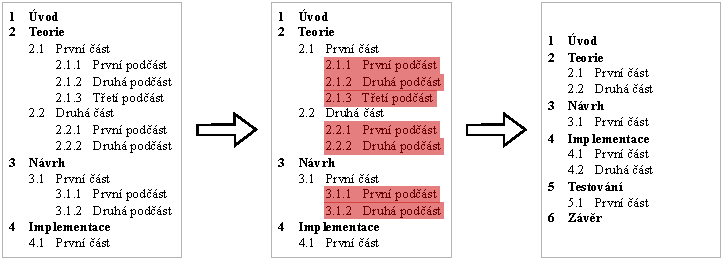
\includegraphics[width=\linewidth]{obrazky-figures/heading_example.pdf}
    \caption{
        Tento obrázek obsahuje ukázku nevhodného uvedení nadpisů třetí
        úrovně v~obsahu, označení nadpisů, které do obsahu nepatří
        a~následnou opravu této chyby
    }
    \label{pic_heading}
\end{figure}


%#######################    2.6 Absence vektorové grafiky    #######################
\section{Absence vektorové grafiky} \label{vector_graphic}
Při vkládání obrázku do textu se autor musí zabývat několika otázkami a~jednou
z~nich je určitě jeho kvalita. Pokud má obrázek moc malé rozlišení,
nevypadá v~odborné práci dobře. I~přesto, že se obrázek na displeji zdá
dostatečně kvalitní, při tisku může být daný obrázek \uv{rozkostičkovaný}.
Toto nevhodné použití lze vidět i~na obrázku~\ref{pic_vector_graphics}.
Tento problém nekvalitního rozlišení může být vyřešen použitím vektorového obrázku.
Podle knihy Průvodce tvorbou dokumentů~\cite[k.~10, s.~56--61]{Pruvodce_tvorbou_dokumentu} 
je zásadní výhodou vektorového
obrázku jeho uložení, díky kterému si obrázek ponechá vysokou kvalitu i~v~různém
zvětšení. Ale použití vektorové grafiky není vždy vhodné a~v~některých případech
není ani možné. V~knize je proto uvedeno doporučení použít vektorovou grafiku
(formáty SVG, EPS a~PDF) na schémata a~loga, rastrovou grafiku formátu JPG pro
fotografie a~pro ostatní rastrovou grafiku použít formát PNG.

\begin{figure}[H]
    \centering
    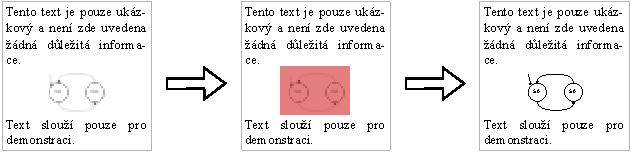
\includegraphics[width=\linewidth]{obrazky-figures/vector_graphics_example.pdf}
    \caption{
        Na tomto obrázku je uvedena ukázka absence vektorové grafiky, dále je
        tato chyba označena a~nakonec je ukázáno její opravení použitím 
        vektorového obrázku
    }
    \label{pic_vector_graphics}
\end{figure}


%#######################    2.7 Nepoužívání pevné mezery    #######################
\section{Nepoužívání pevné mezery}
Jako spousta jiných věcí, i~psaní mezer má svá pravidla. Jak zmiňuje
článek Jak se vyhnout typografickým hříchům~\cite{Ctenar_12_2015}, i~v~něčem
tak samozřejmém, jako je psaní pouhé
mezery, se často chybuje: mezera se musí psát za tečkou (nebo též čárkou), ne před
ní a~píše se vždy jen jedna, data se píšou ve formátu \emph{d.~m. yyyy}
a~čísla se oddělují mezerou po tisících (s~výjimkou letopočtu). Při psaní se může
stát, že mezera spojující znaky nebo čísla vyjde na konec řádku a~tyto znaky
by se rozdělily. Tento případ lze pozorovat i~na obrázku~\ref{pic_hard_space}.
Pro zamezení takových případů existuje právě pevná (nebo též nedělitelná)
mezera.

Pevná mezera se zobrazí stejně jako normální mezera, ale na rozdíl od normální
mezery, spojí dohromady příslušné znaky a~zablokuje jejich rozdělení na konci
řádku. Podle pravidel internetové jazykové příručky~\cite[Sekce: \emph{Zalomení řádků a~nevhodné výrazy na jejich konci}]{Ustav_pro_jazyk_cesky}
se má pevná mezera použít v~těchto případech (převzato a~upraveno):
\begin{itemize}
    \item ve spojení neslabičných předložek \emph{k, s, v, z} s~následujícím
    slovem, např. \emph{v~obrázku, z~funkce},
    \item ve spojení slabičných předložek \emph{o, u} a~spojek \emph{a, i}
    s~následujícím výrazem, např. \emph{o~kapitole, a~to},
    \item členění čísel, např. $\mathit{2\,301\,000}$, $\mathit{3,\!141\,592\,65}$,
    \item mezi číslem a~značkou, např. \emph{25~\%, \copyright~2008},
    \item mezi číslem a~zkratkou počítaného předmětu nebo písmennou značkou
    jednotek a~měn, např. \emph{24~hod., 100\,m, 3\,000~Kč, 500~¥},
    \item mezi číslem a~názvem počítaného jevu, např. \emph{obrázek~5, 12~metrů,
    I.~patro},
    \item v~kalendářních datech mezi dnem a~měsícem, rok však lze oddělit, např.
    \emph{3.~5. 2000, 26.~dubna 2023}
    \item v~měřítkách map, plánů a~výkresů, v~poměrech nebo při naznačení dělení,
    např. \emph{4~:~7, 1~:~10~000}, $\mathit{12:2=6}$,
    \item v~telefonních, faxových a~jiných číslech členěných mezerou, např. 
    \emph{+420~603~999~226},
    \item ve složených zkratkách (v~případě nutnosti se doporučuje dělit podle
    dílčích celků), v~ustálených spojeních a~v~různých kódech, např.
    \emph{s.~r.~o., m~n.~m., ISO~690},
    \item mezi zkratkami typu \emph{tj., tzv., tzn.} a~výrazem, který za nimi
    bezprostředně následuje, např. \emph{tzv.~pipeline},
    \item mezi zkratkami rodných jmen a~příjmeními, např. \emph{T.\,Milet},
    \item mezi zkratkou titulu nebo hodnosti uváděnou před osobním jménem, např.
    \emph{p.~Macková, Ing.~Novák}.
\end{itemize}

Zapsání pevné mezery závisí na použitém textovém editoru. I~když spousta z~nich
již umí tuto pevnou mezeru automaticky doplnit, nemusí mít tato automatizace
stoprocentní úspěšnost. V~programu {\LaTeX} se pevná mezera zapíše znakem tildy
(\texttildelow) a~v~editoru WORD se zapíše pomocí kombinace kláves
\emph{Ctrl Shift mezera}.

\begin{figure}[H]
    \centering
    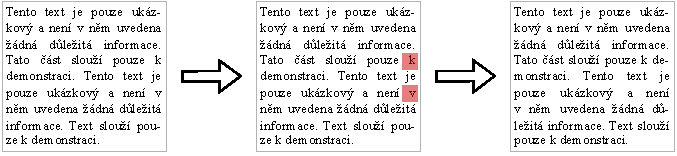
\includegraphics[width=\linewidth]{obrazky-figures/hard_space_example.pdf}
    \caption{
        Tento obrázek obsahuje ukázku zalomení řádku na místě, kde by se měla
        vyskytovat pevná mezera. V~druhé části je tato chyba označena a~v~poslední
        části je uvedeno její možné opravení použitím nezlomitelné mezery
    }
    \label{pic_hard_space}
\end{figure}

%#######################    2.8 Použití nesprávných uvozovek    #######################
% \section{Použití nesprávných uvozovek}
% \dummyText
% \todoimage{width=\linewidth,height=1.7in}{Ukázka.}

% %#######################    2.9 Špatný odkaz na referenci    #######################
% \section{Špatný odkaz na referenci}
% \dummyText
% \todoimage{width=\linewidth,height=1.7in}{Ukázka.}


%*********************************************************************************




%*********************************************************************************
%                               3 ANOTACE V PDF
%*********************************************************************************
\chapter{PDF soubor} \label{PDF_file}
Tato kapitola popisuje strukturu PDF dokumentu. Přesněji popisuje vnitřní
strukturu a~uložení objektů. Dále popisuje, jak funguje grafické zobrazení
PDF dokumentů. V~neposlední řadě je představeno několik knihoven, které
dokáží s~PDF dokumenty manipulovat.



%#######################    3.1 Formát PDF    #######################
\section{Formát PDF} \label{format_PDF}
Většina uživatelů, kteří zachází s~PDF soubory, nepotřebují znát vnitřní složení
PDF dokumentů. Spousta programů a~knihoven pro vytváření či úpravu PDF dokumentu
dokáže při práci s~tímto souborem dostatečně odstínit od syntaxe PDF formátu.
Avšak pro pokročilejší práci s~PDF dokumenty není na obtíž si zjistit pár
základních informací o~uložení dat v~tomto formátu.
PDF dokument má podobu textového souboru a~pro jeho pochopení jsou v~této sekci
vysvětleny jeho 4~základní stavební bloky. Tato sekce čerpá informace ze
standardu PDF~32000-1~\cite[k.~7, s.~11--109]{PDF32000-1:2008}.


%---------- 3.1.1 Objekty ----------
\subsection*{Objekty}
Objekty jsou jedny ze základních stavebních bloků PDF dokumentu. PDF rozeznává
osm typů objektů:
\begin{itemize}
    \item \textbf{Boolean objekt} -- Tyto objekty reprezentují logickou hodnotu.
    Můžou nabýt dvou hodnot, které jsou označeny klíčovými slovy \texttt{true}
    a~\texttt{false}.
    
    \item \textbf{Číselný objekt} -- Obsahovaná číselná hodnota může být celé,
    nebo reálné číslo. U~zápisu reálných čísel se používá desetinná tečka,
    například \texttt{-3.62}, \texttt{.054}, \texttt{+238.45}. Celá čísla můžou
    být například \texttt{500}, \texttt{+3}, \texttt{-21}.
    
    \item \textbf{Řetězcový objekt (string)} -- Řetězec lze zapsat dvěma způsoby,
    a~to jako klasický řetězec, nebo jako řetězec v~hexadecimální podobě. Klasický
    řetězec je zapsán jako posloupnost znaků uzavřená v~kulatých závorkách,
    například \texttt{(Toto je string)}. V~tomto typu řetězce je možné používat
    escape sekvence začínající zpětným lomítkem. Řetězec psaný v~hexadecimální
    podobě lze zapsat jako posloupnost hexadecimálních číslic uzavřenou mezi znaky
    menší než a~větší než, například \texttt{<48656c6c6f>}, \texttt{<776F726C64>}.
    Každá dvojice hexadecimálních číslic tvoří jeden znak zakódovaný v~ASCII
    podobě.
    
    \item \textbf{Jmenný objekt} -- Objekt jména je sekvence znaků. Znaky, které
    se mohou použít ve jménu jsou takové, které zapadají do rozmezí mezi znakem
    vykřičníku (!) a~znakem tildy (\texttildelow). Ostatní znaky se mohou zapsat
    jako hexadecimální hodnota požadovaného znaku, kterou předchází znak mřížky
    (\#). Jméno musí začínat lomítkem, které se nebere jako jeho součást. Zapsané
    jméno může být například \texttt{/Name}, \texttt{/1.6*xyz}, \texttt{/C\#23}.
    
    \item \textbf{Objekt pole} -- Objekt typu pole je kolekce, která obsahuje
    objekty. Tyto objekty nemusí být stejného typu -- heterogenní pole.
    Zapisuje se jako prvky pole, které jsou odděleny bílým znakem, uzavřené
    v~hranatých závorkách. Prvkem pole může být objekt pole. Validní pole je
    například \texttt{[(string) -25 [2.75 /Name] true]}.
    
    \item \textbf{Slovníkový objekt} -- Slovník je kolekce, jejíž prvky jsou
    dvojice objektů. První prvek z~této dvojice se nazývá \emph{klíč} a~vždy to 
    musí být objekt typu jméno. Ve slovníku nesmí existovat více záznamů se
    stejným klíčem. Druhý prvek ze dvojice se nazývá \emph{hodnota}.
    Tento prvek může být objekt jakéhokoli typu. Slovník je uvozen dvojitým znakem
    menší než a~dvojitým znakem větší než, například
    \texttt{<</Key1 2.6 /Key2 /Value2>>}.

    \item \textbf{Objekt datového toku (stream)} -- Stream je sekvence bajtů, 
    která má neomezenou délku. Používá se především pro ukládání velkého množství
    dat, což je například obrázek. Tento objekt se zapisuje jako slovník, za nímž
    následuje klíčové slovo \texttt{stream}, po kterém se musí vyskytovat konec
    řádku. Následují bajty datového toku, které jsou ukončeny koncem řádku
    a~klíčovým slovem \texttt{endstream}. Slovník nesmí být uveden
    nepřímým odkazem a~musí se v~něm uvádět délka datového toku v~bajtech (pod
    klíčem \texttt{Length}). Každý objekt datového toku musí být zároveň nepřímým
    objektem (vysvětleno později v~této sekci). Validní objekt datového toku je
    například uveden ve výpise~\ref{code_stream}:
    \pdfcode{code_examples/pdf_code/stream_objects.txt}{
        V~tomto výpisu je uveden příklad nepřímého objektu
        s~identifikátorem~\texttt{12~0}. Tento nepřímý objekt je zároveň objekt
        datového toku s~velikostí 20\,B, který musí být pro přečtení dekódován 
        FlateDecode filtrem
    }{code_stream}

    \item \textbf{Null objekt} -- Null objekt je speciální objekt, který nabývá
    pouze hodnoty \texttt{null}.
\end{itemize}

Každému objektu se může přiřadit jednoznačný identifikátor, takový objekt se poté
nazývá \textbf{nepřímý objekt}. Na nepřímý objekt potom může být odkazováno
z~jiného objektu, čehož je často využíváno například ve slovníku, kde je uveden
klíč a~hodnota je nepřímý odkaz na objekt. Identifikátor nepřímého objektu má dvě
části. První část je kladné celé číslo, kterému se říká \emph{číslo objektu}.
Druhou částí je tzv. \emph{číslo generace}, které je pro nově generovaný dokument
0. Toto číslo musí být vždy nezáporné celé číslo. Nepřímý objekt se zapíše jako
číslo objektu, poté bílý znak a~číslo generace. Následuje samotný objekt uzavřen
mezi klíčovými slovy \texttt{obj} a~\texttt{endobj}. Validní nepřímý objekt je
uveden ve výpise~\ref{code_indirect_object}:
\pdfcode{code_examples/pdf_code/indirect_object.txt}{
    Tento výpis obsahuje příklad nepřímého řetězcového objektu
    s~identifikátorem~\texttt{7~0}
}{code_indirect_object}
\noindent Nepřímý objekt lze referencovat pomocí \emph{nepřímého odkazu}.
Nepřímý odkaz se zapíše číslem objektu, číslem generace a~klíčovým slovem
\texttt{R}, oddělené bílými znaky. Odkaz na nepřímý objet, který je uveden ve
výpise~\ref{code_indirect_object}, se zapíše jako \texttt{7 0 R}.


%---------- 3.1.2 Struktura souboru ----------
\subsection*{Struktura souboru}
Tato část popisuje, jak jsou výše popsané objekty uložené v~PDF dokumentu.
Též popisuje, jak je k~nim přistupováno a~jak jsou aktualizovány.
PDF soubor se je rozdělen do 4~částí: 
\begin{itemize}
    \item \textbf{Hlavička} -- Hlavička se vždy vyskytuje na prvním řádku souboru.
    Má tvar komentáře, přesněji \texttt{\%PDF–} a~bezprostředně za tím následuje
    číslo PDF verze, například \texttt{\%PDF–1.7}.
    
    \item \textbf{Tělo} -- Tělo se skládá z~posloupnosti nepřímých objektů. Tyto 
    nepřímé objekty popisují vzhled celého dokumentu (stránky, fonty, obrázky,
    \ldots).
    
    \item \textbf{Tabulka křížových odkazů} -- Tabulka křížových odkazů se používá
    při přístupu k~nepřímým objektům. Tato tabulka obsahuje informaci o~umístění
    každého nepřímého objektu. Tabulka se skládá z~jedné nebo více \emph{sekcí
    křížových odkazů}, která musí začínat řádkem s~klíčovým slovem \texttt{xref}.
    Každá sekce může být rozdělena na několik \emph{podsekcí křížových odkazů}.
    Tyto podsekce vždy začínají řádkem, na kterém se vyskytují dvě čísla. První
    číslo označuje první objekt v~záznamu podsekce a~druhé číslo značí, kolik
    takových záznamů se v~dané podsekci vyskytuje. Pod tímto řádkem se nachází
    samotné záznamy o~nepřímých objektech. Záznam o~využívaném nepřímém objektu
    má tvar \emph{nnnnnnnnnn ggggg \texttt{n}} a~je zakončen koncem řádku.
    Desetimístné číslo \emph{nnnnnnnnnn} označuje offset bajtů od začátku
    dokumentu po začátek nepřímého objektu. Pětimístné číslo \emph{ggggg} je
    číslo generace. Jedna možná sekce křížových odkazů je uvedena ve 
    výpisu~\ref{code_cross_reference_table}:
    \pdfcode{code_examples/pdf_code/cross_reference_table.txt}{
        Výpis obsahuje jednu sekci křížových odkazů. Tato sekce je rozdělena
        na 2~podsekce a~celkem obsahuje 3~záznamy
    }{code_cross_reference_table}
    
    \item \textbf{Patička} -- Patička umožňuje rychlé nalezení tabulky křížových
    odkazů a~jiných speciálních objektů. Proto obecně platí, že by se měl PDF
    soubor číst od konce, kde se vykytuje právě patička. Patička začíná klíčovým
    slovem \texttt{trailer}, za ním následuje slovník patičky a~klíčové slovo
    \texttt{startxref}. Na novém řádku se poté vykytuje číslo, uvádějící počet
    bajtů offsetu od začátku souboru po začátek tabulky křížových odkazů. Jako
    poslední se na samostatném řádku musí objevit výraz \texttt{\%\%EOF}.
    V~celém souboru se může vyskytovat více patiček, to je způsobeno aktualizováním
    daného PDF dokumentu. Na posledním řádku souboru se vždy musí vyskytovat
    výraz \texttt{\%\%EOF}. Možná patička je vypsána ve výpisu~\ref{code_trailer}:
    \pdfcode{code_examples/pdf_code/trailer.txt}{
        V~tomto výpisu je uvedena možná patička PDF souboru. Z~této patičky lze
        vyčíst, že tabulka křížových odkazů má celkem 12 záznamů a~její poslední
        sekce začíná na 565.~bajtu. Dále lze zjistit, že nepřímý objekt 
        s~identifikátorem~\texttt{3 0} je
        dokumentový katalog a~metadata dokumentu jsou obsaženy 
        ve slovníkovém nepřímém objektu s~identifikátorem~\texttt{1 0}
    }{code_trailer}

\end{itemize}

Tyto 4~části jsou v~PDF souboru seřazeny v~takovém pořadí, v~jakém jsou zde
sepsané. Tyto části jsou vyznačeny v~ukázkovém souboru, který je ukázán
na obrázku~\ref{pic_file_structure}.

\begin{figure}[H]
    \centering
    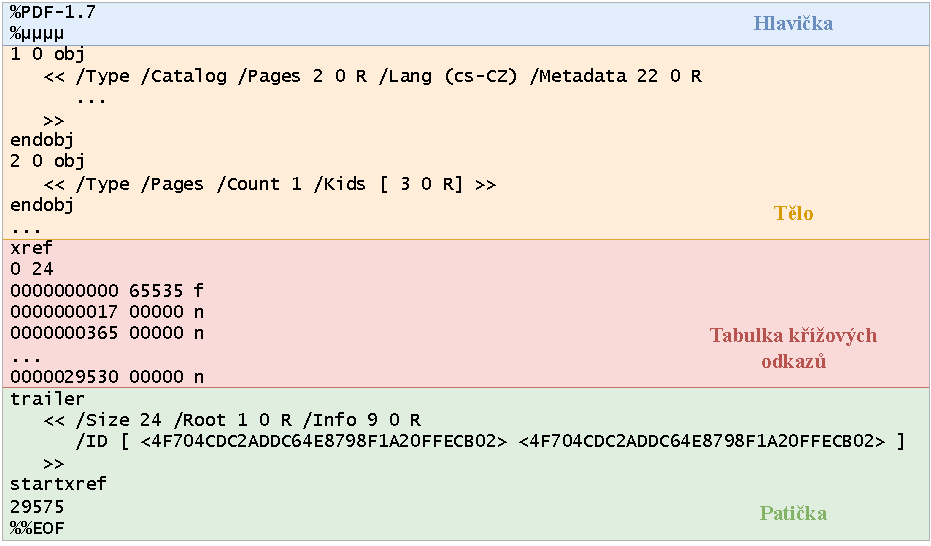
\includegraphics[width=\linewidth]{obrazky-figures/file_structure.pdf}
    \caption{
        Na obrázku se vyskytuje ukázkový PDF soubor, ve kterém jsou vyznačeny 
        4~části struktury PDF souborů 
    }
    \label{pic_file_structure}
\end{figure}


%---------- 3.1.3 Struktura dokumentu ----------
\subsection*{Struktura dokumentu} \label{document_structure}
Struktura dokumentu popisuje, jak vypadá vyobrazený PDF dokument. Na rozdíl
od struktury souboru, která popisuje vnitřní rozložení, si ji
lze představit jako hierarchii objektů vyskytujících se v~těle PDF souboru.
Některé z~důležitých částí tohoto hierarchického stromu jsou:
\begin{itemize}
    \item \textbf{Katalog dokumentu} -- Tento katalog je kořenem celého
    hierarchického stromu. Odkaz na něj lze nalézt ve slovníku patičky pod klíčem
    \texttt{Root}. Tento katalog obsahuje odkazy na objekty specifikující vzhled
    dokumentu. Objekt katalogu je slovník, ve kterém se musí vyskytovat klíč
    \texttt{Type}, ke kterému je přiřazena hodnota \texttt{/Catalog}. Dalším
    povinným prvkem katalogového slovníku je klíč \texttt{Pages}, jehož hodnota je
    nepřímý odkaz na kořenový objekt stromu stránek. Příklad objektu katalogu
    dokumentu je uveden ve výpisu~\ref{code_document_catalog}:
    \pdfcode{code_examples/pdf_code/document_catalog.txt}{
        Tento výpis obsahuje příklad katalogu dokumentu, ze kterého lze zjistit,
        že kořen stromu stránek je nepřímý objekt s~identifikátorem~\texttt{5 0}
    }{code_document_catalog}

    \item \textbf{Strom stránek} -- Strom stránek určuje pořadí zobrazení stránek.
    Listové uzly tohoto stromu jsou typu \emph{objektu stránky}, které mají jiný
    tvar než ostatní uzly tohoto stromu. Uzly stromu stránek jsou typu slovník,
    ve kterém se musí vyskytovat klíče \texttt{Type}, \texttt{Kids},
    \texttt{Count} a~\texttt{Parent}, jenž není povinný v~kořenovém uzlu.
    Hodnota klíče \texttt{Type} musí v~uzlu stromu stránek být \texttt{/Pages}.
    Ke klíči \texttt{Kids} musí být přiřazena hodnota typu pole, které obsahuje
    nepřímé odkazy na uzly stromu stránek, nebo na objekty stránek. Hodnota klíče
    \texttt{Count} je počet listových uzlů, které jsou potomkem tohoto uzlu. Ke
    klíči \texttt{Parent} je přiřazena hodnota nepřímého odkazu přímého předchůdce
    tohoto uzlu. Platný uzel stromu je uveden ve výpisu~\ref{code_page_tree}:
    \pdfcode{code_examples/pdf_code/page_tree.txt}{
        Výpis obsahuje jeden uzel stromu stránek. Potomci tohoto uzlu jsou
        nepřímé objekty s~identifikátorem~\texttt{21~0} a~\texttt{24~0}
        a~celkově existuje 10 listových uzlů (objektů stránek), které
        jsou potomky tohoto uzlu
    }{code_page_tree}

    \item \textbf{Objekt stránky} -- Objekt stránky je typ listového uzlu stromu
    stránek. Tento uzel má tvar slovníku, ve kterém se musí vyskytovat klíč
    \texttt{Type} s~hodnotou \texttt{/Page}. Dalším povinným záznamem tohoto
    slovníku je klíč \texttt{Parent}, jehož hodnota je nepřímý odkaz na přímého
    předchůdce tohoto listového uzlu stromu stránek. Mezi jiné důležité záznamy
    patří záznamy s~klíčem \texttt{MediaBox}, \texttt{Resources}, \texttt{Rotate},
    \texttt{Contents}, \texttt{Annots} aj.
    Možný objekt stránky je obsažen ve výpisu~\ref{code_page_object}:
    \pdfcode{code_examples/pdf_code/page_object.txt}{
        Tento výpis obsahuje jednoduchý objekt stránky, jejíž content stream
        je obsažen v~nepřímém objektu s~identifikátorem~\texttt{10~0} a~resources
        použity v~tomto content streamu jsou vypsané v~nepřímém objektu
        s~identifikátorem~\texttt{9~0}
    }{code_page_object}
\end{itemize}


%---------- 3.1.4 Content streams ----------
\subsection*{Content streams} \label{content_streams}
Content stream obsahuje popis vzhledu PDF stránky pomocí instrukcí na její
vykreslení. Tyto instrukce jsou zapsány pomocí PDF objektů, ale na rozdíl od
PDF dokumentu, jsou tyto instrukce seřazené a~vykonávají se podle jejich
posloupnosti. \emph{Operand} takové instrukce musí být přímý objekt, který 
nesmí být typu datového toku. Operand může být typ slovník pouze při použití
speciálních operací. \emph{Operátor} instrukce určuje, která akce se provede.
Operátory jsou klíčová slova typu jmenného objektu, kde se na rozdíl od jmenných objektů v~těle 
PDF dokumentu operátory píšou bez počátečního lomítka. Content stream používá pro zapsání
instrukcí postfixovou notaci, tedy nejdříve jsou uvedeny všechny operandy instrukce
a~poté je uveden její operátor.


%---------- 3.1.5 Resources ----------
\subsection*{Resources} \label{resources}
Resources specifikují a~pojmenovávají používané externí objekty z~content streams.
V~content streams se nesmí používat nepřímé odkazy, proto je možné pojmenovat
jednotlivé používané objekty a~definovat je tak jako \emph{named resources}.
Tyto jména lze používat pouze uvnitř content streams a~mimo ně nejsou v~těle PDF
dokumentu validní. Named resources se používají například pro obrázky a~fonty,
které jsou použity na dané stránce. Objekt pro resources je typu slovník, který
má několik definovaných klíčů, které je možné použít, např. \texttt{ColorSpace}, 
\texttt{XObject}, \texttt{Font}, \texttt{ProcSet} a~další. Příklad slovníku pro
resources je uveden ve výpisu~\ref{code_resources}:
\pdfcode{code_examples/pdf_code/resources.txt}{
    V~tomto výpisu je uveden slovník pro resources, který obsahuje jeden font pod 
    jménem \texttt{F5} a~dva externí objekty pojmenované jako \texttt{Im1} 
    a~\texttt{Im2}
}{code_resources}



%#######################    3.2 Grafika v~PDF    #######################
\section{Grafika v~PDF}
Tato sekce čerpá informace ze standardu PDF~32000-1~\cite[k.~8, s.~110--236]{PDF32000-1:2008}.
Grafika PDF dokumentu je popsána pomocí content streams, jenž je vysvětleno
v~kapitole~\ref{content_streams}. Operátory zde používané spadají do šesti
hlavních skupin:
\begin{itemize}
    \item \textbf{Graphics state operátory} -- Tyto operátory manipulují
    s~datovou strukturou zvanou \emph{graphics state}, která je vysvětlena později
    v~této kapitole.
    \item \textbf{Operátory pro konstrukci křivek} -- Jsou to operátory, které
    specifikují, jak bude vypadat vykreslená křivka. Spadají sem například
    operátory pro vytvoření nové cesty, přidávání zaoblení, přidávání nové části
    křivky a~uzavření tvaru.
    \item \textbf{Operátory pro vymalování křivek} -- Jsou to operátory vybarvující
    křivku nebo prostor vyhrazený takovou křivkou.
    \item \textbf{Další vykreslovací operátory} -- Tyto operátory se používají
    pro vykreslení grafických objektů, mezi které patří i~obrázky.
    \item \textbf{Textové operátory} -- Text se v~PDF dokumentu vykreslí jako několik
    grafických částí, které jsou definovány fontem. Pomocí těchto operátorů
    se specifikují nastavení spojené s~textem a~též sem patří operátory pro
    vykreslení takového textu. 
    \item \textbf{Marked-content operátory} -- Tyto operátory přímo neovlivňují
    vzhled stránky, ale spojují informace a~objekty uvedené v~content streamu.
\end{itemize}


%---------- 3.2.1 Souřadnicové systémy ----------
\subsection*{Souřadnicové systémy}
PDF definuje více souřadnicových systémů, ve kterých se definují různé grafické
objekty. Převod mezi těmito souřadnicovými systémy se provádí s~pomocí
transformačních matic, které dokážou otáčet, posunovat nebo měnit měřítko
mapovaného objektu (nemění se přitom samotné data uloženého objektu, jen jak je
zobrazen uvnitř souřadnicového systému). V~PDF se transformační matice značí polem
obsahujícím šest číselných objektů $[a~b~c~d~e~f]$. Tato transformační matice je
vyobrazena v~rovnici~\eqref{transformation_matrix}.
\begin{equation}\label{transformation_matrix}
    M_T = 
    \begin{pmatrix}
        a & b & 0 \\
        c & d & 0 \\
        e & f & 1
    \end{pmatrix}
\end{equation}
Pokud je potřeba provést více elementárních transformací 
(např. rotace a~posun), záleží na jejich posloupnosti provedení. Obecně
platí vzorec~\eqref{multiple_matrix_transformations}, kde $M_{T_1}$ značí matici
první provedené transformace, $M_{T_n}$ je matice poslední provedené transformace
a~$M'$ označuje matici, která kombinuje všechny tyto provedené transformace.
\begin{equation} \label{multiple_matrix_transformations}
    M' = M_{T_1} \cdot M_{T_2} \cdots M_{T_{n-1}} \cdot M_{T_n}
\end{equation}

Bod $(x, y)$ v~souřadnicovém systému se může matematicky popsat jako vektor
z~rovnice~\eqref{point}.
\begin{equation}\label{point}
    \overrightarrow{p}  = 
    \begin{pmatrix}
        x & y & 1
    \end{pmatrix}
\end{equation}
Transformovaný bod (souřadnice bodu po použití všech transformací) se vypočítá
pomocí vzorce~\eqref{transform_point}. $\overrightarrow{p}$ v~tomto vzorci označuje původní vektor
transformovaného bodu, $\overrightarrow{p'}$ je vektor tohoto bodu po transformaci a~$M'$ je matice
kombinující všechny provedené transformace.
\begin{equation} \label{transform_point}
    \overrightarrow{p'} = \overrightarrow{p} \cdot M'
\end{equation}

Dále jsou popsány souřadnicové systémy používané v~PDF. Vztahy mezi těmito
souřadnicovými systémy jsou vyznačeny na obrázku~\ref{coordinate_spaces}.
\begin{itemize}
    \item \textbf{Prostor zařízení (device space)} -- Tento souřadnicový systém je
    závislý na zařízení, kde se zobrazuje vytvořený PDF dokument. Je to poslední
    prostor, do kterého se promítá zobrazení PDF souboru. Zobrazovacím zařízením
    se rozumí například displej obrazovky počítače, papír v~tiskárně, plátno, na
    které promítá projektor aj.
    
    \item \textbf{Uživatelský prostor (user space)} -- Aby se zamezilo nevhodným
    účinkům při zobrazování do prostoru zařízení, definuje PDF vlastní prostor,
    který je nezávislý na zařízení. Tento souřadnicový systém se nazývá
    \emph{uživatelský prostor}. Pro každou stránku PDF dokumentu se tento
    souřadnicový systém uvede do původního stavu. V~uživatelském prostoru je bod
    $(0, 0)$ levý dolní roh, tedy x-ová souřadnice se zvyšuje směrem
    doprava a~y-ová souřadnice roste směrem nahoru. Rozlišení určeno v~jednotkách
    uživatelského prostoru nesouvisí s~rozlišením v~pixelech uvnitř prostoru
    zařízení. Převedení z~uživatelského prostoru do prostoru zařízení se provádí
    pomocí \emph{current transformation matrix (CTM)}. CTM je součástí datové
    struktury \emph{graphics state}, která je popsána dále v~této kapitole.
    Aplikace zobrazující PDF si tuto CTM matici upraví podle vlastností výstupního
    zařízení, aby se zachovala nezávislost uživatelského prostoru na zařízení. 
    Vyobrazení tohoto jevu jde vidět na obrázku~\ref{pic_user_to_device}.

    \begin{figure}[H]
        \centering
        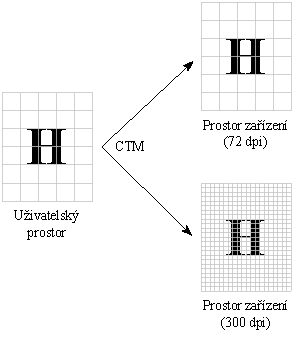
\includegraphics[width=0.5\linewidth]{obrazky-figures/user_to_device_space.pdf}
        \caption{
            V~tomto obrázku je ukázána transformace z~uživatelského prostoru
            do dvou různých prostorů zařízení, kde jeden má rozlišení 72\,DPI 
            a~druhý má 300\,DPI. CTM představuje current transformation matrix
            získanou z~datové struktury graphics state.
            Obrázek je převzatý a~upravený ze
            standardu~PDF~32000-1~\cite[k.~8.3.2.3, s.~116]{PDF32000-1:2008}
        }
        \label{pic_user_to_device}
    \end{figure}
    
    \item \textbf{Specializované prostory} -- PDF formát pracuje kromě
    uživatelského prostoru a~prostoru zařízení i~se specializovanými prostory.
    \begin{itemize}
        \item \emph{Textový prostor} -- V~tomto prostoru se definují souřadnice
        textu. Převod z~textového prostoru do uživatelského prostoru se provádí
        pomocí \emph{textové matice} a~několika textových parametrů vyskytujících
        se v~datové struktuře graphics state.

        \item \emph{Glyph space} -- Glyfy\footnote{
            Glyf je grafické znázornění grafému (písmena, číslice, znaku, piktogramu, interpunkčního a~jiných znamének).
        }
        znaků fontu musí být definovány v~tomto
        prostoru. Z~glyph space se poté transformuje do textového prostoru.
        
        \item \emph{Obrázkový prostor} -- Všechny obrázky by měly být definovány
        v~tomto prostoru. Pro správné vykreslení obrázku na stránku se musí dočasně
        upravit CTM.

        \item \emph{Prostor formuláře} -- Formulářový \emph{XObject} (též externí
        objekt, viz dále v~této kapitole) je
        reprezentován jako content stream. Tento XObject je v~jiném content streamu
        brán jako grafický objekt. Prostor, ve kterém je tento formulář definovaný,
        se nazývá prostor formuláře.

        \item \emph{Pattern space} -- PDF formát poznává typ barvy zvaný
        \emph{pattern}. Pattern je definovaný jako content stream a~prostoru, ve
        kterém je definován, se říká pattern space.
        
        \item \emph{3D prostor} -- Tento souřadnicový systém je
        trojdimenzionální a~používá se pro vložené 3D díla.
    \end{itemize}
\end{itemize}

\begin{figure}[H]
    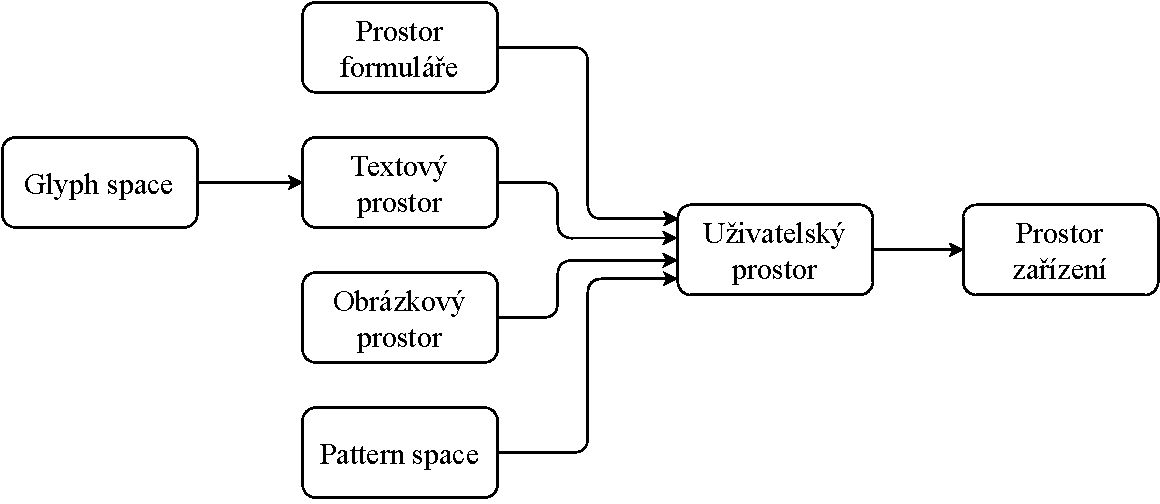
\includegraphics[width=\linewidth]{obrazky-figures/coordinate_spaces.pdf}
    \caption[Vztah mezi souřadnicovými systémy používaných uvnitř PDF]{
        Obrázek označuje vztah mezi souřadnicovými systémy používaných uvnitř
        PDF. Každá šipka představuje transformaci mezi dvěma souřadnicovými 
        systémy. Obrázek je převzatý a~upravený ze 
        standardu~PDF~32000-1~\cite[k.~8.3.3, s.~117]{PDF32000-1:2008}
    }
    \label{coordinate_spaces}
\end{figure}


%---------- 3.2.2 Graphics state ----------
\subsection*{Graphics state} \label{graphics_state}
Pro zobrazení PDF dokumentu se používá datová struktura zvaná \emph{graphics state}.
Každá aplikace zobrazující PDF dokumenty musí umět udržovat tuto datovou strukturu.
Graphics state struktura v~sobě obsahuje několik parametrů, se kterými pracují
operace uvnitř content streamu (popsaný v~kapitole~\ref{content_streams}). Pro
každou stránku se na začátku musí v~graphics state struktuře nastavit výchozí
hodnoty obsahujících parametrů. Tyto parametry jsou rozděleny na dvě skupiny:
závislé na zařízení a~nezávislé na zařízení. Mezi parametry nezávislých na zařízení
patří například CTM (current transformation matrix), barva (aktuální barva
používaná při vykreslovacích operacích), stav textu (devět parametrů popisující
formát vypisovaného textu) a~tloušťka čáry. Parametry závislé na zařízení jsou
například \uv{overprint}, \uv{flatness} a~\uv{smoothness}.

Na jedné stránce se může vyskytovat několik grafických objektů, které se
vykreslují nezávisle na sobě. Pro tyto účely se používá
\emph{graphics state zásobník}, díky kterému je možné dělat lokální úpravy 
datové struktury graphics state. Tento zásobník je LIFO (last in, first out)
a~ukládá se do něj celá datová struktura graphics state, jak je ukázáno na
obrázku~\ref{pic_graphics_state}. Pro uložení
se musí použít operátor \texttt{q} a~pro odebrání první položky z~vrcholu
zásobníku se musí použít operátor \texttt{Q}, kterým se obnoví posledně uložený
stav datové struktury graphics state. Uvnitř celého content streamu musí být
použit stejný počet operátorů \texttt{q} a~\texttt{Q}.

\begin{figure}[H]
    \centering
    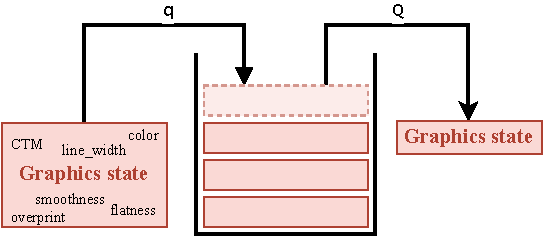
\includegraphics[width=0.7\linewidth]{obrazky-figures/graphics_state_stack.pdf}
    \caption{
        Na tomto obrázku je ukázán graphics state zásobník, do kterého se ukládá
        pomocí příkazu \texttt{q} a~odebírá se z~něj příkazem \texttt{Q}
    }
    \label{pic_graphics_state}
\end{figure}

Pro úpravu parametrů uložených ve struktuře graphics state se používají uvnitř
content streamu specifické operátory. Mezi tyto operátory patří již uvedené
\texttt{q} a~\texttt{Q}, které nepoužívají žádné operandy. Další používané
operátory upravující graphics state jsou například \texttt{cm}, \texttt{w},
\texttt{i} a~jiné. K~operátoru \texttt{cm} se váže šest číselných operandů
\emph{a, b, c, d, e} a~\emph{f}. Dohromady tyto operandy specifikují matici
transformace, která bude vynásobena maticí CTM a~následně přiřazena do CTM položky
datové struktury graphics state. Operátor \texttt{w} je unární a~jeho operandem
je číslo \emph{lineWidth}, které specifikuje tloušťku kreslených čar. Unární
operátor \texttt{i} nastaví uvedený číselný operand jako \emph{flatness} parametr
struktury graphics state.



%---------- 3.2.3 Externí objekty ----------
\subsection*{Externí objekty} \label{XObject}
Externí objekt (též taky \emph{XObject}) je grafický objekt, jehož vzhled
je definován v~samostatném datovém toku.
Každý XObject lze vykreslit pomocí operátoru \texttt{Do} vyskytujícího se uvnitř
content streamu (více informací o~content streamu je uvedeno 
v~sekci~\ref{content_streams}). K~tomuto operátoru se váže jeden operand typu 
jméno. Toto jméno
musí být uvedeno ve slovníku resources (viz kapitola~\ref{resources}) vázaného
na stejnou stránku jako content stream. Přesněji se toto jméno musí objevit
v~položce pod klíčem \texttt{XObject}, která má hodnotu typu slovník. Operátor
\texttt{Do} má 3~různá chování. Toto chování závisí na hodnotě vázané ke klíči
\texttt{Subtype} uvnitř XObject slovníku, na který se odkazuje operand tohoto
příkazu. Hodnoty klíče \texttt{Subtype} a~k~nim vázané chování příkazu
\texttt{Do} jsou:
\begin{itemize}
    \item \texttt{/Image} -- Tyto externí objekty mají ve slovníkové části své
    definice dodatečné prvky. Některé tyto prvky můžou ovlivnit, jak bude
    vykreslený obrázek vypadat, ale podle aktuálního nastavení stránky můžou mít
    omezené možnosti. Prvky s~klíčem \texttt{Width} a~\texttt{Height}
    jsou v~těchto objektech povinné a~vyjadřují výšku a~šířku původního obrázku
    (uvedeného ve streamu tohoto externího objektu). Pro vykreslení
    tohoto objektu na stránce se používá operátor \texttt{Do}, který 
    pomocí parametrů uvnitř datové struktury graphics state (vysvětlena dříve
    v~této sekci) správně upraví a~vykreslí tento objekt.
    
    \item \texttt{/Form} -- Takzvaný \emph{Form XObject} je takový, který ve svém
    datovém toku obsahuje content stream (popsán v~sekci~\ref{content_streams}).
    Form XObject může být vykreslen několikrát, a~to na různých souřadnicích.
    Ve slovníkové části tohoto objektu musí být pro tento typ uvedena hodnota
    pro klíč \texttt{BBox}. Tato hodnota jsou souřadnice daného externího objektu
    v~prostoru formuláře. Pro transformaci mezi formulářovým prostorem a~user
    space se uvádí použitá transformační matice jako hodnota pro klíč
    \texttt{Matrix}. Pokud tato matice není uvedena, použije se místo ní
    jednotková matice. Pro vykreslení se tohoto objektu se musí použít operátor
    \texttt{Do} a~při tom se provedou následující kroky (převzato ze standardu
    PDF~\cite[k.~8.10.1, s.~218]{PDF32000-1:2008}):
    \begin{enumerate}
        \item Uloží se aktuální stav datové struktury graphics state, stejně
        jako kdyby byl použit operátor \texttt{q}.
        \item Vynásobí se matice ze slovníkového prvku \texttt{Matrix} a~matice
        CTM z~datové struktury graphics state.
        \item Ostřihne se na základě slovníkového prvku \texttt{BBox}.
        \item Vykreslí obsahované  grafické objekty podle instrukcí uvnitř content
        streamu definovaného objektem form XObject.
        \item Obnoví původní stav struktury graphics state (jako použití operátoru
        \texttt{Q}).
    \end{enumerate}
    
    \item \texttt{/PS} -- Takzvaný \emph{PostScript XObject} je využíván pouze,
    pokud bude daný PDF dokument zpracován zařízením používající jazyk PostScript.
    Při zobrazení v~jiných zařízeních bude tento objekt ignorován. Aplikace
    zpracovávající PDF dokumenty nemají nutnost zpracování těchto objektů
    podporovat.
\end{itemize}


%#######################    3.3 Reprezentace anotací v PDF souboru    #######################
\section{Reprezentace anotací v~PDF souboru} \label{PDF_annotations}
Anotace spojují objekty (zvuk, video, text, \dots) s~pozicí na PDF stránce.
Uživatel může s~anotacemi interagovat pomocí myši a~klávesnice.
Pokud se na stránce vyskytují nějaké anotace, všechny tyto anotace jsou vypsány
v~objektu dané stránky (více viz sekce~\ref{document_structure}). Přesněji
se v~tomto objektu vyskytuje prvek s~klíčem \texttt{Annots}, který má jako 
hodnotu pole, které obsahuje nepřímé odkazy na objekty anotací vyskytovaných
na dané stránce.
PDF dokumenty podporují několik typů anotací, 
například:
\begin{itemize}
    \item \textbf{Text} -- Tyto anotace imitují nalepovací papírky. Jsou
    zobrazeny jako ikona umístěna na určitých souřadnicích a~po interakci s~myší
    se zobrazí vyskakovací okénko s~textem této anotace. Tato anotace ignoruje
    rotaci a~změnu měřítka stránky. Ve slovníku této anotace se můžou navíc
    objevit záznamy s~klíčem \texttt{Subtype} (tento prvek je povinný a~pro tento
    typ anotace musí mít hodnotu \texttt{/Text}), \texttt{Open}, \texttt{Name},
    \texttt{State} a~\texttt{StateModel}. Příklad textové anotace lze vidět ve
    výpisu~\ref{code_text_annotation}:
    \pdfcode{code_examples/pdf_code/text_annotation.txt}{
        Anotace typu \emph{Text}, která se zobrazí jako ikona
        \emph{Note}. Po interakci s~myší se zobrazí vyskakovací okénko
        s~textem \uv{This is text annotation.}
    }{code_text_annotation}

    \item \textbf{Odkaz} -- Anotace odkazu slouží jako hypertextový
    odkaz na místo v~daném dokumentu, nebo jako akce, která se má
    provést po jejím stisknutí. Ve slovníku takové anotace musí
    existovat povinný záznam s~klíčem \texttt{Subtype}, který musí mít hodnotu
    \texttt{/Link}. Další možné záznamy mohou být \texttt{A},
    \texttt{Dest}, \texttt{H}, \texttt{PA}, \texttt{QuadPoints}
    a~\texttt{BS}. Validní anotace odkazu je uvedena ve
    výpisu~\ref{code_link_annotation}:
    \pdfcode{code_examples/pdf_code/link_annotation.txt}{
        Anotace typu \emph{Link}, která odkazuje na místo uvnitř
        stejného dokumentu.
    }{code_link_annotation}
    
    \item \textbf{Volný text} -- Tato anotace bude na stránce
    zobrazena jako viditelný text. Ve slovníku její definice
    musí být uveden záznam \texttt{Subtype} s~hodnotou
    \texttt{/FreeText} a~záznam \texttt{DA}, kterým se definuje
    grafická úprava vypsaného textu. Slovník může obsahovat další
    záznamy, například \texttt{Q}, \texttt{IT} nebo \texttt{BS}.
    
    \item \textbf{Přímka} -- Tato anotace se na stránce zobrazí
    jako jedna definovaná přímka. Po její interakci s~myší se
    může zobrazit vyskakovací okénko. \texttt{Subtype} záznam ve slovníku, který
    definuje tuto anotaci, musí mít hodnotu \texttt{/Line}. Další
    povinný záznam je \texttt{L}, jehož hodnota specifikuje počáteční 
    a~konečný bod dané přímky. V~tomto slovníku je možné uvést
    ještě několik dalších záznamů, například \texttt{BS}, \texttt{IC},
    \texttt{Cap} a~\texttt{LE}.
    
    \item \textbf{Označení textu} -- Označení textu anotacemi se může zobrazit
    jako jeho zvýraznění, podtržení, vlnité podtržení, nebo jeho přeškrtnutí.
    Pro zvolení typu označení se musí ve slovníku této anotace uvést příslušná
    hodnota povinného záznamu \texttt{Subtype}, a~to \texttt{/Highlight},
    \texttt{/Underline}, \texttt{/Squiggly}, nebo \texttt{/StrikeOut}.
    Další povinný záznam této anotace je \texttt{QuadPoints}, jehož hodnota
    specifikuje souřadnice čtyřúhelníku, ve kterém je obsažen označovaný text.
    Této anotaci může být přiřazena vyskakovací anotace.
    
    \item \textbf{Vyskakovací anotace} -- Toto vyskakovací okénko je vždy spojené
    s~jinou anotací (takzvanou \emph{rodičovskou anotací}). Samotná nemá
    definovaný žádný datový tok popisující vhled, ani k~sobě nemá přiřazenou
    žádnou akci. Bývá uvedena jako nepřímý odkaz ve slovníku své rodičovské
    anotace (přesněji v~záznamu \texttt{Popup}).
\end{itemize}



%#######################    3.4 Programovací jazyky a knihovny pro zpracování a anotování PDF souborů    #######################
\section{Programovací jazyky a~knihovny pro zpracování a~anotování PDF souborů}

Pro zpracovávání PDF souborů existuje mnoho knihoven v~různých programovacích
jazycích. Výběr programovacího jazyka záleží nejen na požadavcích pro výslednou
aplikaci, ale též na znalostech daného programátora. Samotná knihovna se poté
vybere na základě její funkcionality. 

V~této kapitole jsou popsány různé knihovny, které je možné použít pro zpracování
PDF souborů, jejich speciality a~nedostatky.


%---------- 3.3.1 C# ----------
\subsection*{C\#}

Dokumentace jazyka C\#~\cite{CSharp} říká, že  C\# je objektově orientovaný 
programovací jazyk, vyvinutý firmou Microsoft.
Jazyk C\# je potomkem rodiny jazyků C. Je jim tedy podobný a~programátorům těchto
jazyků nebude dlouho trvat se jej naučit. Jazyk C\# je jeden z~nejpoužívanějších
jazyků pro vývoj na platformě .NET.

Nejznámější C\# knihovna pro práci s~PDF dokumenty je \textbf{iText 7}
(informace byly získány z~její oficiální dokumentace~\cite{iText_7}). 
Tato knihovna je dostupná pod \emph{Open Source AGPLv3}\footnote{
\href{https://itextpdf.com/how-buy/AGPLv3-license}{https://itextpdf.com/how-buy/AGPLv3-license}
} licencí a~dvěma verzemi komerční licence. Tato knihovna umí vytvářet nové
i~upravovat již existující PDF dokumenty. Pomocí této knihovny lze například
přidávat anotace, hlavičky a~patičky stránek, spojovat několik dokumentů do
jednoho, upravovat metadata, vyplňovat či upravovat formuláře a~extrahovat 
text či~jiné PDF objekty.


%---------- 3.3.2 JavaScript ----------
\subsection*{JavaScript}
Podle webové stránky věnované jazyku JavaScript~\cite{JavaScript} je
JavaScript dynamicky typovaný, objektově orientovaný, interpretovaný
programovací jazyk. Nejčastěji se využívá jako skriptovací jazyk používaný
pro vytváření webových stránek, je však často používaný i~mimo prostředí webového
prohlížeče. Nejznámější z~těchto případů je například Node.js, Apache CouchDB
a~Adobe Acrobat. 

Pro zpracování PDF souborů v~jazyce JavaScript je možné použít některou
z~následujících knihoven:
\begin{itemize}
    \item \textbf{PDF.js}\,--\,Informace o~této knihovně byly získány
    z~oficiální dokumentace PDF.js knihovny~\cite{PDFjs}.
    Tato knihovna byla vyvinuta převážně pro čtení a~vykreslování PDF
    souborů, samotná neumí dané soubory editovat. Jiné knihovny jsou s~touto
    knihovnou často kombinovány pro pokročilejší práci s~PDF soubory. Práce
    s~PDF.js knihovnou závisí na využívání takzvaných Promises, bez kterých nelze
    tuto knihovnu používat, proto je doporučené se s~jejich používáním dobře
    seznámit před jakoukoliv prací s~touto knihovnou. PDF.js je dostupné pod
    licencí \emph{Apache License 2.0}\footnote{
    \href{https://github.com/mozilla/pdf.js/blob/master/LICENSE}{https://github.com/mozilla/pdf.js/blob/master/LICENSE}}.
    
    \item \textbf{pdfAnnotate}\,--\,Informace o~této knihovně byly získány
    z~GitHub stránek pdfAnnotate knihovny~\cite{pdfAnnotate}.
    Knihovna pdfAnnotate je vyvinutá specificky pro anotování PDF souborů dostupná pod
    licencí \emph{MIT License}\footnote{
    \href{https://github.com/highkite/pdfAnnotate/blob/master/LICENSE}{https://github.com/highkite/pdfAnnotate/blob/master/LICENSE}
    }. Funguje pouze v~prostředí webového prohlížeče a~Node.js. Samotná knihovna
    neumí číst a~zobrazovat PDF soubory, proto je doporučováno tuto knihovnu
    kombinovat s~výše zmíněnou knihovnou PDF.js. Přidané anotace se zapisují
    na konec PDF souboru, díky tomu je možné je zobrazit i~mimo vytvořenou
    aplikaci.
    
    \item \textbf{PDF-LIB}\,--\,Informace o~této knihovně byly získány
    z~oficiálních stránek PDF-LIB knihovny~\cite{pdf_lib}.
    Tuto knihovnu je možné používat v~jakémkoliv JavaScriptovém prostředí.
    PDF-LIB dokáže vytvářet nové či modifikovat existující PDF soubory. Mezi
    modifikace patří například vytváření a~vyplňování formulářů, vkládání PDF
    stránek a~čtení a~přepisování metadat souboru. Vytváření anotací je možné, ale
    vyžaduje pokročilejší znalost zápisu formátu PDF. Tato knihovna je dostupná
    pod licencí \emph{MIT License}\footnote{
    \href{https://github.com/Hopding/pdf-lib/blob/master/LICENSE.md}{https://github.com/Hopding/pdf-lib/blob/master/LICENSE.md}
    }.
\end{itemize}


%---------- 3.3.3 PHP ----------
\subsection*{PHP}

Informace uvedené na oficiálních PHP stránkách~\cite{PHP_is, PHP_can_do} uvádí,
že PHP je skriptovací programovací jazyk, který je především vhodný pro vývoj
dynamických webových stránek. Často je PHP kód vnořený přímo do HTML kódu, kterému
tak přidává dynamičnost. PHP podporuje objektově orientované i~procedurální 
programování. I~když je PHP jazyk používán převážně pro vývoj webu, lze jej využít
i~pro vytvoření aplikace běžící v~příkazové řádce a~pro vývoj
desktopových aplikací.

\begin{itemize}
    \item \textbf{TCPDF}\,--\,Informace o~této knihovně byly získány
    z~oficiálních stránek TCPDF kni\-hov\-ny~\cite{TCPDF}.
    Tato knihovna je zaměřena na vytváření PDF dokumentů, mezi jejíž hlavní
    vlastnosti patří podpora fontů, automatické hlavičky a~patičky na stránce,
    dělení slov, zarovnání a~zalamování textu, PDF anotace a~automatické číslování
    stran. TCPDF nepodporuje čtení a~editaci existujících PDF souborů.
    Knihovna TCPDF je dostupná pod \emph{Free Software License}\footnote{
    \href{https://tcpdf.org/docs/license/}{https://tcpdf.org/docs/license/}
    } licencí.

    % \item \textbf{TCPDI}\footnote{
    % \href{https://github.com/pauln/tcpdi}{https://github.com/pauln/tcpdi}
    % }\,--\,\todo{text}
    
    % \dummyShortText[8]

    \item \textbf{FPDI}\,--\,Informace o~této knihovně byly získány
    ze stránek FPDI kni\-hov\-ny~\cite{FPDI}.
    Toto je knihovna pro používání stránek z~existujícího PDF dokumentu jako
    šablonu do nového PDF dokumentu. Při opakovaném použití jedné šablony tato 
    knihovna zajistí, že tato šablona bude v~souboru PDF zahrnuta právě jednou. Díky
    této skutečnosti může být výsledné PDF menší velikosti než PDF vytvořeno jiným
    způsobem. Tato třída je kompatibilní s~výše zmíněnou knihovnou TCPDF. Od verze
    1.6 je knihovna FPDI dostupná pod licencí \emph{MIT license}\footnote{
    \href{https://www.tldrlegal.com/l/mit}{https://www.tldrlegal.com/l/mit}
    }.

\end{itemize}


%---------- 3.3.4 Python ----------
\subsection*{Python} \label{python_libraries}

Oficiální dokumentace jazyka Python~\cite{Python} uvádí, že Python je 
vysokoúrovňový, interpretovaný programovací jazyk. Má dynamickou
kontrolu datových typů a~podporuje objektově orientované programování. Tyto
skutečnosti z~něj dělají ideální jazyk pro skriptování a~rychlé prototypování
různých aplikací na mnoho platformách. Python je programovací jazyk vhodný i~pro
začátečníky.

V~tomto jazyce existuje několik knihoven pro práci s~PDF soubory. Je možné použít
například následující: 
\begin{itemize}
    \item \textbf{PyMuPDF}\,--\,Informace o~této knihovně byly získány
    z~oficiální dokumentace PyMuPDF kni\-hov\-ny~\cite{PyMuPDF}.
    Tato knihovna je Python verze knihovny MuPDF. Je dostupná pod dvěma různými licencemi, a~to pod
    licencí \emph{Open Source\,--\,AGPL}\footnote{
    \href{https://artifex.com/licensing/agpl/}{https://artifex.com/licensing/agpl/}
    } a~komerční\footnote{
    \href{https://artifex.com/licensing/commercial/}{https://artifex.com/licensing/commercial/}
    } licencí. Knihovna se může lišit podle verze s~danou licencí. Tato knihovna
    dokáže například číst a~vyjmout text i~obrázky, číst a~upravovat
    metadata a~vyhledávat text v~existujícím dokumentu.
    Knihovna má podporu pro OCR (Optical Character Recognition), pokud při
    instalaci byl nainstalován též balíček Tesseract. Podporované formáty dokumentu jsou
    PDF, XPS, OpenXPS, CBZ, EPUB a~FB2 (eBooks). PyMuPDF umí zacházet
    i~s~populárními formáty obrázků jako jsou PNG, JPEG, BMP, TIFF a~dalšími.
    Knihovna má pro~PDF dokumenty několik funkcí navíc,
    což zahrnuje například vytváření nového dokumentu, extrahování a~přidávání
    fontů a~obrázků, pracování se soubory chráněnými heslem (např. zašifrování 
    a~dešifrování), zcela podporuje práci s~vloženými soubory, plně podporuje 
    práci s~anotacemi a~dokáže vytvářet, číst i~vyplňovat formuláře.

    \item \textbf{pikepdf}\,--\,Informace o~této knihovně byly získány
    z~oficiální pikepdf dokumentace~\cite{pikepdf}.
    Tuto knihovnu lze používat pro vytváření, čtení i~úpravu PDF dokumentů.
    Je to Python verze C++ knihovny QPDF. Pro požívání knihovny je nutné být
    seznámen se specifikací PDF formátu. Knihovna je dostupná pod
    \emph{Mozilla Public License 2.0}\footnote{
    \href{https://github.com/pikepdf/pikepdf/blob/master/LICENSE.txt}{https://github.com/pikepdf/pikepdf/blob/master/LICENSE.txt}
    } licencí. Pikepdf dokáže kopírovat stránky do jiného PDF souboru, extrahovat
    obrázky, nahradit obrázek za jiný, upravovat metadata souboru a~další.

\end{itemize}


%*********************************************************************************




%*********************************************************************************
%                            4 NÁVRH A IMPLEMENTACE 
%*********************************************************************************
\chapter{Návrh a~implementace aplikace Theses Checker} \label{design_implementation}
Součástí této práce byly vytvořeny 2~aplikace, jedena je webový nástroj a~druhá je
program pro použití z~příkazového řádku. Tato kapitola pojednává o~požadavcích na 
vytvářené aplikace a~dále popisuje detaily všech vytvořených programů.


%#######################    4.1 Specifikace požadavků    #######################
\section{Specifikace požadavků}
Cílem vytvořené aplikace je nalézt a~vyznačit chyby, které se vyskytují
v~nahrané technické zprávě. Technická zpráva bude ve formátu PDF.
Požadavky na vytvořený program jsou:
\begin{itemize}
    \item Program musí podporovat technické zprávy napsané v~jazyce českém
    a~s~menší podporou i~v~jazyce slovenském nebo anglickém.

    \item Aplikace musí primárně umět kontrolovat diplomové práce vytvořené
    v~šabloně pro jazyk {\LaTeX}, která byla
    poskytnuta univerzitou Vysoké učení technické v~Brně, přesněji Fakultou
    informačních technologií.

    \item Program musí být lehce přístupný, nejlépe bez nutnosti
    jakékoliv instalace.
    
    \item Aplikace by měla být funkční na co nejvíce platformách, aby byla
    zajištěna dostupnost pro co nejvíce uživatelů.

    \item Aplikace by měla umět pracovat s~co nejaktuálnější verzí PDF.
    
    \item Není nutné, aby program dokázal zpracovat několik PDF dokumentů
    zároveň. Postačí, aby v~jednom příkazu zpracoval právě jeden dokument.
\end{itemize}

Nalezené chyby budou označeny graficky pomocí PDF anotací, jako například
zvýraznění textu a~kreslení čar. Toto označení by mělo být zřetelné -- dobře
viditelné a~na první pohled pochopitelné. Aplikace by tím měla imitovat
poznámky korektora. Detekované chyby jsou takové, které se často vyskytují 
v~technických pracích.
Tyto časté chyby byly zjištěny zkoumáním rozpracovaných i~odevzdaných
diplomových prací a~projevilo se, že vyskytované časté chyby jsou porušení
některého z~typografických pravidel. Tyto nalezené časté chyby jsou uvedeny
v~kapitole~\ref{frequent_mistakes}. 
Aktuálně neexistuje žádná aplikace, která by aktivně kontrolovala typografické
chyby. Většina existujících aplikací hledá pouze porušení gramatických pravidel.
Hledání chyb bude pracovat na principu zvaném \emph{false-positive}. To znamená,
že něco může být označeno jako chyba, ale ve skutečnosti se o~chybu nejedná.



%#######################    4.2 Návrh aplikace    #######################
\section{Návrh aplikace}
Aby byla aplikace co nejvíce nezávislá, byla vyvinuta jako webová aplikace.
Tato aplikace musí být intuitivní a~až na nahrání PDF dokumentu by se nemělo
muset vyplňovat zbytečně mnoho informací. Většina informací by měla být
zjištěna automaticky z~poskytnutého PDF souboru. Jak je ukázáno na
obrázku~\ref{pic_theses_checker_dia}, vstupem této aplikace by měl být
samotný, neupravený PDF dokument, který vytvořená aplikace zpracuje
a~jejím výstupem je tento PDF dokument doplněný o~anotace.

\begin{figure}[H]
    \centering
    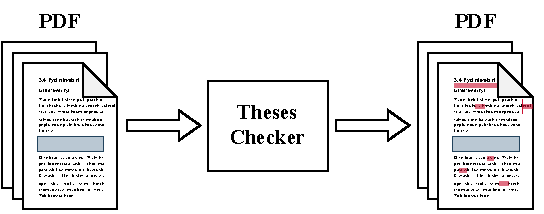
\includegraphics[width=\linewidth]{obrazky-figures/Theses_Checker_diagram.pdf}
    \caption{
        Na tomto obrázku jsou ukázány vstupy a~výstupy aplikace Theses Checker
    }
    \label{pic_theses_checker_dia}
\end{figure}

Vytvořená webová aplikace by měla odrážet tento uvedený vzor vstupů a~výstupů.
Úvodní stránka, jejíž náčrt lze vidět na
obrázku~\ref{pic_theses_checker_design_page1}, slouží pouze pro nahrání
PDF dokumentu, aby se mohl dále zpracovat. Po stisku tlačítka CHECK bude
PDF dokument zpracován, zkontrolován a~anotován. Poté bude uživatel přesměrován na
stránku, jejíž náčrt je ukázán na obrázku~\ref{pic_theses_checker_design_page2}.
Na této stránce bude pro lepší uživatelskou přívětivost přímo zobrazen
anotovaný dokument (místo často používaného odkazu na stáhnutí souboru).

\begin{figure}[H]
    \centering
    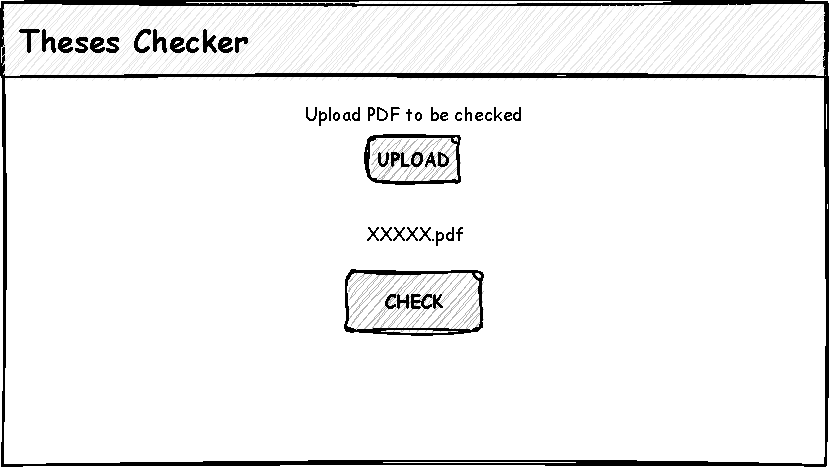
\includegraphics[width=0.8\linewidth]{obrazky-figures/Theses_Checker_design-page1.pdf}
    \caption{
        Tento obrázek obsahuje návrh úvodní stránky webové aplikace Theses Checker
    }
    \label{pic_theses_checker_design_page1}
\end{figure}

\begin{figure}[H]
    \centering
    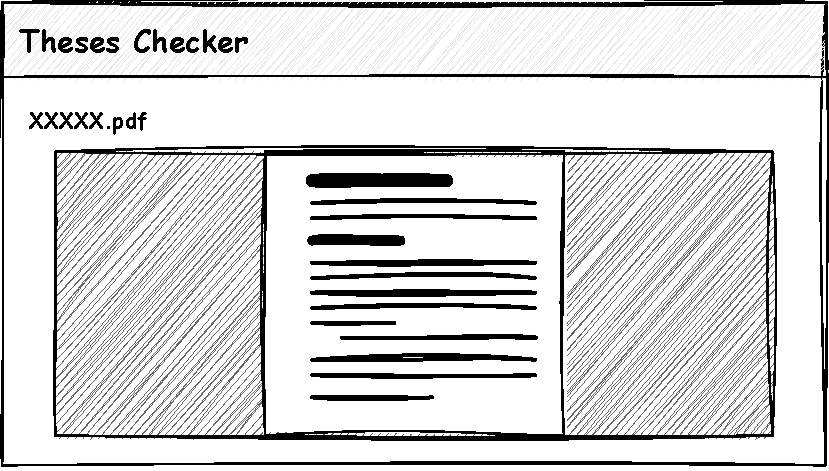
\includegraphics[width=0.8\linewidth]{obrazky-figures/Theses_Checker_design-page2.pdf}
    \caption{
        Tento obrázek obsahuje návrh stránky webové aplikace Theses Checker, kde
        je zobrazeno výstupní PDF
    }
    \label{pic_theses_checker_design_page2}
\end{figure}

Jelikož webová aplikace umí kontrolovat pouze jeden dokument, byla navrhnuta
též konzolová aplikace. Tato konzolová aplikace musí pracovat na podobném
principu, jako je uveden na obrázku~\ref{pic_theses_checker_dia}. Proto
webová i~konzolová aplikace musí používat stejný program, který bude kontrolovat
a~anotovat vstupní PDF dokument.  

Výstupní dokument bude obsahovat několik anotací pro označení nalezených chyb.
Toto označení by mělo být viditelné a~mělo by jasně označovat, co za chybu bylo
nalezeno. Z~tohoto důvodu bylo navrženo používání highlight anotace kombinovanou
s~pop-up anotací. Highlight anotace označí, kde na stránce byla nalezena chyba
a~podrobný popis nalezené chyby je možné zobrazit rozkliknutím pop-up anotace,
která se váže na danou highlight anotaci.



%#######################    4.3 Využité technologie    #######################
\section{Využité technologie}
Pro zpracování všech programových částí této bakalářské práce, byly
využity následující technologie:

\begin{description}
    \item[Python:] Jazyk Python byl zvolen díky knihovně PyMuPDF
    (popsána v~sekci~\ref{python_libraries}), která splňuje nejvíce požadavků
    pro tuto práci. Některé z~požadavků jsou například úprava existujícího PDF
    souboru, přidání základních anotací, extrakce textu a~možnost exportovat
    libovolnou stránku PDF souboru na obrázek (v~tomto případě pixelovou mapu).
    Další funkcí, která byla velmi nápomocná, je zjištění pozice některých
    objektů, které se vyskytují na stránce.

    \item[PythonAnywhere:] PythonAnywhere je služba poskytující hosting webových
    aplikací vytvořených v~jazyce Python. Je to jedna z~mála služeb poskytujících
    verzi 3.10 jazyka Python i~pro své neplatící uživatele. PythonAnywhere
    nabízí pět typů účtu a~mezi nimi je i~účet, který je zcela zdarma. Tento
    účet má několik omezení (např. omezení velikosti datového úložiště na
    512\,MB, neexistující možnost používání vlastní domény a~nutnost alespoň jednoho
    přihlášení a~potvrzení činnosti v~intervalu 3~měsíců), ale pro
    implementovanou aplikaci je dostačující.

    \item[Django:] Django je jeden z~nejznámějších frameworků pro tvorbu webových
    aplikací v~jazyce Python. Tato volba byla závislá právě na vybraném
    programovacím jazyce a~též na službě PythonAnywhere, která má několik
    návodů na nasazení webových aplikací využívajících právě framework Django.
    Django dokumentace je velmi rozsáhlá a~obsahuje i~návod pro vytvoření
    první webové aplikace.
    
    \item[HTML, CSS:] HTML a~CSS jazyky byly použity pro grafickou tvorbu
    zobrazených webových stránek. Upravený jazyk HTML se používá pro tvorbu
    šablon využívaných v~Django frameworku. A~CSS jazyk byl použit pro
    definici grafického stylu zobrazených stránek.
    
    \item[JavaScript:] Jazyk JavaScript byl ve vyvinuté aplikaci použit pro
    částečnou kontrolu, zda je nahraný soubor ve formátu PDF. Další využití
    bylo pro zobrazení načítacího elementu (\uv{poskakujících} teček),
    který je viditelný při čekání na zpracování nahraného PDF dokumentu.
    
\end{description}



%#######################    4.4 Implementace webové aplikace    #######################
\section{Implementace webové aplikace} \label{web_app}
Výsledná webová aplikace byla vyvinuta s~pomocí Django frameworku.
Nahraný soubor se pošle na server pomocí HTTP požadavku metodou POST
a~uloží se ve specifické složce. Poté se pomocí třídy \texttt{Checker}
uložené v~souboru \texttt{theses\_checker.py} (popsáno dále
v~kapitole~\ref{checker}) tento soubor zkontroluje a~přidají se anotace.
Tento výstupní soubor se opět uloží na server do určité složky a~původní soubor
se ze serveru odstraní. Následně bude uživatel přesměrován na stránku, která
zobrazí výstupní anotovaný dokument. Po zobrazení tohoto dokumentu na stránce je
dokument odstraněn ze serveru. Postup zpracování nahraného PDF souboru je
naznačen na obrázku~\ref{pic_communication}.

\begin{figure}[H]
    \centering
    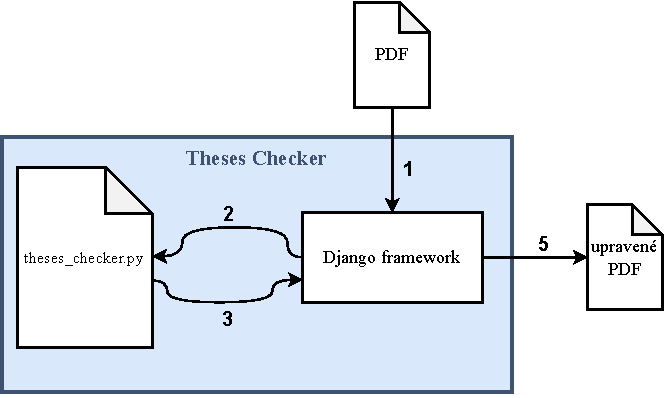
\includegraphics[width=0.8\linewidth]{obrazky-figures/Theses_Checker_communication.pdf}
    \caption{
        Tento obrázek popisuje postup komunikace webové aplikace mezi 
        frameworkem Django a~programem pro vyhledávání chyb v~PDF dokumentu 
    }
    \label{pic_communication}
\end{figure}


%---------- 4.4.1 Architektura webové aplikace ----------
\subsection*{Architektura webové aplikace}
Django pracuje s~architekturou zvanou model-view-template (dále jen MVT),
která je velmi podobná známé architektuře model-view-controller (dále jen MVC).
View má v~architektuře MVT podobnou roli jako controller z~architektury MVC 
a~template z~MVT má podobnou roli jako view z~MVC.

Všechny šablony použité pro webové stránky jsou uloženy ve
složce \texttt{templates} a~každá rozvíjí šablonu zvanou \texttt{base.html}
pro jednotný vzhled. Řídící logika webové aplikace je umístěna v~souboru
\texttt{views.py} a~program pro vyhledání a~označení chyb se vyskytuje 
v~souboru \texttt{theses\_checker.py}. V~souboru \texttt{settings.py}
se před spuštěním musí nastavit tajný klíč (proměnná \texttt{SECRET\_KEY}) 
a~může se zde nastavit, zda server poběží v~módu pro vývoj či nikoliv
(proměnná \texttt{DEBUG}). Server webové aplikace se spustí
pomocí souboru \texttt{manage.py} použitím
příkazu: \verb|$ python manage.py runserver|

Všechny potřebné soubory pro správnou funkci webové aplikace jsou uloženy
ve složce s~názvem \texttt{web}. Hlavní struktura této složky vypadá následovně:

\dirtree{%
.1 \textbf{web}.
.2 \textbf{files}.
.2 \textbf{static}.
.3 \textbf{css}.
.3 \textbf{js}.
.2 \textbf{templates}.
.3 \textbf{theses\_checker}.
.4 annotated.html.
.4 index.html.
.3 400.html.
.3 403.html.
.3 404.html.
.3 500.html.
.3 base.html.
.2 \textbf{theses\_checker}.
.3 \textbf{bl}.
.4 theses\_checker.py.
.3 views.py.
.2 \textbf{web}.
.3 settings.py.
.2 manage.py.
}



%---------- 4.4.2 Implementační detaily ----------
\subsection*{Implementační detaily}
Během vývoje webové aplikace se vyskytlo několik problémů, které se převážně
podařilo vyřešit. Jeden takový problém bylo, v~jaký moment se ze serveru odstraní
výstupní soubor. Jelikož server má omezené úložiště (v~případě neplaceného účtu
služby PythonAnywhere je to 512\;MB), musí se všechny poskytnuté i~vytvořené PDF
dokumenty někdy odstranit. Vstupní dokument se odstraní ihned po vytvoření
výstupního dokumentu. Tento výstupní dokument se nejdříve musí zobrazit na
webové stránce, až poté může být odstraněn. Použité řešení využívá
odpovědi\footnote{
    Odpověď dostupná na:
    \href{https://groups.google.com/g/django-users/c/Da8HvVts9pI/m/fwgaFj8RAAAJ}{https://groups.google.com/g/django-users/c/Da8HvVts9pI/m/fwgaFj8RAAAJ}
} nalezené na google groups, ve které se tento problém řeší uložením
obsahu PDF souboru do proměnné, vymazáním souboru ze serveru a~následným posláním 
obsahu vytvořené proměnné jako HTTP odpovědi. Ve vytvořené webové aplikaci se tato
HTTP odpověď přijímá do HTML elementu \texttt{<iframe>}, který se vyskytuje na
zobrazované webové stránce. Aby mohl element \texttt{<iframe>} zobrazit webovou
stránku, musí se u~této zobrazované stránky nastavit X-Frame-Options. Díky
odpovědi\footnote{
    Odpověď lze nalézt na 
    \href{https://stackoverflow.com/a/33267908}{https://stackoverflow.com/a/33267908}
} ze Stack Overflow bylo možné správně nastavit tuto možnost. 

Dalším detailem bylo zobrazení chybových stránek. Django má podporu pro nastavení
šablony chybových stránek s~chybovým kódem 400, 403, 404 a~500. S~každým tímto
chybovým kódem se pojí jedna šablona, jejíž soubory se jmenují \texttt{400.html},
\texttt{403.html}, \texttt{404.html} a~\texttt{500.html}. Příklad chybové
stránky, která se zobrazí při nahrání poškozeného souboru, lze vidět na
obrázku~\ref{pic_theses_checker_error}.

\begin{figure}[H]
    \centering
    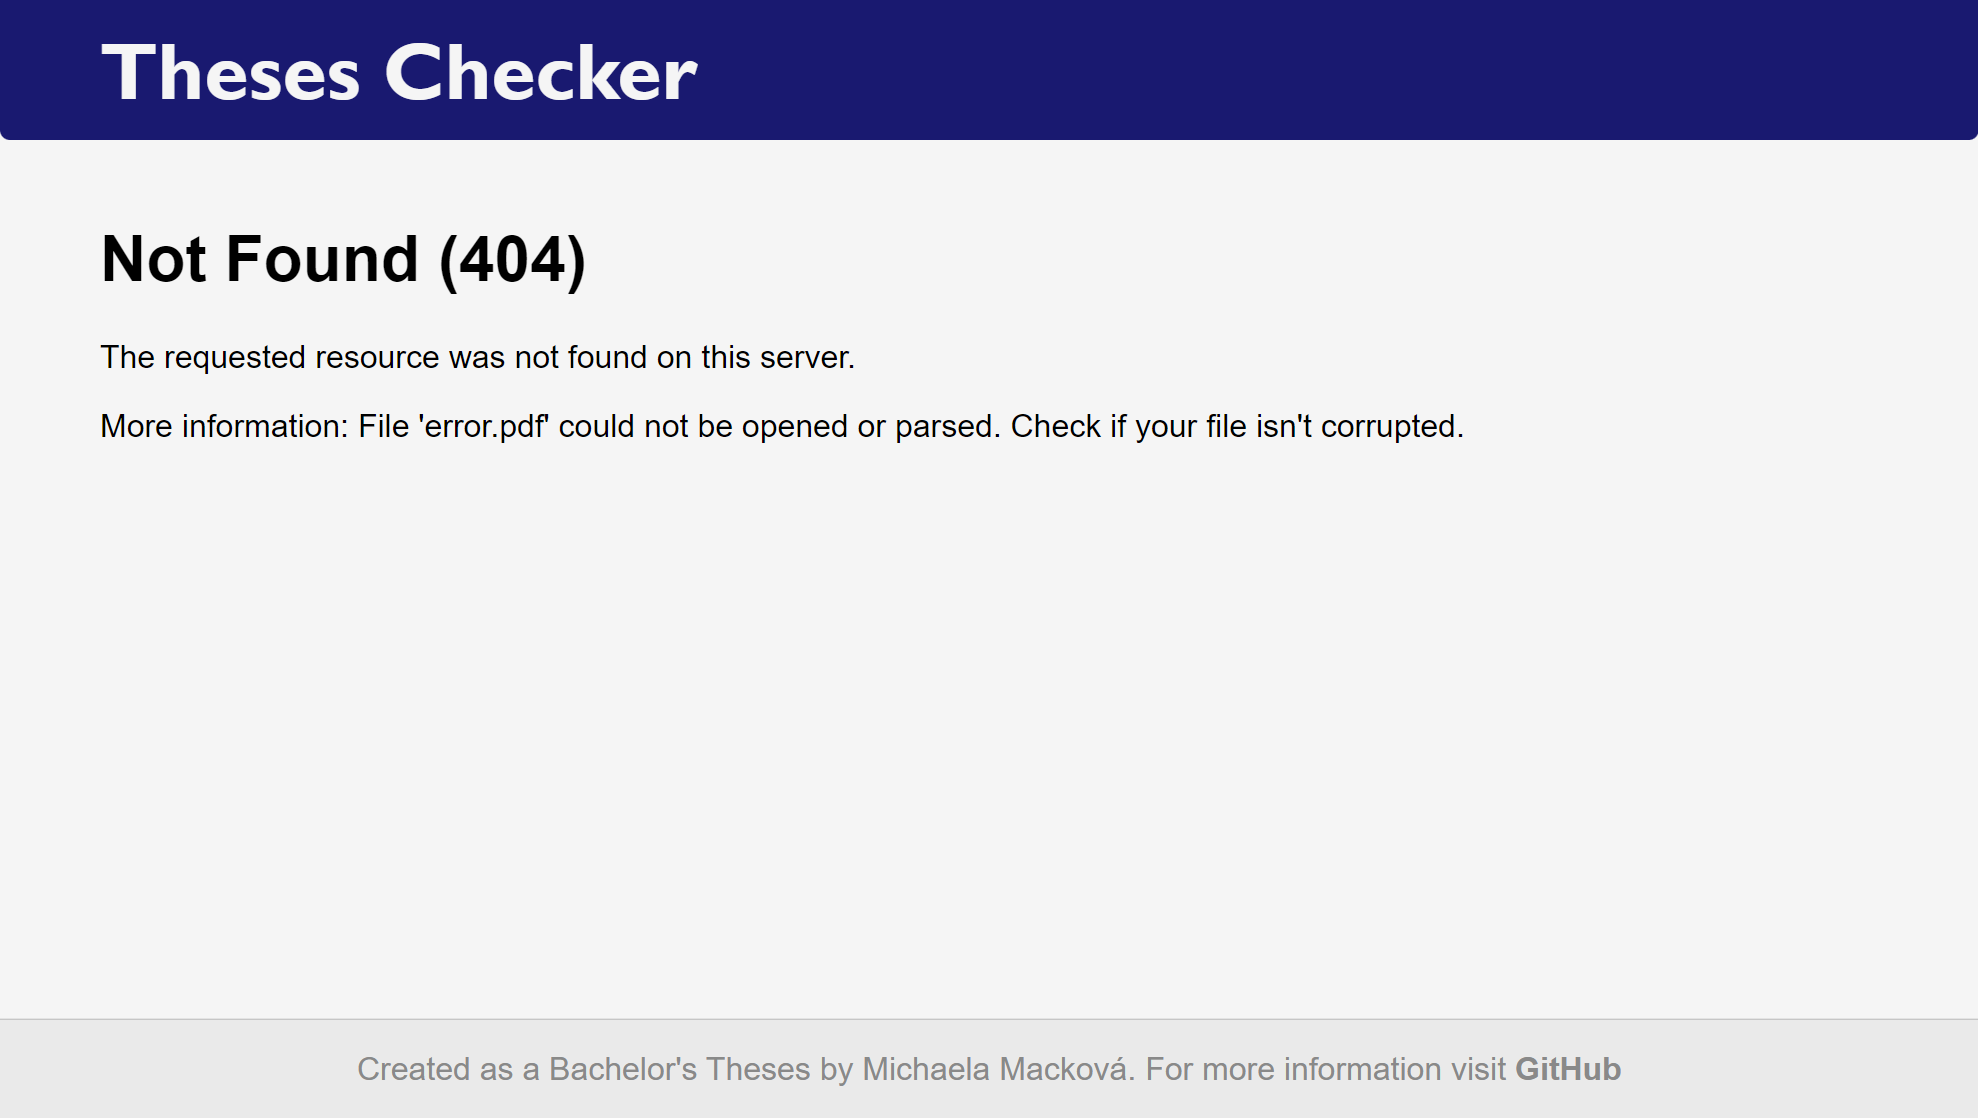
\includegraphics[width=\linewidth]{obrazky-figures/screenshot-error.png}
    \caption{
        Na tomto obrázku je ukázka stránky, která se zobrazí při pokusu o~zpracování
        PDF souboru, který nelze otevřít
    }
    \label{pic_theses_checker_error}
\end{figure}



%#######################    4.5 Program pro použití v~příkazovém řádku    #######################
\section{Program pro použití v~příkazovém řádku}

Implementovaná webová aplikace umí najednou kontrolovat pouze jeden nahraný PDF
soubor. Vedoucí diplomových prací často potřebují zkontrolovat více takových
souborů, proto byl navíc vytvořen program použitelný v~příkazovém řádku. 
Tento program je v~souboru \texttt{check.py} a~používá program ze
sekce~\ref{checker}. Pro správnou funkčnost musí být tyto dva soubory uloženy ve
stejné složce. Program umí na jeden příkaz kontrolovat více PDF souborů
a~s~pomocí nepovinných přepínačů \texttt{-o}, \texttt{-i}, \texttt{-H}, 
\texttt{-t}, \texttt{-s}, \texttt{-e} a~\texttt{-b} lze určit, které kontroly
budou či nebudou probíhat. Tento script podporuje navíc nepovinný přepínač
\texttt{-{-}embedded\_PDF}, který určuje, zda budou vnořené PDF brány jako
vektorové obrázky. Ukázky použití lze vidět na 
obrázku~\ref{pic_theses_checker_cmd}.

\begin{figure}[H]
    \centering
    \begin{subfigure}[b]{0.8\linewidth}
        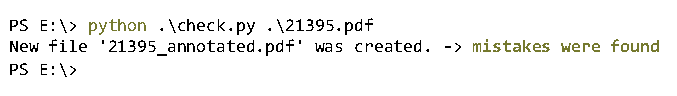
\includegraphics[width=\linewidth]{obrazky-figures/cmd_screenshot_one.pdf}
        \caption{Ukázka spuštění všech kontrol pro jeden PDF soubor}
        \label{pic_theses_checker_cmd_one}
    \end{subfigure}

    \hfill\\
    \begin{subfigure}[b]{0.85\linewidth}
        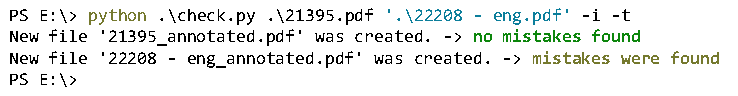
\includegraphics[width=\linewidth]{obrazky-figures/cmd_screenshot_many.pdf}
        \caption{Ukázka spuštění pouze dvou kontrol na dvou PDF souborech}
        \label{pic_theses_checker_cmd_many}
    \end{subfigure}
    \caption{
        Tyto obrázky ukazují možné použití programu Theses Checker
        z~příkazového řádku
    }
    \label{pic_theses_checker_cmd}
\end{figure}



\subsection*{Závislosti}
Aby mohla být aplikace použitelná potřebuje následující:
\begin{itemize}
    \item Python\,==\,3.10.7
    \item PyMuPDF\,==\,1.20.2
    \item numpy\,==\,1.23.5
\end{itemize}
Jiné verze těchto závislostí nebyly testovány.



%#######################    4.6 Implementace programu pro vyhledání chyb a~jejich následné vyznačení    #######################
\section{Implementace programu pro vyhledání chyb a~jejich následné vyznačení} \label{checker}
Program, který zodpovídá za práci s~PDF dokumentem, je obsažen v~souboru s~názvem
\texttt{theses\_checker.py}. Pro zkontrolování technické zprávy se musí použít
funkce \texttt{annotate()} ze třídy \texttt{Checker}. Při vytváření instance této
třídy se musí uvést cesta ke kontrolovanému PDF souboru. Třída \texttt{Checker}
v~sobě obsahuje všechny potřebné metody a~proměnné pro správnou funkci hledání
a~zvýrazňování chyb uvnitř PDF dokumentů.

Třídní proměnné jsou rozděleny do dvou skupin -- statické třídní proměnné
a~třídní proměnné vázané na jednu instanci. Statické třídní proměnné nemění 
svou přiřazenou hodnotu a~třídní proměnné instance naopak během programu
svou hodnotu mění.

Třída \texttt{Checker} obsahuje několik veřejných proměnných a~metod, 
které se používají 
při zpracovávání PDF souboru. Tyto proměnné a~metody lze vidět na 
obrázku~\ref{pic_class_Checker}. Proměnné \texttt{RND\_PAGE\_CNT},
\texttt{HIGHLIGHT\_PADDING} a~proměnné označeny jako \emph{Nastavení barev}
jsou statické třídní proměnné. Tyto proměnné lze nastavit před použitím
funkce \texttt{annotate()}. Proměnné, které jsou označeny jako
\emph{Nastavení barev} jsou využívány především pro jednotnou barvu označení
nalezených chyb. Veřejné třídní proměnné instance jsou proměnné 
\texttt{borderNotFound} a~\texttt{mistakes\_found}. Tyto dvě proměnné
slouží jako pomocný výstup aplikace a~nesou v~sobě informaci o~tom, jak
probíhalo zpracování PDF dokumentu.
\begin{figure}[H]
    \centering
    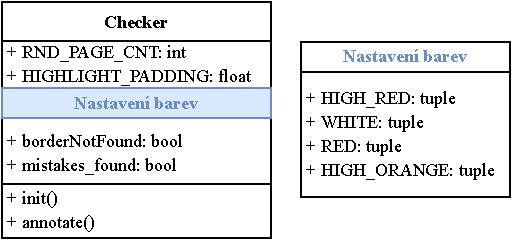
\includegraphics[width=0.7\linewidth]{obrazky-figures/class_Checker.pdf}
    \caption{
        Na tomto obrázku jsou vyznačeny všechny veřejně přístupné proměnné
        a~metody třídy \texttt{Checker}. Proměnné pro nastavení barev jsou
        speciálně vyznačeny
    }
    \label{pic_class_Checker}
\end{figure}
Každá z~těchto veřejných proměnných plní vlastní funkci. Statické třídní
proměnné se používají pro:
\begin{itemize}
    \item \texttt{RND\_PAGE\_CNT}\,--\,Tato proměnná se používá při zjišťování
    základních informací o~dodaném PDF dokumentu. Tyto informace jsou potřebné
    pro správné hledání chyb. Proměnná obsahuje maximální počet náhodných stran,
    které jsou zkoumány pro získání těchto základních informací.

    \item \texttt{HIGHLIGHT\_PADDING}\,--\,Tato proměnná obsahuje velikost okraje,
    který je použit, když je zvýraznění moc těsné zvýrazněnému objektu. Toto
    nastává při hledání přetečení okraje stránky.

    \item \texttt{HIGH\_RED}\,--\,Proměnná obsahuje červenou barvu pro zvýraznění
    textu při nalezené chybě. Barva je ve formátu RGB\footnote{
        Knihovna PyMuPDF umí pracovat s~několika různými formáty barev, jako
        jsou například formáty CMYK, GRAY, RGB a~sRGB. 
        Formát RGB je uspořádaná trojice, kde každý prvek obsahuje celé číslo
        v~intervalu $\left\langle 0;255 \right\rangle$.
    }.

    \item \texttt{WHITE}\,--\,Proměnná obsahuje bílou barvu ve formátu RGB 
    a~je považována jako barva pozadí PDF stránky. 
    
    \item \texttt{RED}\,--\,Je to červená barva ve formátu RGB. Tato barva je
    použita při kreslení přímek.
    
    \item \texttt{HIGH\_ORANGE}\,--\,Je to oranžová barva ve formátu RGB pro
    zvýraznění textu při varování. 
\end{itemize}
Veřejné třídní proměnné instance mají funkci:
\begin{itemize}
    \item \texttt{borderNotFound}\,--\,Tato proměnná je veřejná a~označuje, zda byl
    při hledání základních informací o~dokumentu nalezen okraj stránky.

    \item \texttt{mistakes\_found}\,--\,Veřejná proměnná typu boolean, která označuje,
    zda byla při kontrole PDF dokumentu nalezena jakákoliv chyba (či varování
    na chybu).
\end{itemize}



Dále třída \texttt{Checker} obsahuje privátní třídní proměnné instance
a~privátní metody. 
Některé privátní proměnné jsou využívány pro navigaci v~kontrolovaném dokumentu
a~další v~sobě mají o~tomto dokumentu uložená data, která jsou potřebná
k~prováděným kontrolám. Tyto privátní proměnné jsou vyznačeny na
obrázku~\ref{pic_class_Checker_private}. 
\begin{figure}[H]
    \centering
    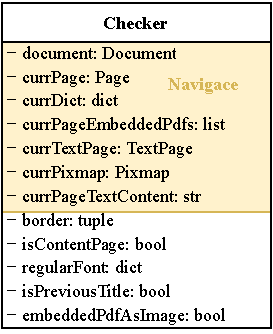
\includegraphics[width=0.4\linewidth]{obrazky-figures/class_Checker_private.pdf}
    \caption{Tento obrázek ukazuje všechny privátní proměnné třídy \texttt{Checker}}
    \label{pic_class_Checker_private}
\end{figure}
Privátní proměnné, které se používají pro navigaci v~dokumentu, jsou:
\begin{itemize}
    \item \texttt{\_\_document}\,--\,Tato proměnná obsahuje instanci
    kontrolovaného PDF dokumentu.

    \item \texttt{\_\_currPage}\,--\,Toto je proměnná, která obsahuje instanci
    aktuálně zpracovávané strán\-ky z~PDF dokumentu.

    \item \texttt{\_\_currDict}\,--\,Tato proměnná obsahuje aktuálně
    zkoumanou stránku ve formě slovníku, jehož struktura je uvedena na
    obrázku~\ref{pic_curr_page_dict}, ve kterém je označen jménem \emph{Stránka}.
    \begin{figure}[H]
        \centering
        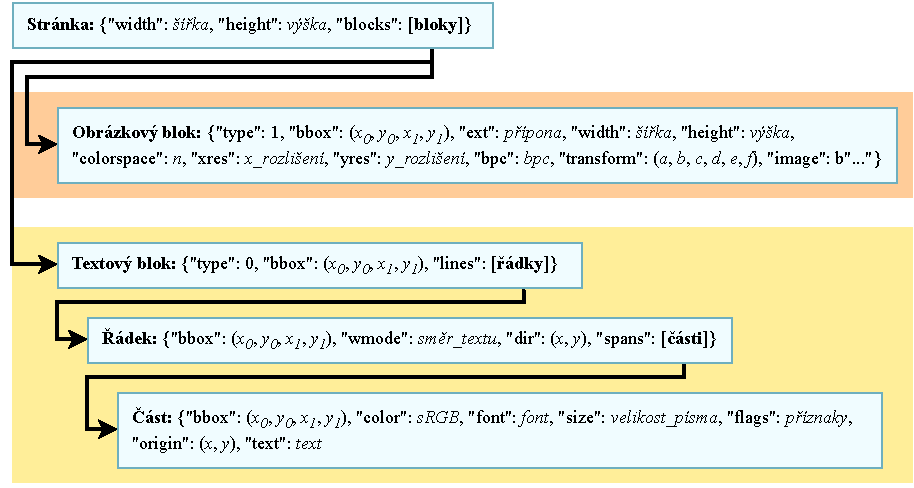
\includegraphics[width=\linewidth]{obrazky-figures/page_dictionary.pdf}
        \caption{
            Na tomto obrázku je vyznačena struktura slovníku \texttt{\_\_currDict}.
            Obrázek byl převzat a~upraven z~oficiální PyMuPDF 
            dokumentace~\cite[Sekce: \emph{TextPage}]{PyMuPDF} 
            }
        \label{pic_curr_page_dict}
    \end{figure}

    \item \texttt{\_\_currPageEmbeddedPdfs}\,--\,Toto je proměnná, která obsahuje
    seznam vykreslených vložených PDF na aktuálně zpracovávané stránce. Každá
    položka tohoto seznamu je pro kompatibilitu s~proměnnou \texttt{\_\_currDict}
    typu slovníku, který odpovídá slovníku \emph{Obrázkový blok} uvedeném na
    obrázku~\ref{pic_curr_page_dict}. 
    
    \item \texttt{\_\_currTextPage}\,--\,Tato proměnná obsahuje instanci
    takzvané \emph{textpage} aktuálně zpracovávané stránky. Textpage se používá
    pro urychlení některých funkcí pracující s~PDF stránkou.
    
    \item \texttt{\_\_currPixmap}\,--\,Tato proměnná obsahuje takzvanou pixelovou
    mapu aktuálně skenované stránky. Pixelová mapa je podobná obrázku a~v~tomto
    programu se používá pouze pro nalezení přetékajících objektů za okraje
    aktuálně kontrolované stránky.
    
    \item \texttt{\_\_currPageTextContent}\,--\,Tato proměnná obsahuje
    všechen text vyskytující se na aktuální stránce. Jelikož při extrakci textu
    z~PDF stránky nelze vždy získat nepřerušovaný text (text většinou obsahuje
    například znak zalomení řádku tam, kde by byl vykreslen na stránce), 
    musí se nejdříve tento extrahovaný text upravit.
    Text obsažen uvnitř proměnné \texttt{\_\_currPageTextContent} je formátován
    přímo pro čtení, což znamená, že znaky nového řádku, které byli přidány pro správné 
    zobrazení na PDF stránce, jsou nahrazeny za mezeru a~jsou odebrány
    spojovníky u~rozdělených slov (např. \emph{spojo-vník}). Každý blok textu
    vyskytnutý na PDF stránce je v~této proměnné
    oddělen prázdným řádkem. 
\end{itemize}
Privátní proměnné, které uchovávají informace pro prováděné kontroly, jsou: 
\begin{itemize}
    \item \texttt{\_\_border}\,--\,Tato proměnná obsahuje nalezené souřadnice 
    levého a~pravého okraje stránky.
    \item \texttt{\_\_isContentPage}\,--\,Tato proměnná
    označuje, zda aktuální stránka je stránka obsahu.
    \item \texttt{\_\_regularFont}\,--\,Tato proměnná obsahuje
    font, který je ve zpracovávaném dokumentu použit pro klasický text.
    \item \texttt{\_\_isPreviousTitle}\,--\,Toto je pomocná proměnná pro
    kontrolu chybějícího textu mezi nadpisy. V~této proměnné je uloženo,
    zda předchozí blok textu byl nadpis.
    \item \texttt{\_\_embeddedPdfAsImage}\,--\,Tato proměnná určuje, zda se
    má s~vnořenými PDF soubory pracovat jako s~obrázkem, či nikoliv.
\end{itemize} 

Než se budou moct provézt některé kontroly, musí se nejdříve zjistit pár
základních informací o~kontrolovaném dokumentu (například font normálního textu
nebo souřadnice okrajů stránek). Toto získávání informací provádí funkce
\texttt{\_\_getDocInfo()}, která pro zrychlení programu skenuje pouze předem
určený počet stran. Skenované stránky jsou získány náhodně.

Hlavní funkce \texttt{annotate()} (naznačená ve výpisu~\ref{code_annotate}) přijímá parametry typu boolean, kde
každý typ kontroly má vlastní parametr. Tyto parametry určují, zda se má daná
kontrola provést, či nikoliv. Další parametry, které tato funkce přijímá jsou
\texttt{annotatedPath}, který určuje cestu pro vytvořený anotovaný soubor,
a~\texttt{embeddedPdfAsImage}, který je typu boolean a~označuje, zda se mají
při kontrolách chovat vložené PDF soubory jako obrázky, nebo jako pokračování
daného PDF dokumentu. Tato funkce provádí všechny kontroly a~vše s~nimi spojené.
To znamená zjištění potřebných informací, samotná kontrola a~označení nalezených
chyb. Každá kontrola má vlastní funkci, která prozkoumá jednu stránku a~nalezené
chyby označí pomocí PDF anotací (vysvětleny v~sekci~\ref{PDF_annotations}).
Chyby, které program umí zkontrolovat, jsou přetečení za okraj stránky, 
špatné použití spojovníku, nevhodná šířka obrázku, vynechaná mezera před levou
závorkou, chybějící text mezi názvy sekcí a~odkaz na neexistující referenci.

\noindent\begin{minipage}{\linewidth}
    \hfill
    \lstinputlisting[style=myPython,caption={
        V~tomto výpisu je naznačena veřejná funkce \texttt{annotate()},
        která provede všechny kontroly a~uloží anotovaný soubor
    },label=code_annotate]{code_examples/python_code/annotate.py}
\end{minipage}


%---------- 4.6.1 Nalezení okraje stránky ----------
\subsection*{Nalezení okraje stránky}
Hlavní kontrola, na kterou se měl tento program zaměřit, je přetékání objektů za
okraj stránky. Pokud jsou známy souřadnice okraje, nalezení jeho přetečení
se řídí algoritmem naznačeném ve výpisu~\ref{code_overflow}.

\noindent\begin{minipage}{\linewidth}
    \hfill
    \lstinputlisting[
        style=myPython, caption={
            Výpis naznačuje funkci \texttt{getOverflow()}, která získá souřadnice 
            všech přetečení okraje stránky
        }, label=code_overflow
    ]{code_examples/python_code/overflow.py}
\end{minipage}

PDF dokument nemusí mít uloženou informaci o~souřadnicích okraje stránky. Pro
jeho nalezení se tak musí daná informace nalézt z~již vykreslené stránky.
Použitá knihovna PyMuPDF obsahuje funkce, díky kterým lze zjistit polohu
vykreslených objektů a~podobjektů (například obrázků, bloků textu a~řádků v~nich
obsažených). Pokud blok textu obsahuje přetečení, ohraničení celého bloku
obsahuje i~toto přetečení (viz obrázek~\ref{pic_block_bbox}).

\begin{figure}[H]
    \centering
    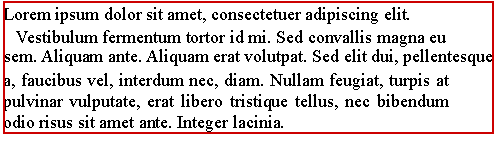
\includegraphics[width=0.7\linewidth]{obrazky-figures/block_bbox.pdf}
    \caption{Obrázek ukazuje červeně označené ohraničení bloku textu, který obsahuje přetečení}
    \label{pic_block_bbox}
\end{figure}

Při hledání okraje stránky je použitý algoritmus inspirován tím, jak takový
okraj hledá člověk. Prozkoumá se každý řádek textu, který se vyskytuje na
stránce a~uloží se souřadnice jeho levého i~pravého okraje. Za okraj stránky se
poté považuje medián těchto uložených okrajů řádků. První řádek v~odstavci 
může být odsazený, a~proto se pro větší přesnost tohoto algoritmu (uvedeného
ve výpisu~\ref{code_get_page_border}) neukládá do potenciálních levých okrajů.
Podobné pravidlo platí i~pro poslední řádek a~jeho pravý okraj.

\noindent\begin{minipage}{\linewidth}
    \hfill
    \lstinputlisting[style=myPython, caption={
        Výpis naznačuje funkci \texttt{getPageBorder()}, která nalezne
        levý a~pravý okraj stránky
    }, label=code_get_page_border]{code_examples/python_code/getPageBorder.py}
\end{minipage}
 

%---------- 4.6.2 Nalezení souřadnic vloženého PDF na stránce ----------
\subsection*{Nalezení souřadnic vloženého PDF na stránce}
V~technické zprávě se často vyskytují obrázky. Jak je řečeno 
v~podkapitole~\ref{vector_graphic}, je vhodné používat vektorovou grafiku
pro grafy a~schémata. Vektorové obrázky mohou mít formát PDF, a~ty se poté
vkládají do PDF dokumentu technické zprávy. Při zpracovávání tohoto PDF dokumentu
se nijak nerozlišuje mezi interními částmi původního PDF dokumentu a~vloženého
PDF obrázku. Kontroly určené pro obrázky tedy nezahrnují tyto vložené PDF
a~kontroluje se pouze text uvnitř těchto obrázků.

Aby se s~vloženým PDF mohlo pracovat jako s~obrázkem, musí se zjistit
jeho poloha na stránce. Ve formátu PDF nejsou nikde přímo uvedeny souřadnice
vloženého PDF obrázku. Obrázek ve formátu PDF je uvnitř PDF dokumentu uložen
jako XObject (popsaný v~podkapitole~\ref{XObject}) a~jak je na dané stránce
vykreslen je popsáno v~toku content stream (více lze nalézt
v~sekci~\ref{content_streams}) té stejné stránky.
Pro zjištění souřadnic vykresleného obrázku tedy program simuluje
stavy datové struktury graphics state, jenž je popsána
v~podkapitole~\ref{graphics_state}. Přesněji stačí simulovat parametr
CTM (current transformation matrix), ve kterém je uvedena matice pro transformaci
z~uživatelského prostoru do prostoru zařízení. Podtyp objektu XObject, který se
nejčastěji používá pro PDF obrázky, je typ Form XObject.

Příkazy uvedené
v~content streamu, které ovlivňují, jak bude objekt typu Form XObject vykreslen,
jsou \texttt{q} a~\texttt{Q} (manipulace s~graphics state zásobníkem),
\texttt{cm} (změna parametru CTM) a~\texttt{Do} (příkaz pro vykreslení
objektu XObject). Příkazem \texttt{cm} jsou prováděny elementární transformace
obrázku pro jeho správné napolohování na stránce. Jelikož matice CTM musí vždy
vyjadřovat transformaci z~jednoho prostoru do druhého a~příkazy \texttt{cm}
s~touto maticí manipulují, podle dříve uvedeného
vzorce~\eqref{multiple_matrix_transformations} si dokážeme odvodit
vzorec~\eqref{cm_multiplication}. V~tomto vzorci vyjadřuje matice $CTM$
aktuální hodnotu CTM uložené uvnitř graphics state, $M_{cm}$ 
je matice, kterou vyjadřuje operand použitého příkazu \texttt{cm}
a~matice $CTM'$ je výsledná matice, jejíž hodnota je nově uložena do
CTM parametru datové struktury graphics state.
\begin{equation} \label{cm_multiplication}
    CTM' = M_{cm} \cdot CTM
\end{equation}

Pro získání takových souřadnic obrázku, aby se s~nimi mohlo dále pracovat
ve vytvořeném programu, se získané souřadnice musí ještě transformovat
maticí stránky. Tato matice lze získat přímo jako atribut
\texttt{transformation\_matrix} proměnné \texttt{\_\_currPage}.
Stejného výsledku lze dosáhnout, když před získáním souřadnic obrázku pomocí
vynásobení matice CTM, získáme přímo matici transformace obrázku do našeho
vyžadovaného prostoru. Toto je vyjádřeno
v~rovnici~\eqref{picture_transformation_matrix}, kde $CTM$ je aktuální hodnota
parametru CTM ze struktury graphics state, $M_T$ je matice stránky a~$M_{PT}$
je kombinovaná matice transformace obrázku.
\begin{equation} \label{picture_transformation_matrix}
    M_{PT} = CTM \cdot M_{T}
\end{equation}

Použitý algoritmus pro získání souřadnic všech vnořených PDF objektů
vykreslených na aktuální stránce je naznačen ve vývojovém diagramu na
obrázku~\ref{pic_embedded_pdf_flow_chart}.

\begin{figure}[H]
    \centering
    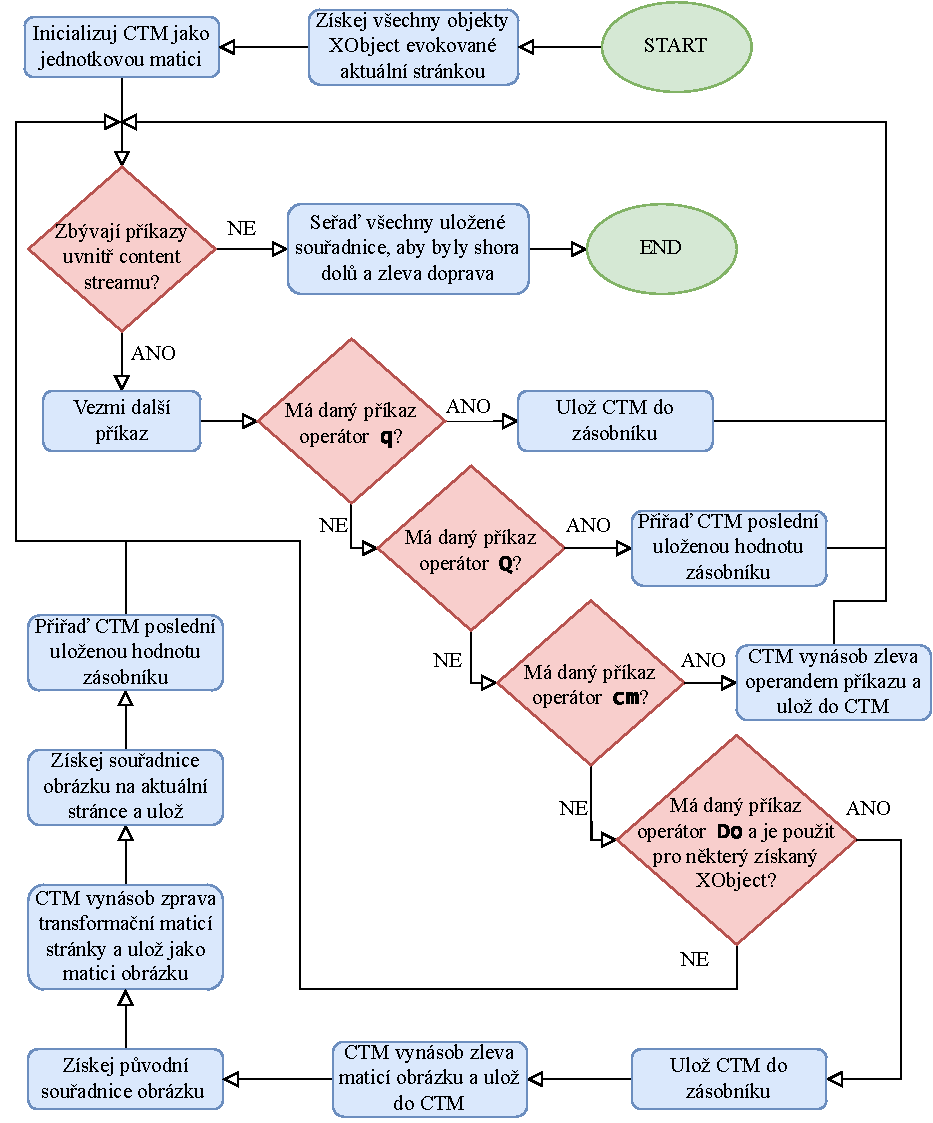
\includegraphics[width=\linewidth]{obrazky-figures/embedded_pdf_flow_chart.pdf}
    \caption{
        Na tomto obrázku je nakreslen vývojový diagram, který popisuje
        algoritmus pro získání souřadnic vnořených PDF. CTM je proměnná imitující 
        CTM (current transformation matrix) z~datové struktury graphics state
        vyskytující se v~PDF. Aktuální stránka je instance PDF stránky, která
        se právě zpracovává a~lze z~ní získat content stream a~vyvolané XObjekty
    }
    \label{pic_embedded_pdf_flow_chart}
\end{figure}


%*********************************************************************************




%*********************************************************************************
%                                 5 TESTOVÁNÍ 
%*********************************************************************************
\chapter{Testování a~zhodnocení výsledné aplikace} \label{testing}
Testování je důležitou součástí vývoje jakéhokoliv nástroje. Během testování
vývojáři dostávají důležitou zpětnou vazbu a~mohou tak být odhaleny chyby,
které je třeba opravit.

Tato kapitola popisuje, jakým způsobem byl testován výsledný nástroj této
bakalářské práce. Jsou zde rozvedeny postupy a~výsledky ověřování funkcionality
vytvořené aplikace. Dále jsou zde zmíněny nedostatky, které se v~této aplikaci
vyskytují a~rozšíření pro budoucí vývoj tohoto nástroje. 



%#######################    5.1 Ověření správné funkcionality vyhledávání chyb    #######################
\section{Ověření správné funkcionality vyhledávání chyb}
Již během prvních funkčních prototypů byla testována přesnost hledání
chyb. Toto testování probíhalo na zveřejněných diplomových pracích, které byly
vytvořeny na Fakultě informačních technologií Vysokého učení technického v~Brně.
Tyto práce byly poskytnuty jako vstupy do programu a~jejich anotované
výstupy byly zkontrolovány ručně. Dále byly tyto výstupy kontrolovány
s~poskytnutými posudky oponenta.

Další vstupní data byla poskytnuta doktorem Tomášem Miletem. Tato data
byly rozpracované práce z~minulých let, které měli doktora Mileta jako
vedoucího. Ke každé takové práci byla vždy poskytnuta její původní forma
a~její upravená forma obsahující poznámky ke zlepšení. Postup testování
na těchto rozpracovaných pracích byl podobný, jako na již zveřejněných, 
jen tyto výstupy z~vytvořené aplikace nebyly porovnávány s~posudkem oponenta,
ale s~poskytnutými poznámkami.



%#######################    5.3 Uživatelské dotazníky    #######################
\section{Uživatelské dotazníky}
Další formou testování bylo provedeno formou dotazníku.
Tento dotazník byl přeposlán několika možným uživatelům
aplikace. Celkově na tento dotazník odpovědělo
34~uživatelů. Dotazník obsahoval tyto otázky:
\begin{itemize}
    \item Pomocí jakého prohlížeče jste aplikaci použili?
    \item Dokázali jste pomocí aplikace Theses Checker zkontrolovat svou
    diplomovou práci?
    \item Dokázali jste jednoduše nahrát PDF soubor?
    \item Zhodnoťte přehlednost označení chyb ve výsledném PDF
    \item Zobrazují se vám pop-up anotace?
    \item Bylo něco špatně označeno jako chyba?
    \item Jaký typ chyby byl špatně označen?
    \item Byla práce s~webovou stránkou jednoduchá?
    \item Máte nějaké nápady na rozšíření či vylepšení?
\end{itemize}

Odpovědi na tento dotazník pomohly vylepšit funkcionalitu vytvořené aplikace.
Hlavním účelem tohoto dotazníku bylo ověření již vytvořených kontrol a~určení,
jak je daná aplikace přehledná. Přehlednost označení nalezených chyb
uvnitř PDF dokumentu mělo většinově dobré ohlasy, což lze
vyčíst i~z~obrázku~\ref{rate_checks}.

\begin{figure}[H]
    \centering
    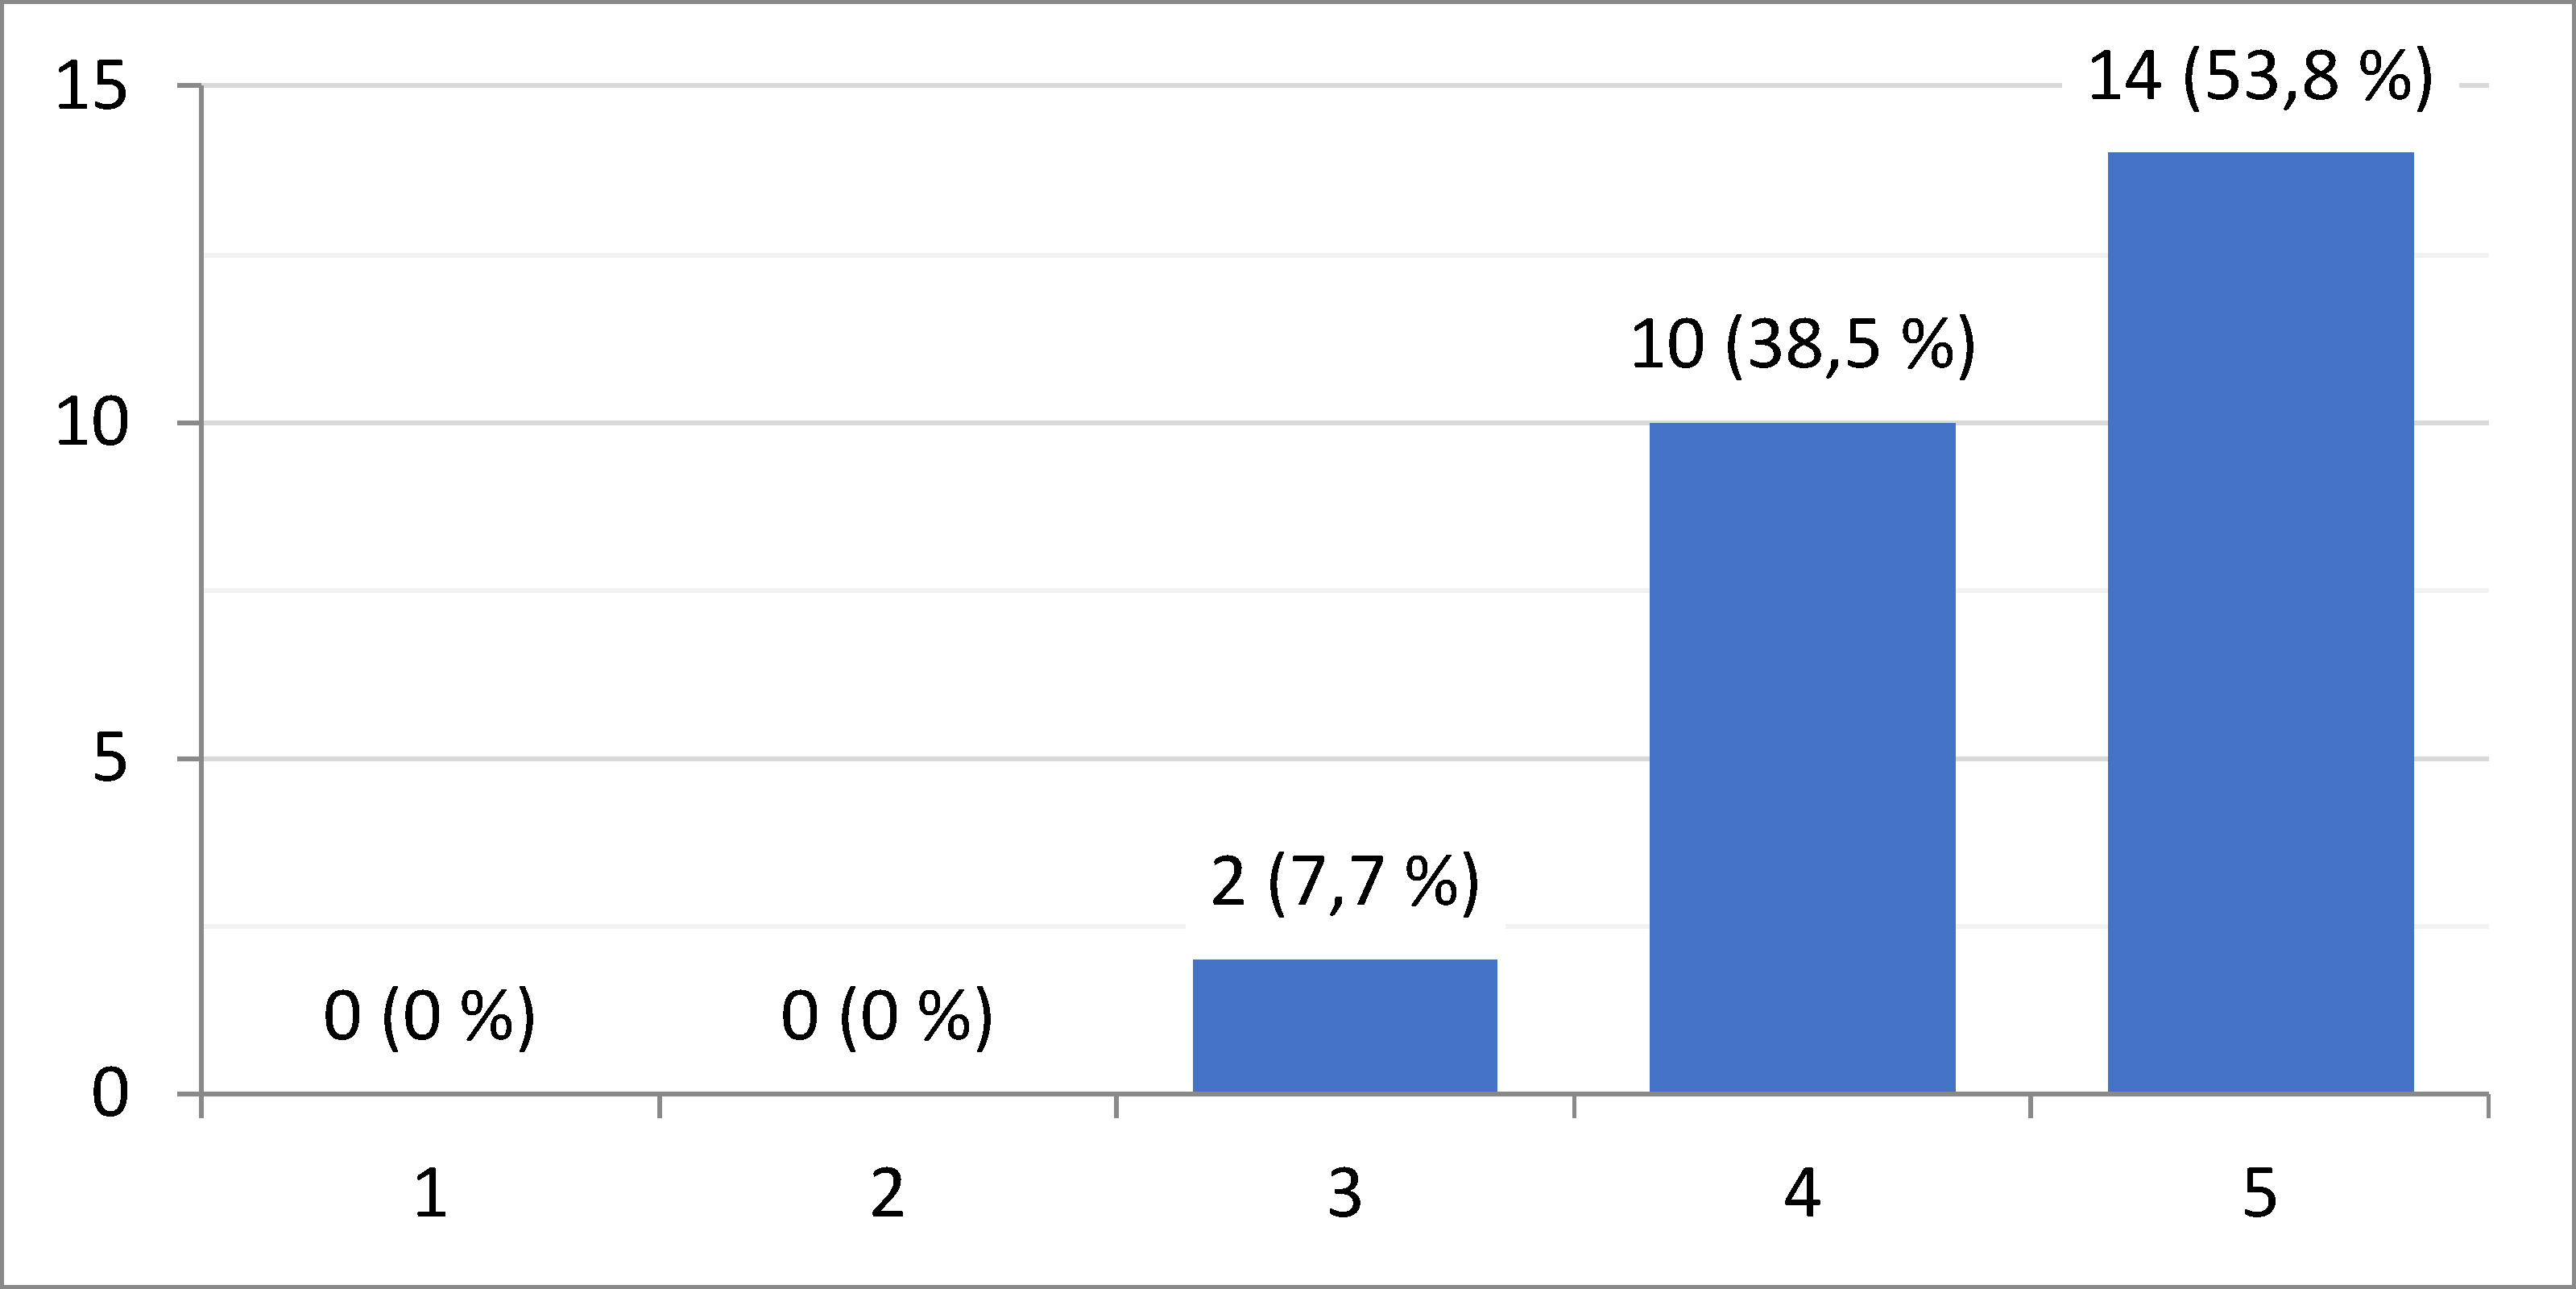
\includegraphics[width=0.8\linewidth]{obrazky-figures/graph1.pdf}
    \caption{
        Obrázek obsahuje graf odpovědí
        na otázku o~přehlednosti označení chyb na stupnici od~1 do~5, kde 
        1~představuje \uv{Zcela nepřehledné}
        a~5~představuje \uv{Jasné}
    }
    \label{rate_checks}
\end{figure}

Ověření funkčnosti kontrol bylo provedeno otázkou na špatné označení chyb
a~upřesněním, který typ chyby byl špatně označen. Shrnutí odpovědí na
první otázku lze vidět na obrázku~\ref{pic_graph_false_mistakes}.
Tento poměr byl očekávaný, jelikož tato testovaná aplikace označuje chyby
false-positive principem.

\begin{figure}[H]
    \centering
    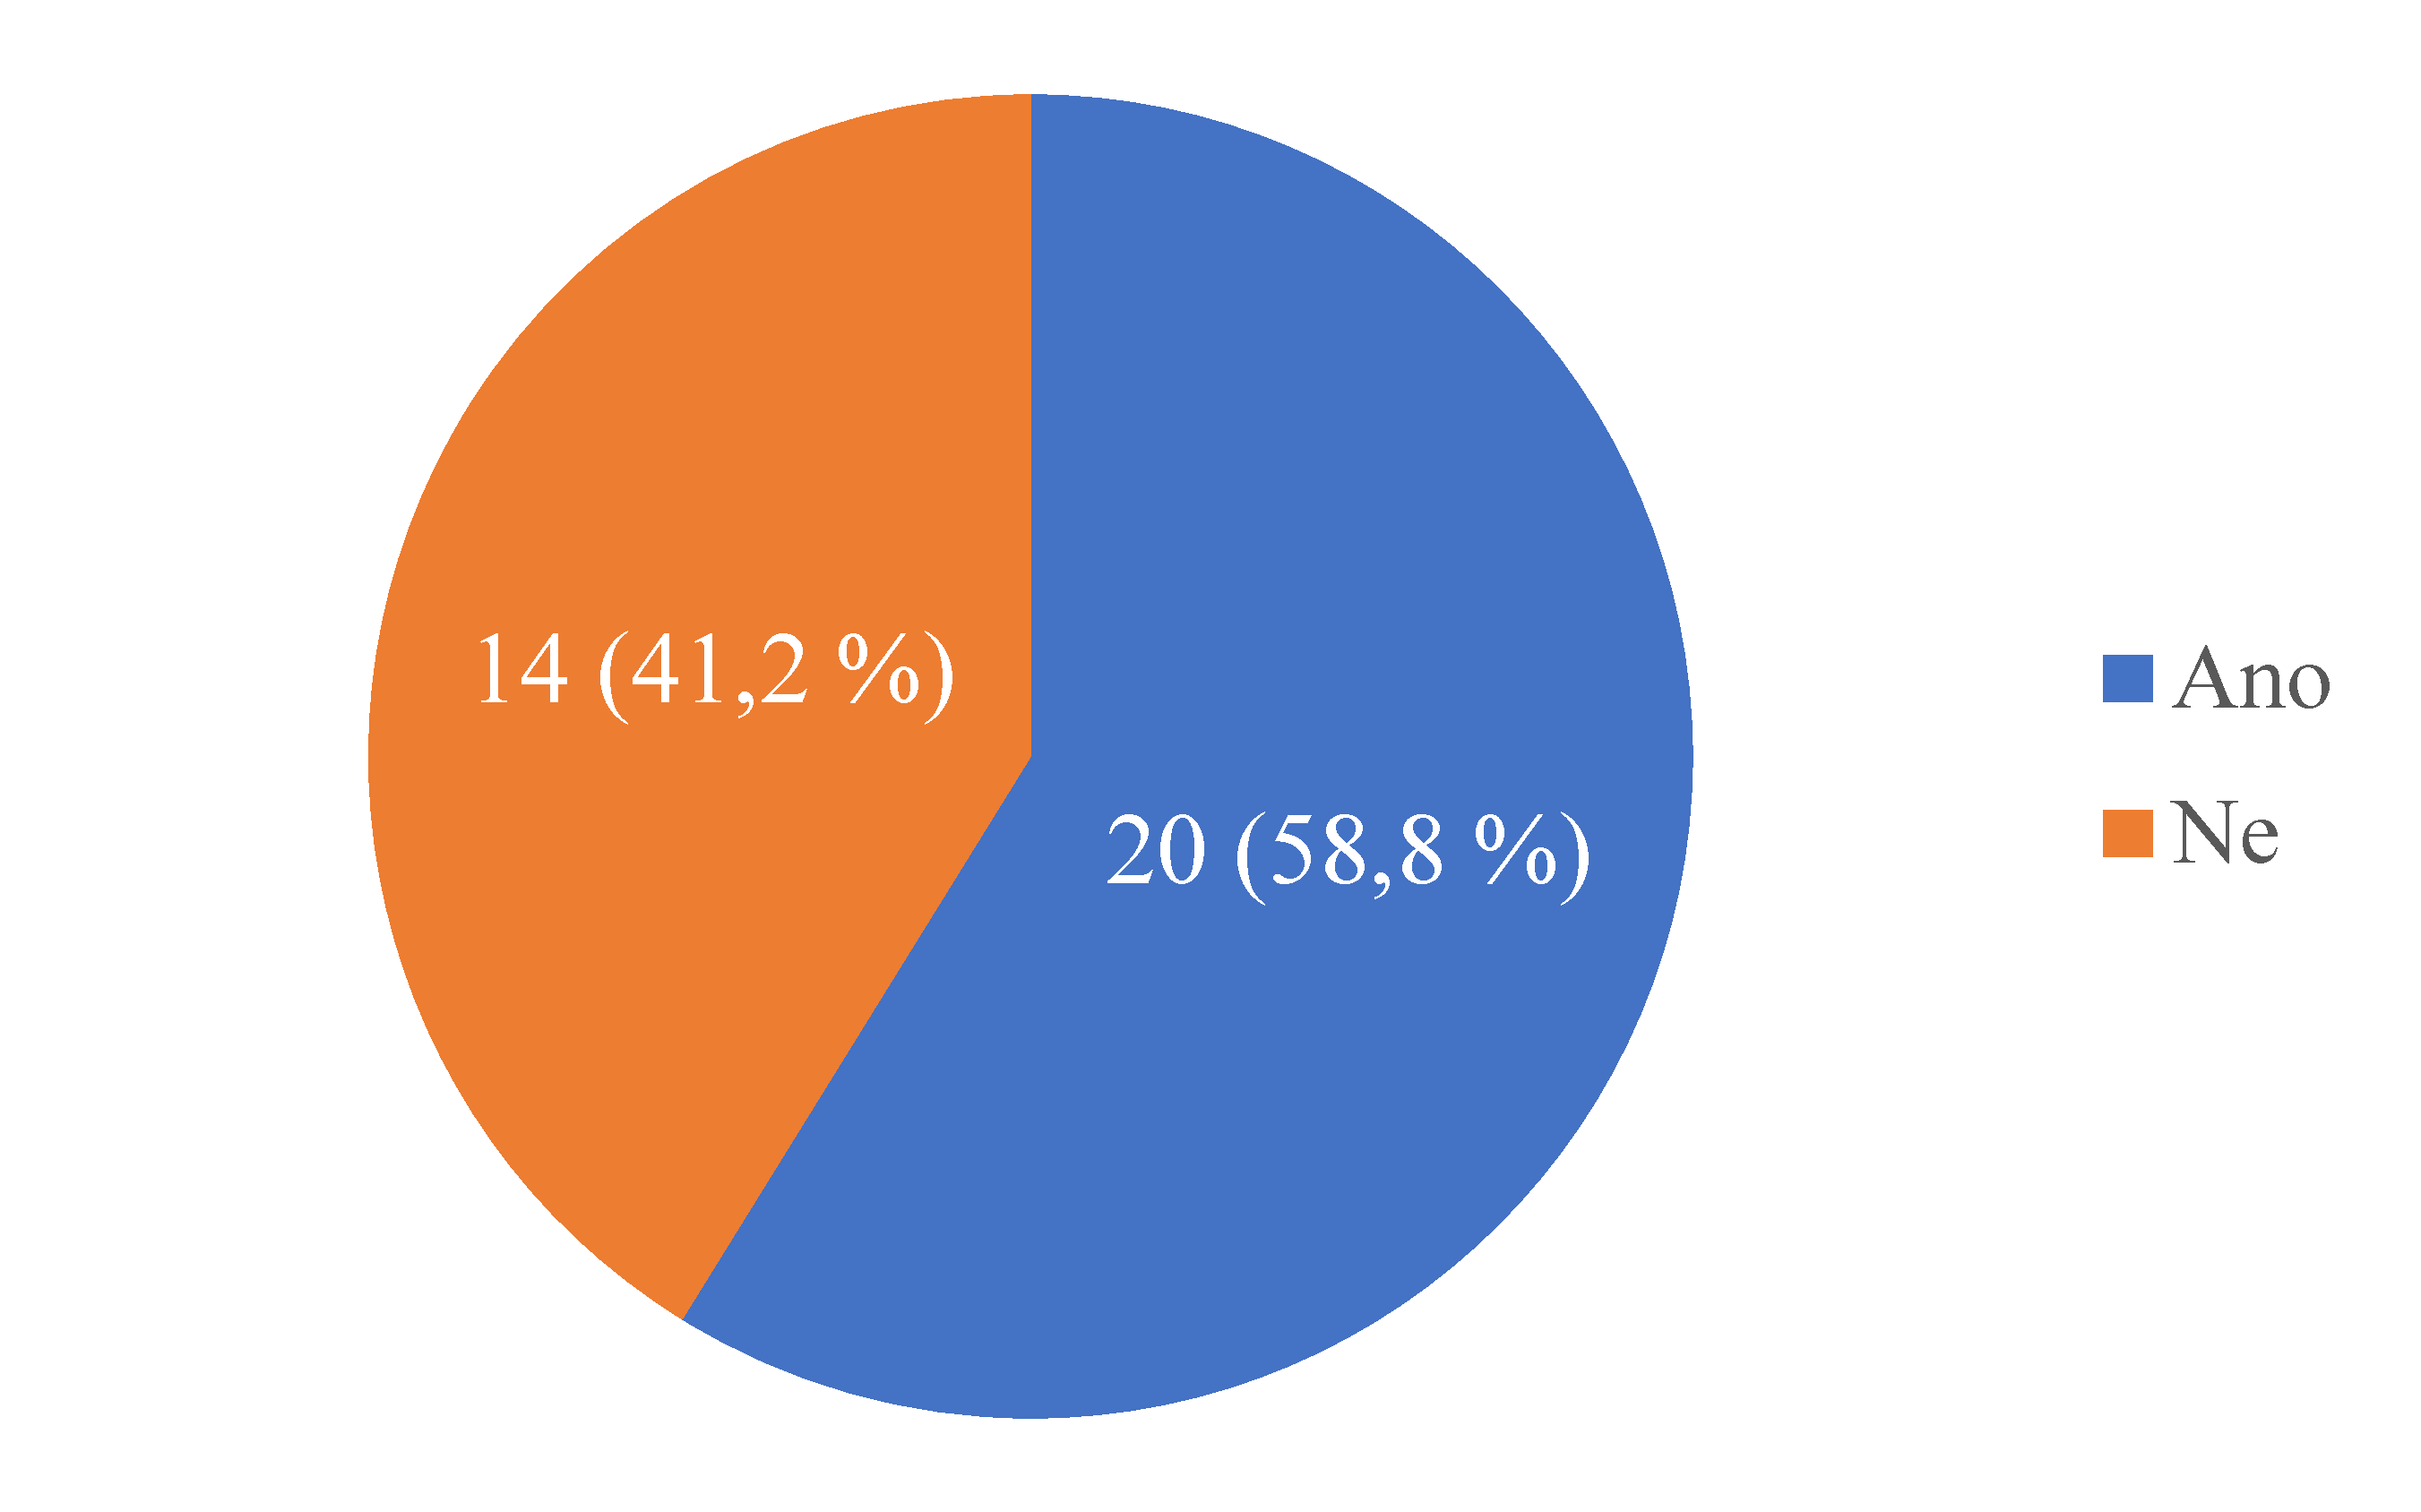
\includegraphics[width=0.6\linewidth]{obrazky-figures/graph_false_mistakes.pdf}
    \caption{
        Tento graf ukazuje shrnutí odpovědí na otázku \uv{Bylo něco špatně označeno jako chyba?}
    }
    \label{pic_graph_false_mistakes}
\end{figure}

Nejčastější špatně označenou chybou byla vynechaná mezera před levou závorkou. 
Celkem tuto chybu uvedlo 12~z~20~(60\,\%)~respondentů a~dále upřesnili, že
toto označení se chybně objevovalo převážně v~matematických vzorcích, u~názvů
funkcí a~ve výpisech kódu. Jako další bylo často zodpovězeno chybné označení
chybějícího textu mezi nadpisy, které se v~odpovědích objevilo celkem~8$\times$.
V~odpovědích bylo upřesněno, že se toto chybné označení objevovalo
okolo tabulek, výpisu kódu a~vektorových obrázků.

Dále byla otestována multiplatformost vytvořené webové aplikace otázkou
na použitý webový prohlížeč. Souhrn odpovědí na tuto otázku je ukázán na
obrázku~\ref{pic_graph_browser}. Zejména takto bylo testováno zobrazení
anotací ve zobrazeném výstupním PDF dokumentu. V~odpovědích na dotazník
byl pouze jediný uživatel, kterému se nezobrazovaly PDF anotace. Tento 
uživatel použil webový prohlížeč Google Chrome.

\begin{figure}[H]
    \centering
    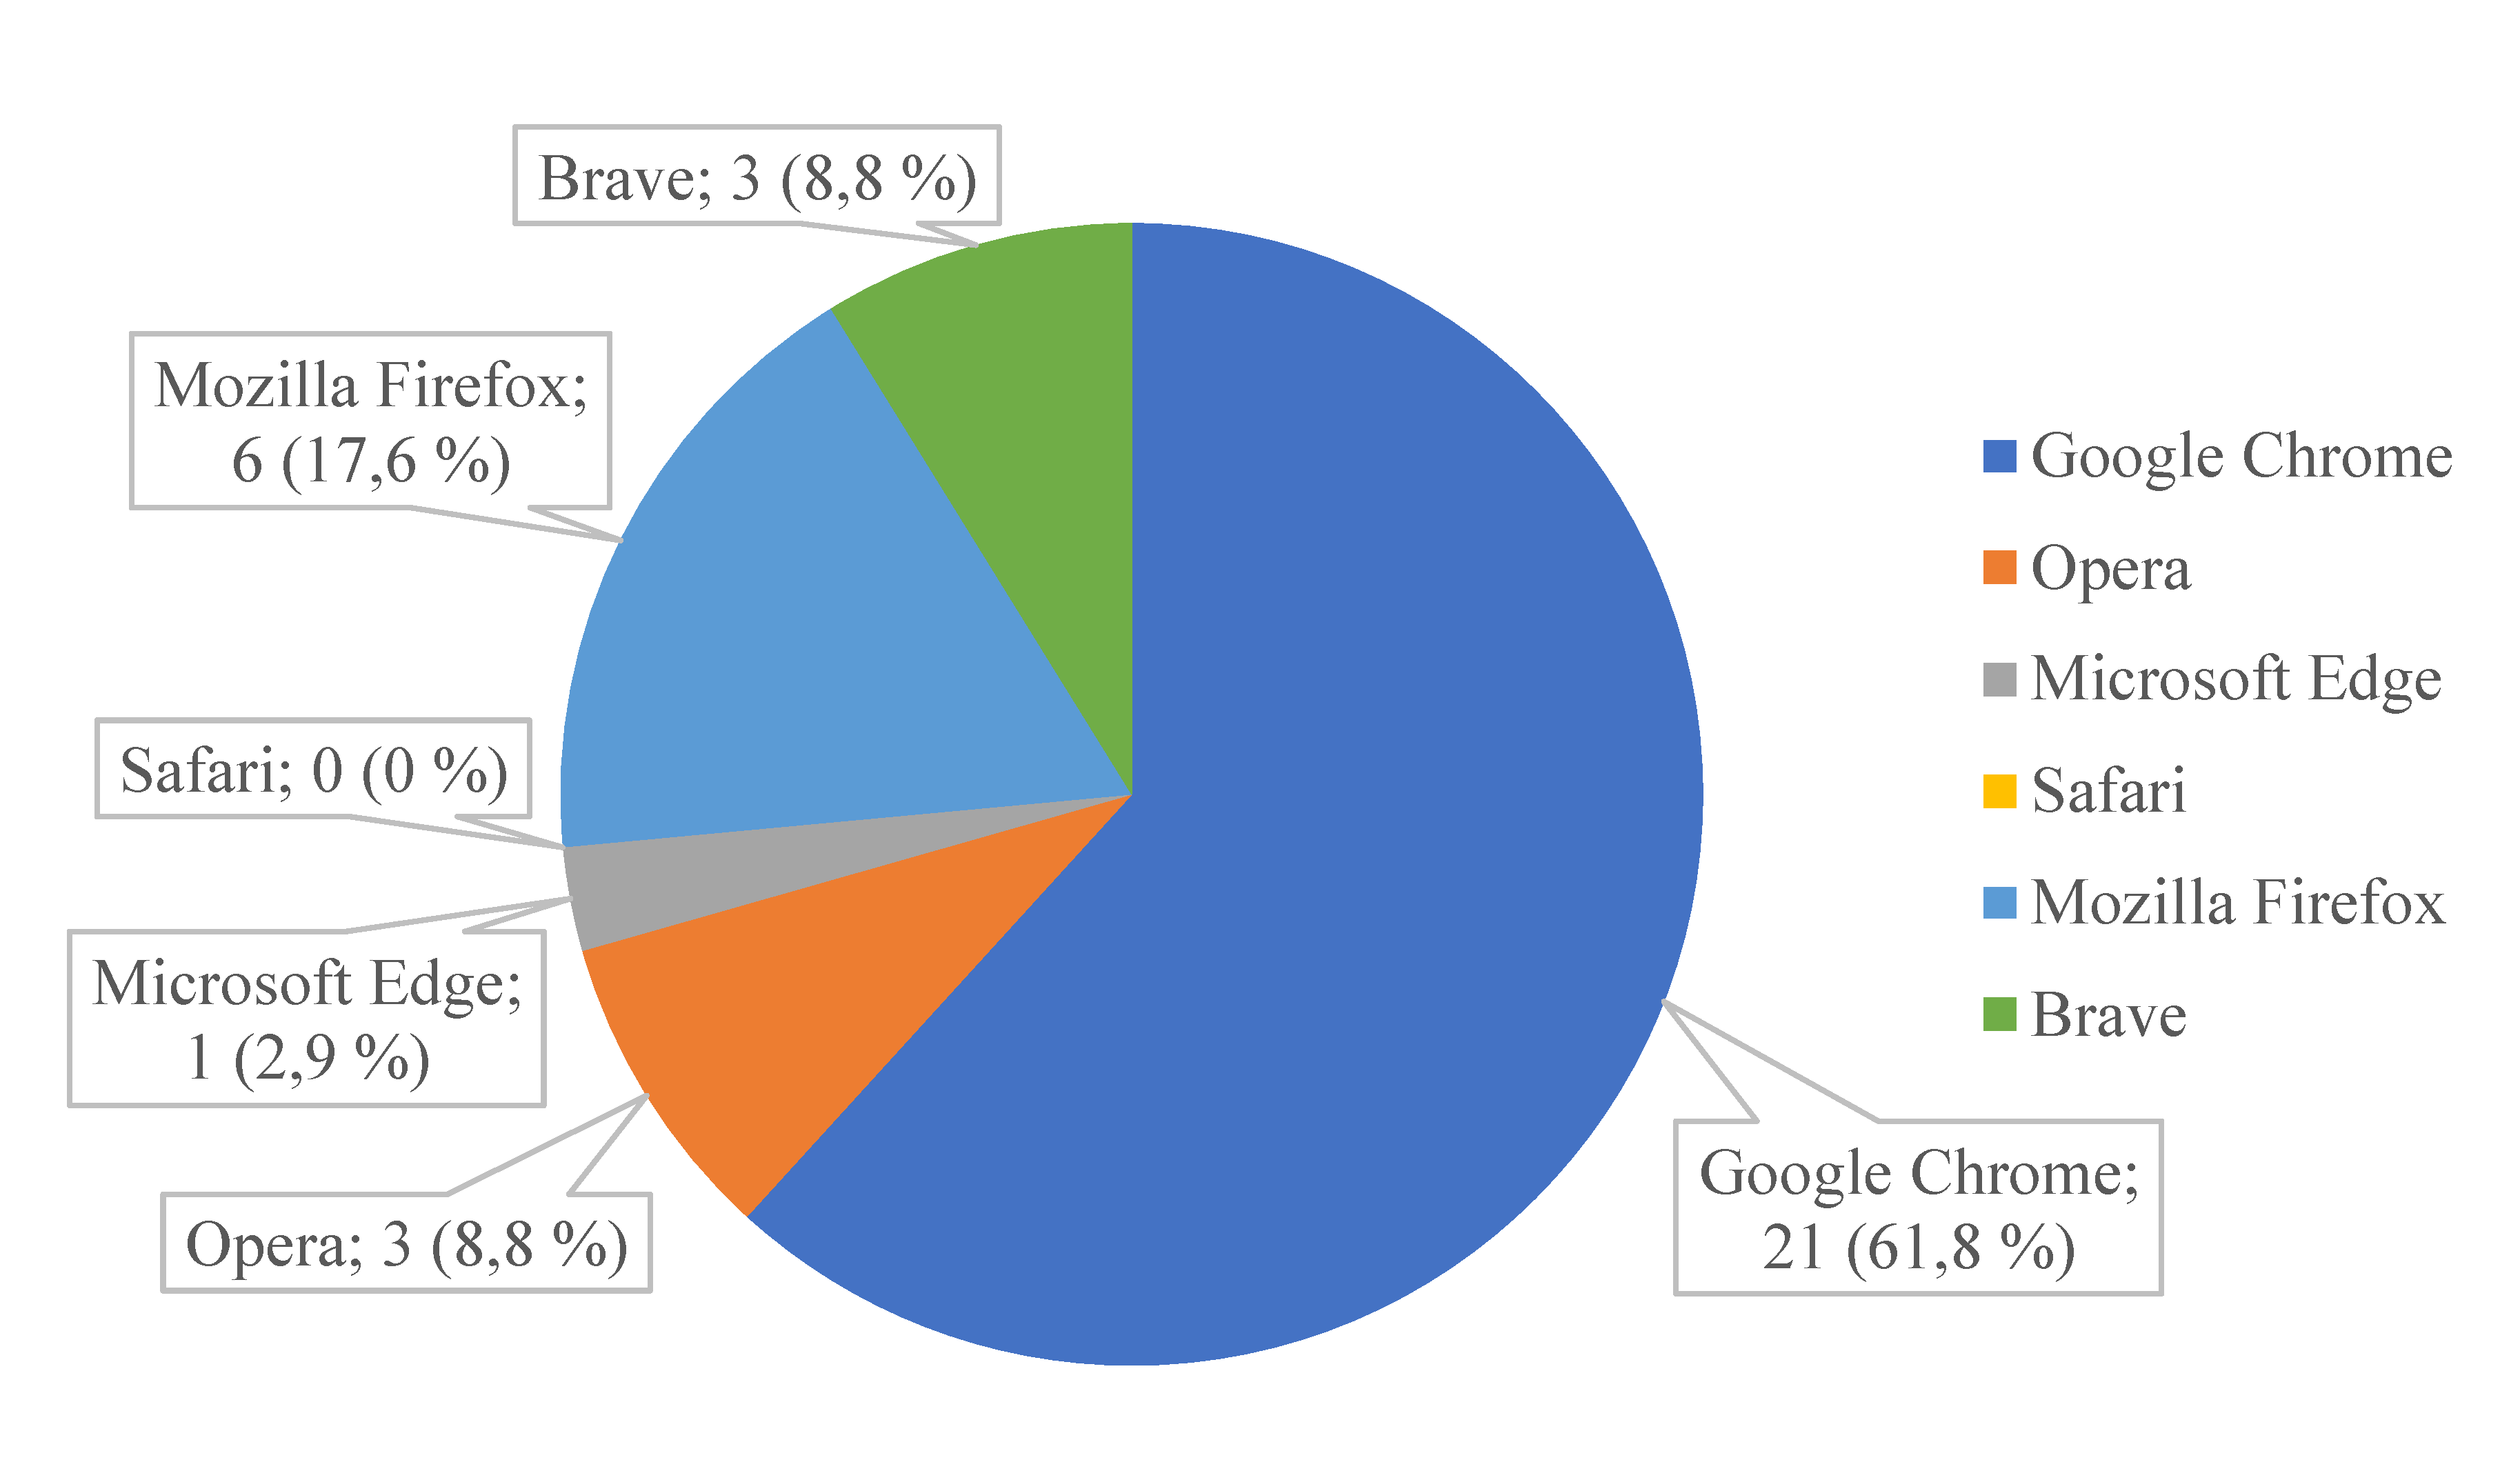
\includegraphics[width=0.85\linewidth]{obrazky-figures/graph_browser.pdf}
    \caption{
        V~tomto obrázku je ukázán graf webových prohlížečů, které byly
        použity uživateli při zkoušení webové aplikace Theses Checker.
        Tyto informace byly získány z~odpovědí na dotazník
    }
    \label{pic_graph_browser}
\end{figure}

Poslední otázka byla nepovinná a~dotazovala se na možné vylepšení webové
aplikace. Některé z~navrhnutých vylepšení jsou:
\begin{itemize}
    \item možnost dát uživateli vypnutí některých kontrol,
    \item na stránce s~výstupem přidat tlačítko na nahrání dalšího PDF souboru,
    \item ukázání seznamu nalezených chyb,
    \item přidání pop-up anotací pro všechny kontroly.
\end{itemize}
Další návrhy byly na přidání nových kontrol, jako jsou například kontroly pro:
\begin{itemize}
    \item krátké sekce,
    \item dlouhé odstavce,
    \item špatnou kvalitu obrázků (rastrové grafy),
    \item citace za odstavcem,
    \item mezeru před odkazem na poznámku pod čarou,
    \item chybějící mezeru před odkazem na kapitolu.
\end{itemize}



%#######################    5.2 Známé chyby aplikace    #######################
\section{Známé chyby aplikace} \label{app_errors}
%Typografická kontrola zahrnuje velmi rozšířenou oblast a~často se váže k~jazyku vypracovaného textu.
Při ověřování správné funkcionality aplikace bylo odhaleno, že vytvořenou webovou aplikaci
nelze použít na mobilním zařízení. Toto je způsobeno načasováním, kdy je odstraněn
výsledný PDF soubor (více viz sekce~\ref{web_app}). Jelikož element
\texttt{<iframe>} neumí na mobilním zařízení zobrazit PDF dokument, nelze tak
získat anotovaný soubor. Při pokusu o~stáhnutí tohoto souboru se pošle dotaz
na server, kde už tento výstupní soubor neexistuje, a~tak je tento vytvořený soubor
nenávratně ztracen.

Během testování bylo objeveno několik dalších nedostatků, které jsou spojeny přímo
s~hledáním chyb. Jelikož se při získávání textu nerozlišuje mezi prostým textem
a~jakýmkoliv jiným elementem obsahujícím text (například grafy a~tabulky),
nalezené nedostatky se nejčastěji objevují právě okolo těchto elementů. 
Jeden takový nedostatek je špatné označení chybějícího popisu kapitoly.
V~tomto případě hraje roli rozeznávání nadpisů, kde text z~tohoto elementu
může být rozpoznán jako nadpis. Dále můžou tyto elementy ovlivnit nalezení
okraje stránky, jelikož texty uvnitř těchto elementů bývají často odsazené.

Dalším často zmiňovaným nedostatkem v~odpovědích na formulář jsou označené
varování na mezeru před levou závorkou na místě, kde se mezera vyskytovat
nemá. Tato místa jsou například názvy funkcí, matematická rovnice a~kód
ve výpisu. Tento nedostatek není lehké opravit, jelikož by pro vylepšení
bylo potřeba poznat kontext textu.



%#######################    5.4 Možné budoucí rozšíření aplikace    #######################
\section{Možné budoucí rozšíření aplikace}
Prvním cílem pro budoucí rozšíření bude přidání zaškrtávacích políček na úvodní
stránce webu pro nastavení kontrol, které se při zpracování provedou. Tato funkce
byla několikrát navrhnuta uživateli jako vylepšení. Jak je uvedeno
v~podkapitole~\ref{app_errors}, některým označením chyb se nedá vyhnout, proto 
bylo navrhnuto, aby bylo možné si zvolit, které kontroly se provedou, a~které se
vynechají.

Další vylepšení se budou týkat samotných kontrol. První vylepšení bude hledání
okrajů pro PDF nastavené na oboustranný tisk. Jelikož u~těchto PDF mají sudé
a~liché stránky jinak nastaveny okraje, nelze v~současném stavu kontrolovat 
přetečení těchto okrajů či další kontroly, které jsou na nalezených okrajích
závislé.

Dalším rozšířením bude přidávání nových kontrol, což je například  kontrola
použití správných uvozovek, detekce jednopísmenných předložek a~spojek na
konci řádku a~kontrola používání vektorových obrázků.



%*********************************************************************************




%*********************************************************************************
%                                   6 ZÁVĚR
%*********************************************************************************
\chapter{Závěr}
Cílem této bakalářské práce bylo vytvořit lehce dostupnou aplikaci, která zpracuje
nahraný PDF dokument a~pomocí PDF anotací v~něm vyznačí nalezené chyby. Tato
aplikace byla vytvořena jako webový nástroj a~nyní je veřejně
přístupná pod názvem Theses Checker\footnote{Theses Checker je dostupný na adrese
\href{https://theseschecker.eu.pythonanywhere.com/}{https://theseschecker.eu.pythonanywhere.com/}}.

Nejdříve bylo zapotřebí zjistit, které chyby se nejčastěji vyskytují v~závěrečných
pracích. Ty byly nalezeny zkoumáním zveřejněných textů a~posudků diplomových prací
vytvořených na Fakultě informačních technologií Vysokého učení technického v~Brně.
Poté byly zkoumány některé dostupné aplikace pro kontrolu textu. Bylo zjištěno,
že žádná dosavadní aplikace se nezaměřuje na typografickou stránku textu, jelikož
se většinou zaměřují na gramatiku.

Další na řadě bylo navrhnutí vzhledu aplikace a~označení nalezených chyb.
V~návrhu a~implementaci byla kladena velká váha na přívětivost pro uživatele.
Aplikace se postupně měnila i~na základě zpětné vazby od uživatelů, která byla
podávána pomocí dotazníku.

Vytvořený program umí kontrolovat šest typů chyb, a~to přetečení za okraj stránky, 
špatné použití spojovníku, nevhodná šířka obrázku, vynechaná mezera před levou
závorkou, chybějící text mezi názvy sekcí a~odkaz na neexistující referenci.
Tento program je využit ve výsledné webové aplikaci a~též pro něj byl 
vytvořen program pro jeho spuštění v~příkazovém řádku.
Výsledky této práce byly představeny na konferenci Excel@FIT. Pro
účast na této konferenci byla povinná tvorba plakátu, který je u~této
práce přiložen.
Dále bylo vytvořeno video (též přiloženo k~této práci), které
demonstruje použití tohoto webového nástroje, čímž byl splněn poslední bod
zadání této bakalářské práce.

Do budoucna bych chtěla vylepšit algoritmus na hledání okrajů PDF stránky
a~přidat pro něj podporu dokumentů nastavených na oboustranný tisk, jejichž
okraje jsou pro sudé a~liché stránky rozdílné. Dále bych chtěla vylepšit chování
kontrol pro textové objekty, jako jsou tabulky či výpisy. Též bych chtěla doplnit
několik dalších kontrol častých chyb, které budou nápomocné uživatelům aplikace.

%*********************************************************************************




%===============================================================================

% Pro kompilaci po částech (viz projekt.tex) nutno odkomentovat
%\end{document}

  \fi
  
  % Kompilace po částech (viz výše, nutno odkomentovat a zakomentovat input výše)
  % Compilation piecewise (see above, it is necessary to uncomment it and comment out input above)
  %\subfile{chapters/projekt-01-uvod-introduction}
  % ...
  %\subfile{chapters/projekt-05-zaver-conclusion}

  % Pouzita literatura / Bibliography
  % ----------------------------------------------
\ifslovak
  \makeatletter
  \def\@openbib@code{\addcontentsline{toc}{chapter}{Literatúra}}
  \makeatother
  \bibliographystyle{bib-styles/Pysny/skplain}
\else
  \ifczech
    \makeatletter
    \def\@openbib@code{\addcontentsline{toc}{chapter}{Literatura}}
    \makeatother
    \bibliographystyle{bib-styles/Pysny/czplain}
  \else 
    \makeatletter
    \def\@openbib@code{\addcontentsline{toc}{chapter}{Bibliography}}
    \makeatother
    \bibliographystyle{bib-styles/Pysny/enplain}
  %  \bibliographystyle{alpha}
  \fi
\fi
  \begin{flushleft}
  \bibliography{xmacko13-Kontrola-diplomovych-praci-20-literatura-bibliography}
  \end{flushleft}

  % vynechani stranky v oboustrannem rezimu
  % Skip the page in the two-sided mode
  \iftwoside
    \cleardoublepage
  \fi

  % Prilohy / Appendices
  % ---------------------------------------------
  \appendix
\ifczech
  \renewcommand{\appendixpagename}{Přílohy}
  \renewcommand{\appendixtocname}{Přílohy}
  \renewcommand{\appendixname}{Příloha}
\fi
\ifslovak
  \renewcommand{\appendixpagename}{Prílohy}
  \renewcommand{\appendixtocname}{Prílohy}
  \renewcommand{\appendixname}{Príloha}
\fi
%  \appendixpage

% vynechani stranky v oboustrannem rezimu
% Skip the page in the two-sided mode
%\iftwoside
%  \cleardoublepage
%\fi
  
\ifslovak
%  \section*{Zoznam príloh}
%  \addcontentsline{toc}{section}{Zoznam príloh}
\else
  \ifczech
%    \section*{Seznam příloh}
%    \addcontentsline{toc}{section}{Seznam příloh}
  \else
%    \section*{List of Appendices}
%    \addcontentsline{toc}{section}{List of Appendices}
  \fi
\fi
  \startcontents[chapters]
  \setlength{\parskip}{0pt} 
  % seznam příloh / list of appendices
  % \printcontents[chapters]{l}{0}{\setcounter{tocdepth}{2}}
  
  \ifODSAZ
    \setlength{\parskip}{0.5\bigskipamount}
  \else
    \setlength{\parskip}{0pt}
  \fi
  
  % vynechani stranky v oboustrannem rezimu
  \iftwoside
    \cleardoublepage
  \fi
  
  % Přílohy / Appendices
  \ifenglish
    \input{xmacko13-Kontrola-diplomovych-praci-30-prilohy-appendices-en}
  \else
    % Tento soubor nahraďte vlastním souborem s přílohami (nadpisy níže jsou pouze pro příklad)

% Pro kompilaci po částech (viz projekt.tex), nutno odkomentovat a upravit
%\documentclass[../projekt.tex]{subfiles}
%\begin{document}

% Umístění obsahu paměťového média do příloh je vhodné konzultovat s vedoucím
%\chapter{Obsah přiloženého paměťového média}

%\chapter{Manuál}

%\chapter{Konfigurační soubor}

%\chapter{RelaxNG Schéma konfiguračního souboru}

%\chapter{Plakát}

\chapter{Jak pracovat s touto šablonou}
\label{jak}

V této příloze je uveden popis jednotlivých částí šablony, po kterém následuje stručný návod, jak s touto šablonou pracovat. Pokud po jejím přečtení k šabloně budete mít nějaké dotazy, připomínky apod., neváhejte a napište na e-mail \texttt{sablona@fit.vutbr.cz}.

\section*{Popis částí šablony}

Po rozbalení šablony naleznete následující soubory a adresáře:
\begin{DESCRIPTION}
  \item [bib-styles] Styly literatury (viz níže). 
  \item [obrazky-figures] Adresář pro Vaše obrázky. Nyní obsahuje \texttt{placeholder.pdf} (tzv. TODO obrázek, který lze použít jako pomůcku při tvorbě technické zprávy), který se s prací neodevzdává. Název adresáře je vhodné zkrátit, aby byl jen ve zvoleném jazyce.
  \item [template-fig] Obrázky šablony (znak VUT).
  \item [fitthesis.cls] Šablona (definice vzhledu).
  \item [Makefile] Makefile pro překlad, počítání normostran, sbalení apod. (viz níže).
  \item [projekt-01-kapitoly-chapters.tex] Soubor pro Váš text (obsah nahraďte).
  \item [projekt-20-literatura-bibliography.bib] Seznam literatury (viz níže).
  \item [projekt-30-prilohy-appendices.tex] Soubor pro přílohy (obsah nahraďte).
  \item [projekt.tex] Hlavní soubor práce -- definice formálních částí.
\end{DESCRIPTION}

Styl literatury v šabloně je od Ing. Radka Pyšného \cite{Pysny}, jehož práce byla vylepšena prof. Adamem Heroutem, dr. Jaroslavem Dytrychem a panem Karlem Hanákem tak, aby odpovídala normě a podporovala všechny často využívané typy citací. Jeho dokumentaci naleznete v příloze \ref{priloha-priklady-citaci}.

\begin{samepage}
Makefile kromě překladu do PDF nabízí i další funkce:
\begin{itemize}
  \item přejmenování souborů (viz níže),
  \item počítání normostran,
  \item spuštění vlny pro doplnění nezlomitelných mezer,
  \item sbalení výsledku pro odeslání vedoucímu ke kontrole (zkontrolujte, zda sbalí všechny Vámi přidané soubory, a případně doplňte).
\end{itemize}
\end{samepage}

Nezapomeňte, že vlna neřeší všechny nezlomitelné mezery. Vždy je třeba manuální kontrola, zda na konci řádku nezůstalo něco nevhodného -- viz Internetová jazyková příručka\footnote{Internetová jazyková příručka \url{http://prirucka.ujc.cas.cz/?id=880}}.

\paragraph {Pozor na číslování stránek!} Pokud má obsah 2 strany a na 2. jsou jen \uv{Přílohy} a~\uv{Seznam příloh} (ale žádná příloha tam není), z nějakého důvodu se posune číslování stránek o 1 (obsah \uv{nesedí}). Stejný efekt má, když je na 2. či 3. stránce obsahu jen \uv{Literatura} a~je možné, že tohoto problému lze dosáhnout i jinak. Řešení je několik (od~úpravy obsahu, přes nastavení počítadla až po sofistikovanější metody). \textbf{Před odevzdáním proto vždy překontrolujte číslování stran!}


\section*{Doporučený postup práce se šablonou}

\begin{enumerate}
  \item \textbf{Zkontrolujte, zda máte aktuální verzi šablony.} Máte-li šablonu z předchozího roku, na stránkách fakulty již může být novější verze šablony s~aktualizovanými informacemi, opravenými chybami apod.
  \item \textbf{Zvolte si jazyk}, ve kterém budete psát svoji technickou zprávu (česky, slovensky nebo anglicky) a svoji volbu konzultujte s vedoucím práce (nebyla-li dohodnuta předem). Pokud Vámi zvoleným jazykem technické zprávy není čeština, nastavte příslušný parametr šablony v souboru projekt.tex (např.: \verb|document|\verb|class[english]{fitthesis}| a přeložte prohlášení a poděkování do~angličtiny či slovenštiny.
  \item \textbf{Přejmenujte soubory.} Po rozbalení je v šabloně soubor \texttt{projekt.tex}. Pokud jej přeložíte, vznikne PDF s technickou zprávou pojmenované \texttt{projekt.pdf}. Když vedoucímu více studentů pošle \texttt{projekt.pdf} ke kontrole, musí je pracně přejmenovávat. Proto je vždy vhodné tento soubor přejmenovat tak, aby obsahoval Váš login a (případně zkrácené) téma práce. Vyhněte se však použití mezer, diakritiky a speciálních znaků. Vhodný název může být např.: \uv{\texttt{xlogin00-Cisteni-a-extrakce-textu.tex}}. K přejmenování můžete využít i přiložený Makefile:
\begin{verbatim}
make rename NAME=xlogin00-Cisteni-a-extrakce-textu
\end{verbatim}
  \item Vyplňte požadované položky v souboru, který byl původně pojmenován \texttt{projekt.tex}, tedy typ, rok (odevzdání), název práce, svoje jméno, ústav (dle zadání), tituly a~jméno vedoucího, abstrakt, klíčová slova a další formální náležitosti.
  \item Nahraďte obsah souborů s kapitolami práce, literaturou a přílohami obsahem svojí technické zprávy. Jednotlivé přílohy či kapitoly práce může být výhodné uložit do~samostatných souborů -- rozhodnete-li se pro toto řešení, je doporučeno zachovat konvenci pro názvy souborů, přičemž za číslem bude následovat název kapitoly. 
  \item Nepotřebujete-li přílohy, zakomentujte příslušnou část v \texttt{projekt.tex} a příslušný soubor vyprázdněte či smažte. Nesnažte se prosím vymyslet nějakou neúčelnou přílohu jen proto, aby daný soubor bylo čím naplnit. Vhodnou přílohou může být obsah přiloženého paměťového média.
  \item Smažte soubory s kapitolami a přílohami pro jazyk, který jste nevyužili (s nebo bez \texttt{-en}).
  \item Zadání, které si stáhnete v PDF z IS VUT (odkaz \uv{Zadání pro vložení do práce} či \uv{Thesis assignment}), uložte do souboru \texttt{zadani.pdf} a povolte jeho vložení do práce parametrem šablony v \texttt{projekt.tex} (\verb|document|\verb|class[zadani]{fitthesis}|).
  \item Nechcete-li odkazy tisknout barevně (bez konzultace s vedoucím příliš nedoporučuji), budete pro tisk vytvářet druhé PDF s tím, že nastavíte parametr šablony pro tisk: (\verb|document|\verb|class[zadani,print]{fitthesis}|). Budete-li tisknout barevně, místo \texttt{print} použijte parametr \texttt{cprint}. Barevné logo se nesmí tisknout černobíle!
  \item Vzor desek, do kterých bude práce vyvázána, si vygenerujte v informačním systému fakulty u zadání. Pro disertační práci lze zapnout parametrem v šabloně \texttt{cover} (více naleznete v souboru \texttt{fitthesis.cls}).
  \item Nezapomeňte, že zdrojové soubory i (obě verze) PDF musíte odevzdat na CD či jiném médiu přiloženém k technické zprávě.
\end{enumerate}

Obsah práce se generuje standardním příkazem \tt \textbackslash tableofcontents \rm (zahrnut v šabloně). Přílohy jsou v něm uvedeny úmyslně.

\subsection*{Pokyny pro oboustranný tisk}
\begin{itemize}
\item \textbf{Oboustranný tisk je doporučeno konzultovat s vedoucím práce.}
\item Je-li práce tištěna oboustranně a její tloušťka je menší než tloušťka desek, nevypadá to dobře.
\item Zapíná se parametrem šablony: \verb|\document|\verb|class[twoside]{fitthesis}|
\item Po vytištění oboustranného listu zkontrolujte, zda je při prosvícení sazební obrazec na obou stranách na stejné pozici. Méně kvalitní tiskárny s duplexní jednotkou mají často posun o 1--3 mm. Toto může být u některých tiskáren řešitelné tak, že vytisknete nejprve liché stránky, pak je dáte do stejného zásobníku a vytisknete sudé.
\item Za titulním listem, obsahem, literaturou, úvodním listem příloh, seznamem příloh a případnými dalšími seznamy je třeba nechat volnou stránku, aby následující část začínala na liché stránce (\texttt{\textbackslash cleardoublepage}).
\item  Konečný výsledek je nutné pečlivě překontrolovat.
\end{itemize}

\subsection*{Styl odstavců}

Odstavce se zarovnávají do bloku a pro jejich formátování existuje více metod. U papírové literatury je častá metoda s~použitím odstavcové zarážky, kdy se u~jednotlivých odstavců textu odsazuje první řádek odstavce asi o~jeden až dva čtverčíky, tedy přibližně o~dvě šířky velkého písmene M základního textu (vždy o~stejnou, předem zvolenou hodnotu). Poslední řádek předchozího odstavce a~první řádek následujícího odstavce se v~takovém případě neoddělují svislou mezerou. Proklad mezi těmito řádky je stejný jako proklad mezi řádky uvnitř odstavce \cite{fitWeb}.

Další metodou je odsazení odstavců, které je časté u elektronické sazby textů. První řádek odstavce se při této metodě neodsazuje a mezi odstavce se vkládá vertikální mezera o~velikosti 1/2 řádku. Obě metody lze v kvalifikační práci použít, nicméně často je vhodnější druhá z uvedených metod. Metody není vhodné kombinovat.

Jeden z výše uvedených způsobů je v šabloně nastaven jako výchozí, druhý můžete zvolit parametrem šablony \uv{\tt odsaz\rm }.

\subsection*{Užitečné nástroje}
\label{nastroje}

Následující seznam není výčtem všech využitelných nástrojů. Máte-li vyzkoušený osvědčený nástroj, neváhejte jej využít. Pokud však nevíte, který nástroj si zvolit, můžete zvážit některý z následujících:

\begin{description}
	\item[\href{http://miktex.org/download}{MikTeX}] \LaTeX{} pro Windows -- distribuce s jednoduchou instalací a vynikající automatizací stahování balíčků. MikTex obsahuje i vlastní editor, ale spíše doporučuji TeXstudio.
	\item[\href{http://texstudio.sourceforge.net/}{TeXstudio}] Přenositelné GUI pro \LaTeX{} s otevřeným zdrojovým kódem (opensource).  Ctrl+klik umožňuje přepínat mezi zdrojovým textem a PDF. Má integrovanou kontrolu pravopisu\footnote{Českou kontrolu pravopisu lze doinstalovat z \url{https://extensions.openoffice.org/de/project/czech-dictionary-pack-ceske-slovniky-cs-cz}}, zvýraznění syntaxe apod. Pro jeho využití je nejprve potřeba nainstalovat MikTeX, případně jinou \LaTeX ovou distribuci.
	\item[\href{http://www.winedt.com/}{WinEdt}] Ve Windows je dobrá kombinace WinEdt + MiKTeX. WinEdt je GUI pro Windows, pro jehož využití je nejprve potřeba nainstalovat \href{http://miktex.org/download}{MikTeX} či \href{http://www.tug.org/texlive/}{TeX Live}. 
	\item[\href{http://kile.sourceforge.net/}{Kile}] Editor pro desktopové prostředí KDE (Linux). Umožňuje živé zobrazení náhledu. Pro jeho využití je potřeba mít nainstalovaný \href{http://www.tug.org/texlive/}{TeX Live} a Okular. 
	\item[\href{http://jabref.sourceforge.net/download.php}{JabRef}] Pěkný a jednoduchý program v Javě pro správu souborů s bibliografií (literaturou). Není potřeba se nic učit -- poskytuje jednoduché okno a formulář pro editaci položek.
	\item[\href{https://inkscape.org/en/download/}{InkScape}] Přenositelný opensource editor vektorové grafiky (SVG i PDF). Vynikající nástroj pro tvorbu obrázků do odborného textu. Jeho ovládnutí je obtížnější, ale výsledky stojí za to.
	\item[\href{https://git-scm.com/}{GIT}] Vynikající pro týmovou spolupráci na projektech, ale může výrazně pomoci i jednomu autorovi. Umožňuje jednoduché verzování, zálohování a přenášení mezi více počítači.
	\item[\href{http://www.overleaf.com/}{Overleaf}] Online nástroj pro \LaTeX{}. Přímo zobrazuje náhled a umožňuje jednoduchou spolupráci (vedoucí může průběžně sledovat psaní práce), vyhledávání ve zdrojovém textu či ve vygenerovaném PDF, kontrolu pravopisu apod. Zdarma jej však lze využít pouze s určitými omezeními (někomu stačí na disertaci, jiný na ně může narazit i při psaní bakalářské práce) a pro dlouhé texty je pomalejší. FIT VUT v Brně má pro studenty i~zaměstnance licenci, kterou si lze aktivovat na \url{https://www.overleaf.com/edu/but}.
\end{description}

Pozn.: Overleaf nepoužívá Makefile v šabloně -- aby překlad fungoval, je v menu nutné zvolit \tt projekt.tex \rm jako hlavní dokument.

\chapter{Psaní anglického textu}
\label{anglicky}
Tato příloha je převzata ze stránek doc. Černockého \cite{CernockyEnglish}.

Spousta lidí píše zprávy k projektům anglicky (a to je dobře!), ale dělá v nich spoustu zbytečných chyb (a to je špatně). Nejsem angličtinář, ale tento jazyk už nějakých pár let používám k psaní, čtení i komunikaci -- tato příloha obsahuje pár důležitých věcí. Pokud chcete napsat práci nebo článek opravdu 100\,\% dobře, nezbude Vám než si najmout rodilého mluvčího (a to by měl by být trochu technicky zdatný a aspoň trochu rozumět tomu, co píšete, ať to neskončí ještě hůř \ldots).

\section*{Obecně}

\begin{itemize}
  \item{Předtím, než budete sami něco psát, si přečtěte pár anglických technických článků a~zkuste si zapamatovat a získat \uv{obecný pocit}, jak se to píše.}
  \item{Používejte vždy korektor pravopisu -- zabudovaný ve Wordu, nebo v OpenOffice, pokud děláte na Linuxu, tak ISPELL a další (většina editorů pro \LaTeX{} má již kontrolu pravopisu integrovanou).}
  \item{Používejte korektor gramatiky. Nevím, jestli je nějaký dostupný na Linuxu, ale ten ve Wordu celkem slušně funguje a pokud Vám něco zelené podtrhne, je tam většinou opravdu chyba. Můžete do něj nakopírovat i zdrojový text pro \LaTeX{}, opravit, a pak uložit opět jako čistý text. Pokud používáte vim, je tam zabudovaný také a zvládne jak překlepy, tak základní gramatiku. V dokumentu \texttt{diplomka.tex} na první řádek napište: 
  \begin{verbatim}
    % vim:spelllang=en_us:spell
  \end{verbatim}
  (případně \texttt{en\_gb} pro OED angličtinu)
  \textit{Poznámka editora:} Existuje i velmi dobrý online nástroj Grammarly\footnote{\url{https://www.grammarly.com/}}, který je v základní verzi zdarma. 
  }
  \item{Online slovníky jsou dobré, ale nepoužívejte je slepě. Většinou dají více variant a ne každá je správně.}
  \item{\begin{samepage}Na vyhledávání a zjištění, co bude asi správné, můžete použít Google. Např.: nevíte, jak se řekne \uv{výhoda tohoto přístupu}. Slovník na seznam.cz dá asi 10 variant. Napište je postupně do vyhledávání na googlu:
  \begin{verbatim}
    "advantage of this approach" 1100000 hits
    "privilege of this approach" 6 hits
    "facility of this approach"  16 hits
  \end{verbatim}
  Neříkám, že je to 100\,\% správně, ale je to určité vodítko. Toto se dá použít i~na~dohledání správných spojek (třeba \uv{among two cases} nebo \uv{between two cases}?)\end{samepage}}
\end{itemize}
       
\section*{SVOMPT a shoda}

Struktura anglické věty je SVOPMT: SUBJECT VERB OBJECT MANNER PLACE TIME a přes to nejede vlak! Není volná jako v češtině. Jinak to je maximálně v nějaké divadelní hře, kde je potřeba něco zdůraznit. Hlavně podmět tam musí vždy být, na to se často zapomíná, protože v CZ/SK může být zamlčený nebo nevyjádřený. SVOMPT platí i~ve vedlejších větách!
\begin{verbatim}
  BAD: We have shown that is faster than the other function. 
  GOOD: We have shown that it is faster than the other function. 
\end{verbatim}

\noindent Shoda podmětu s přísudkem -- zní to šíleně, ale dělá se v tom spousta chyb. 

\begin{verbatim}
  he has 
  the users have 
  people were 
\end{verbatim}

\section*{Členy}

Členy v angličtině jsou noční můra a téměř nikdo z nás je nedává dobře. Základní pravidlo je, že když je něco určitého, musí předtím být \uv{the}. Členy musí být určitě u těchto spojení:
\begin{verbatim}
  the first, the second, ...
  the last
  the most (třetí stupeň přídavných jmen a príslovcí) ...
  the whole 
  the following 
  the figure, the table. 
  the left, the right - on the left pannel, from the left to the right ... 
\end{verbatim}

\noindent Naopak člen NESMÍ být, pokud používáte přesné označení obrázku, kapitoly atd.
\begin{verbatim}
  in Figure 3.2
  in Chapter 7
  in Table 6.4
\end{verbatim}

\begin{samepage}
\noindent Pozor na \uv{a} vs. \uv{an}, řídí se to podle výslovnosti a ne podle toho, jak je slovo napsané, takže:
\begin{verbatim}
  an HMM
  an XML
  a universal model
  a user
\end{verbatim}
\end{samepage}

\section*{Slovesa}

Pozor na trpné tvary sloves -- u pravidelných je to většinou bez problémů, u nepravidelných často špatně, typicky
\begin{verbatim}
  packet was sent (ne send)
  approach was chosen (ne choosed)
\end{verbatim}
\noindent \ldots vetšinou to opraví korektor pravopisu, ale někdy ne. 

Pozor na časy, občas je v nich pěkný nepořádek. Pokud něco nějak obecně je, přítomný čas. Pokud jste něco udělali, minulý. Pokud to dalo nějaký výsledek a ten výsledek teď existuje a třeba ho nějak diskutujete, přítomný. Nepoužívejte příliš složité časy jako je předpřítomný a vůbec ne předminulý pokud nevíte přesně, co děláte.
\begin{verbatim}
  JFA is a technique that works for everyone in speaker recognition. 
  We implemented it according to Kenny's recipe in \cite{Kenny}. 
  12000 segments from NIST SRE 2006 were processed. When compared 
  with a GMM baseline, the results are completely bad. 
\end{verbatim}

\section*{Délka vět a struktura}

\begin{itemize}
  \item{Pište kratší věty a souvětí, pokud máte něco na 5 řádků, většinou se to nedá číst.}
  \item{Strukturujte věty pomocí čárek (více než v češtině!), hlavně po úvodu věty, po kterém začíná vlastní věta. Někdy se dává čárka i před \uv{and} (na rozdíl od češtiny).}
\end{itemize}
\begin{verbatim}
  In this chapter, we will investigate ... 
  The first technique did not work, the second did not work as well, 
  and the third one also did not work. 
\end{verbatim}

\section*{Specifika technického textu}

Píšete technický text, proto nepoužívejte zkratky
\begin{verbatim}
  he's
  gonna
  Petr's working on ...
\end{verbatim}
\noindent a podobně. Jediné, které je tolerované, je \uv{doesn't}, ale neuděláte chybu, když napíšete \uv{does not}. 

\begin{samepage}
\noindent V technických textech se spíš používá trpný rod než činný: 
\begin{verbatim}
  BAD: In this chapter, I describe used programming languages. 
  GOOD: In this chapter, used programming languages are described.
\end{verbatim}
\end{samepage}

Pokud už činný použijete, dává se v technických textech spíše \uv{we}, i když na práci děláte sami. \uv{I}, \uv{my} atd. se používají pouze tam, kde jde o to zdůraznit, že jde o Vaši osobu, tedy třeba v závěru nebo v popisu \uv{original claims} v disertaci.

\paragraph{Časté chyby ve slovech}

\begin{itemize}
  \item{Pozor na jeho/její, není to it's, ale its.}
  \item{Obrázek není picture, ale figure. }
  \item{Spojka \uv{než} je \uv{than}, ne \uv{then} -- bigger than this, smaller than this \ldots hrozně častá chyba! \uv{Then} je pak, potom.}
\end{itemize}


\chapter{Checklist} 
\label{checklist}
Tento checklist byl převzat ze šablony pro kvalifikační práce, která je k dispozici na blogu prof. Herouta \cite{Herout}, který s laskavým dovolením využil nápadu dr. Szökeho%
\footnote{\url{http://blog.igor.szoke.cz/2017/04/predstartovni-priprava-letu-neni.html}}. 

Velká bezpečnost letecké dopravy stojí z části na tom, že lidé kolem letadel mají \textbf{checklisty} na úplně každý, třeba rutinní a dobře zažitý, postup. Jako pilot strpí to, že bude trochu za blbce a opravdu tužtičkou do seznamu úkonů odškrtá dokonale zvládnuté akce, vytiskněte si a odškrtejte před odevzdáním diplomky i vy tento checklist a vyhněte se tak častým chybám, které by mohly mít až fatální následky na výsledné hodnocení Vaší práce.

\subsubsection*{Struktura}
\begin{checklist}
	\item Už ze samotných názvů a struktury kapitol je patrné, že bylo splněno zadání.
	\item V textu se nevyskytuje kapitola, která by měla méně než čtyři strany (kromě úvodu a závěru). Pokud ano, radil(a) jsem se o tom s vedoucím a ten to schválil.
\end{checklist}

\subsubsection*{Obrázky a grafy}
\begin{checklist}
	\item Všechny obrázky a tabulky byly zkontrolovány a jsou poblíž místa, odkud jsou z textu odkazovány, takže nebude problém je najít.
	\item Všechny obrázky a tabulky mají takový popisek, že celý obrázek dává smysl sám o~sobě, bez čtení dalšího textu. Vůbec nevadí, když má popisek několik řádků.
	\item Pokud je obrázek převzatý, tak je to v popisku zmíněno: \uv{Převzato z [X].}
	\item Písmenka ve všech obrázcích používají font podobné velikosti, jako je okolní text (ani výrazně větší, ani výrazně menší).
	\item Grafy a schémata jsou vektorově (tj. v PDF).
	\item Snímky obrazovky nepoužívají ztrátovou kompresi (jsou v PNG).
	\item Všechny obrázky jsou odkázány z textu.
	\item Grafy mají popsané osy (název osy, jednotky, hodnoty) a podle potřeby mřížku.
\end{checklist}

\subsubsection*{Rovnice}
\begin{checklist}
	\item Identifikátory a jejich indexy v rovnicích jsou jednopísmenné (kromě nečastých zvláštních případů jako $t_\mathrm{max}$).
	\item Rovnice jsou číslovány.
	\item Za (nebo vzácně před) rovnicí jsou vysvětleny všechny proměnné a funkce, které zatím vysvětleny nebyly.
\end{checklist}

\subsubsection*{Citace}
\begin{checklist}
    \item \textbf{Všechny použité zdroje jsou citovány.}
	\item Adresy URL odkazující na služby, projekty, zdroje, github apod. jsou odkazovány pomocí \verb|\footnote{\url{...}}|.
    \item Všechny citace používají správné typy.
	\item Citace mají autora, název, vydavatele (název konference), rok vydání.  Když některá nemá, je to dobře zdůvodněný zvláštní případ a vedoucí to odsouhlasil.
	\item Je-li ve zdrojových textech programu něco převzaté, je to tam řádně citováno v souladu s licencí.
	\item Je-li podstatná část zdrojových textů programu převzatá, je toto zmíněno v textu práce a je citován zdroj.
\end{checklist}

\subsubsection*{Typografie}
\begin{checklist}
	\item Žádný řádek nepřetéká přes pravý okraj.
	\item Na konci řádku nikde není jednopísmenná předložka (spraví to nedělitelná mezera $\sim$).
	\item Číslo obrázku, tabulky, rovnice, citace není nikde první na novém řádku (spraví to nedělitelná mezera $\sim$).
	\item Před číselným odkazem na poznámku pod čarou nikde není mezera (to jest vždy takto\footnote{příklad poznámky pod čarou}, nikoliv takto \footnote{jiný příklad poznámky pod čarou}).
\end{checklist}

\subsubsection*{Jazyk}
\begin{checklist}
    \item Použil jsem kontrolu pravopisu a v textu nikde nejsou překlepy.
	\item Nechal jsem si text přečíst od (alespoň) jednoho dalšího člověka, který umí dobře česky / anglicky / slovensky.
	\item V práci psané česky nebo slovensky abstrakt zkontroloval někdo, kdo umí opravdu dobře anglicky.
	\item V textu se nikde nepoužívá druhá mluvnická osoba (vy/ty).
	\item Když se v textu vyskytuje první mluvnická osoba (já, my), vždy se popisuje subjektivní záležitost (\textit{rozhodl jsem se}, \textit{navrhl jsem}, \textit{zaměřil jsem se na}, \textit{zjistil jsem} apod.).
	\item V textu se nikde nepoužívají hovorové výrazy.
	\item V českém či slovenském textu se zbytečně nepoužívají anglické výrazy, které mají ustálené české překlady. Např. slovo \textit{defaultní} se nahradí např. slovem \textit{implicitní} nebo \textit{výchozí}.
\end{checklist}

\subsubsection*{Výsledek na datovém médiu, tj. software}
\begin{checklist}
	\item Mám připravené nepřepisovatelné datové médium 
      \begin{itemize}
	  		\item CD-R,
            \item DVD-R,
            \item DVD+R ve formátu ISO9660 (s rozšířením RockRidge a/nebo Jolliet) nebo UDF,
            \item paměťová karta SD (Secure Digital) ve formátu FAT32 nebo exFAT s nastavenou ochranou proti přepisu.
      \end{itemize}
	\item Pokud je výsledek online (služba, aplikace, \dots), URL je viditelně v úvodu a závěru, aby bylo jasné, kde výsledek hledat.
	\item Na médiu nechybí povinné: 
    	\begin{itemize}
    		\item zdrojové kódy (např. Matlab, C/C++, Python, \dots)
            \item knihovny potřebné pro překlad,
            \item přeložené řešení,
            \item PDF s technickou zprávou (je-li pro tisk 2. verze, tak obě),
            \item zdrojový kód zprávy (\LaTeX), 
    	\end{itemize}
        a případně volitelně po dohodě s vedoucím práce
		\begin{itemize}
			\item relevantní (např. testovací) data, 
            \item demonstrační video,
            \item PDF plakátku,
            \item \dots
		\end{itemize}        
	\item Zdrojové kódy jsou refaktorovány, komentovány a označeny hlavičkou s autorstvím, takže se v nich snadno vyzná i někdo další, než sám autor.
    \item Jakákoliv převzatá část zdrojového kódu je řádně citována -- tedy označena úvodním a v případě převzetí více řádků i ukončovacím komentářem. Komentář obsahuje vše, co vyžaduje licence uvedená na webu (vždy je nutné se ji pokusit najít -- např. Stack Overflow\footnote{\url{https://stackoverflow.blog/2009/06/25/attribution-required/}} má striktní pravidla pro citace).
\end{checklist}

\subsubsection*{Odevzdání}

\begin{checklist}
\item Chci práci (na max. 3 roky) utajit? Pokud ano, nejpozději měsíc před termínem odevzdání práce si podám žádost (v IS), ke které přiložím případné stanovisko firmy, jejíž duševní vlastnictví je třeba chránit.
\item Mám splněný minimální počet normostran textu (lze spočítat pomocí Makefile a~odhadem přičíst obrázky). Pokud jsem těsně pod minimem, konzultoval(a) jsem to s~vedoucím.
\item Pokud chci tisknout oboustranně, konzultoval(a) jsem to s~vedoucím a mám správně nastavenou šablonu. Kapitoly začínají na liché stránce.
\item Technickou zprávu mám v deskách z knihařství (min. 1 výtisk, při utajení oba).
\item Za titulním listem práce je zadání (tzn. mám jej stažené z IS a vložené do šablony).
\item V IS jsou abstrakty a klíčová slova.
  \begin{itemize}
    \item V abstraktu a klíčových slovech v IS nejsou zkopírované vlnky pro nezlomitelné mezery.
  \end{itemize}      
\item V IS je PDF práce (s klikatelnými odkazy).
\item Oba výtisky práce jsou podepsané.
\item V jednom (při utajení obou) výtisku práce je paměťové médium, na kterém je fixkou napsaný login (fixku na CD lze zapůjčit v knihovně, na Studijním oddělení nebo až při odevzdání).
\end{checklist}


\chapter{\LaTeX pro začátečníky}
\label{latex}

V této kapitole jsou uvedeny některé často využívané balíčky a příkazy pro \LaTeX{}, které mohou být při tvorbě práce potřeba.

\subsection*{Užitečné balíčky}

Studenti při sazbě textu často řeší stejné problémy. Některé z nich lze vyřešit následujícími balíčky pro \LaTeX:

\begin{itemize}
  \item \verb|amsmath| -- rozšířené možnosti sazby rovnic,
  \item \verb|float, afterpage, placeins| -- úprava umístění obrázků/tabulek (specifikátor \texttt{H}),
  \item \verb|fancyvrb, alltt| -- úpravy vlastností prostředí Verbatim, 
  \item \verb|makecell| -- rozšíření možností tabulek,
  \item \verb|pdflscape, rotating| -- natočení stránky o 90 stupňů (pro obrázek či tabulku),
  \item \verb|hyphenat| -- úpravy dělení slov,
  \item \verb|picture, epic, eepic| -- přímé kreslení obrázků.
\end{itemize}

Některé balíčky jsou využity přímo v šabloně (v dolní části souboru \texttt{fitthesis.cls}). Nahlédnutí do jejich dokumentace může být rovněž velmi užitečné.

Sloupec tabulky zarovnaný vlevo s pevnou šířkou je v šabloně definovaný \uv{L} (používá se jako \uv{p}).

Pro odkazování v rámci textu použijte příkaz \verb|\ref{navesti}|. Podle umístění návěští se bude jednat o~číslo kapitoly, podkapitoly, obrázku, tabulky nebo podobného číslovaného prvku). Pokud chcete odkázat stránku práce, použijte příkaz \verb|pageref{navesti}|. Pro citaci literárního odkazu \verb|\cite{identifikator}|. Pro odkazy na rovnice lze použít příkaz \verb|\eqref{navesti}|.

Znak \,--\, (pomlčka) se V \LaTeX u vkládá jako dvě mínus za sebou: -{}-.

\subsection*{Často využívané příkazy pro \LaTeX{}}
\label{sec:Fragments}

Doporučuji nahlédnout do zdrojového textu této podkapitoly a podívat se, jak jsou následující ukázky vysázeny. Ve zdrojovém textu jsou i pomocné komentáře.

% Sloupec zarovnaný vlevo s pevnou šířkou je v šabloně definovaný "L" (používá se jako p)

Příklad tabulky:
\begin{table}[H]
	\vskip6pt
	\caption{Tabulka hodnocení} 
    \vskip6pt
	\centering
	\begin{tabular}{llr}
		\toprule
		\multicolumn{2}{c}{Jméno} \\
		\cmidrule(r){1-2}
		Jméno & Příjmení & Hodnocení \\
		\midrule
		Jan & Novák & $7.5$ \\
		Petr & Novák & $2$ \\
		\bottomrule
	\end{tabular}
	\label{tab:ExampleTable}
\end{table}

% Ohraničení lze upravit dle potřeby:
% http://latex-community.org/forum/viewtopic.php?f=45&t=24323
% http://tex.stackexchange.com/questions/58163/problem-with-multirow-and-table-cell-borders
% http://tex.stackexchange.com/questions/79369/formatting-table-border-and-text-alignment-in-latex-table

\noindent Příklad rovnice:
\begin{equation}
	\cos^3 \theta =\frac{1}{4}\cos\theta+\frac{3}{4}\cos 3\theta
	\label{eq:rovnice2}
\end{equation}
a dvou horizontálně zarovnaných rovnic: % znak & řídí zarovnání
\begin{align} 
    \label{eq:soustava}
	3x &= 6y + 12 \\
	x &= 2y + 4 
\end{align}

Pokud je třeba rovnici citovat v textu, lze použít příkaz \verb|\eqref|. Například na rovnici výše lze odkázat~\eqref{eq:rovnice2}. Pokud chcete srovnat číslo rovnic u soustavy, lze použít prostředí \texttt{split}:
\begin{equation} \label{eq:soustavaSrovnana}
\begin{split}
	3x &= 6y + 12 \\
	x &= 2y + 4
\end{split}
\end{equation}

Matematické symboly ($\alpha$) a výrazy lze umístit i do textu $\cos\pi=-1$ a mohou být i~v~poznámce pod čarou%
\footnote{Vzorec v poznámce pod čarou: $\cos\pi=-1$}.

Obrázek~\ref{sirokyObrazek} ukazuje široký obrázek složený z více menších obrázků. Klasický rastrový obrázek se vkládá tak, jak je vidět na obrázku \ref{keepCalm}.

% Využití \begin{figure*} způsobí, že obrázek zabere celou šířku stránky. Takový obrázek dříve mohl být pouze na začátku stránky, případně na konci s využitím balíčku dblfloatfix (případné [h] se ignorovalo a [H] obrázek odstraní). Nové verze LaTeXu už umí i [h].
\begin{figure*}[h]\centering
  \centering
  
\includegraphics[width=\linewidth,height=1.7in]{obrazky-figures/placeholder.pdf}\\[1pt]
  
\includegraphics[width=0.24\linewidth]{obrazky-figures/placeholder.pdf}\hfill
  
\includegraphics[width=0.24\linewidth]{obrazky-figures/placeholder.pdf}\hfill
  
\includegraphics[width=0.24\linewidth]{obrazky-figures/placeholder.pdf}\hfill
  
\includegraphics[width=0.24\linewidth]{obrazky-figures/placeholder.pdf}
  \caption{\textbf{Široký obrázek.} Obrázek může být složen z více menších obrázků. Chcete-li se na tyto dílčí obrázky odkazovat z textu, využijte balíček \texttt{subcaption}.}
  \label{sirokyObrazek}
\end{figure*}

% Odkomentujte pro přepnutí na formát A3 na šířku
% \eject \pdfpagewidth=420mm

\begin{figure}[hbt]
	\centering
	
\includegraphics[width=0.3\textwidth]{obrazky-figures/keep-calm.png}
	\caption{Dobrý text je špatným textem, který byl několikrát přepsán. Nebojte se prostě něčím začít.}
	\label{keepCalm}
\end{figure}

Někdy je potřeba do příloh umístit diagram, který se nevejde na stránku formátu A4. Pak je možné vložit jednu stránku formátu A3 a do práce ji poskládat (tzv. skládání do~Z, kdy se vytvoří dva sklady -- lícem dolů a lícem nahoru, angl. Engineering fold -- existuje i~anglický pojem Z-fold, ale při tom by byl problém s vazbou). Přepnutí se provádí následovně: \texttt{\textbackslash{}eject \textbackslash{}pdfpagewidth=420mm} (pro přepnutí zpět pak 210mm).

Další často využívané příkazy naleznete ve zdrojovém textu ukázkového obsahu této šablony.

% Odkomentujte pro přepnutí zpět na A4
% \eject \pdfpagewidth=210mm


\newcommand{\odradkovani}{\\[0.3em]}

\chapter{Příklady bibliografických citací}
\label{priloha-priklady-citaci}
Styl czplain vychází ze stylu vytvořeného v rámci práce pana Pyšného \cite{Pysny}. Obsahuje sadu podporovaných typů citací s konkrétními příklady bibliografických citací. 

Na následujících stránkách přílohy jsou uvedeny příklady, jenž znázorňují bibliografické citace následujících publikací a~jejich částí:
\begin{itemize}
   \item článku v seriálové publikaci (časopisu) (str. \pageref{pr-casopis-clanek}),
   \item monografické publikace (str. \pageref{pr-monografie}),
   \item sborníku (str. \pageref{pr-sbornik}),
   \item článku ve sborníku nebo kapitoly v knize (str. \pageref{pr-kapitola}),
   \item manuálu, dokumentace, technické zprávy a nepublikovaných materiálů (str. \pageref{pr-manual}),
   \item akademické práce (str. \pageref{pr-thesis}),
   \item webové stránky (str. \pageref{pr-webpage}),
   \item a webové domény (str. \pageref{pr-website}).
\end{itemize}

\noindent Položky jsou označený barevně podle povinnosti:
\begin{itemize}
    \item prvek je dle normy povinný
    \item \textcolor{blue}{prvek, který je dle normy volitelný}
    \item \textcolor{magenta}{prvek, který je dle normy povinný pro online informační zdroje}
    \item \textcolor{red}{prvek, který není předepsán normou a je v bibliografickém stylu v šabloně volitelný}
\end{itemize}
Povinné položky se uvádí pouze pokud existují.

\newpage
\noindent V souboru s bibliografií se záznamy uvádí následujícím způsobem:
\begin{verbatim}
@Article{Doe:2020,
   author               = "Doe, John",
   title                = "Jak citovat",
   subtitle             = "Citace článku",
   journal              = "Seriál o tvorbě prací",
   journalsubtitle      = "Formální náležitosti",
   howpublished         = "online",
   address              = "Brno",
   publisher            = "Fakulta informačních technologií VUT v Brně",
   contributory         = "Přeložil Jan NOVÁK",
   edition              = "1",
   version              = "verze 1.0",
   month                = 2,
   year                 = "2020",
   revised              = "revidováno 12. 2. 2020",
   volume               = "4",
   number               = "24",
   pages                = "8--21",
   cited                = "2020-02-12",
   doi                  = "10.1000/BC1.0",
   issn                 = "1234-5678",
   note                 = "Toto je zcela vymyšlená citace",
   url                  = "https://merlin.fit.vutbr.cz"
}
\end{verbatim}

Citace jsou seřazeny podle abecedy. Řazení jmen s písmeny s diakritikou můžeme ovlivnit prvkem \texttt{key}, jehož  hodnotu nastavíme na příjmení bez diakritiky. Pokud není vyplněn autor, citace se řadí na začátek seznamu, což není vhodné. Řazení v tomto případě můžeme taktéž ovlivnit vhodně nastaveným prvkem key.

\medskip
\medskip
\noindent \textbf{Příklad}:
\begin{verbatim}
   @Article{Cech:2020:Citace,
	   author               = "Čech, Jan",
	   key                  = "Cech",
	   ... 
\end{verbatim}


%-------------------------------------------------------------------------------
\newpage
\section*{Článek v seriálové publikaci -- @Article}
\label{pr-casopis-clanek}
\noindent \textbf{Položky záznamu}

\medskip

\begin{tabularx}{0.95\linewidth}{>{\raggedright\arraybackslash}X X >{\raggedright\arraybackslash}X}
    Prvek & Zápis v BibTeXu & Příklad \\\hline
    Tvůrce & author & Doe, John\\
    Název příspěvku & title & Jak citovat\\
    \textcolor{blue}{Vedlejší název} & \textcolor{blue}{subtitle} & \textcolor{blue}{Citace článku}\\
    Název seriálové publikace & journal & Seriál o tvorbě prací\\
    \textcolor{blue}{Vedlejší názvy seriálu} & \textcolor{blue}{journalsubtitle} & \textcolor{blue}{Formální náležitosti}\\
    \textcolor{magenta}{Typ nosiče} & \textcolor{magenta}{howpublished} & \textcolor{magenta}{online}\\
    Vydání & edition & 1\\
    Verze & version & verze 1.0\\
    \textcolor{blue}{Další tvůrce} & \textcolor{blue}{contributory} & \textcolor{blue}{Přeložil Jan NOVÁK}\\
    Místo vydání & address & Brno\\
    Nakladatel & publisher & Fakulta informačních technologií VUT v Brně\\
    Měsíc & month & 2\\
    Rok & year & 2020\\
    Svazek & volume & 4\\
    Číslo & number & 24\\
    Rozsah příspěvku & pages & 8-21\\
    Revize & revised & revidováno 12. 2. 2020\\
    \textcolor{magenta}{Datum citování} & \textcolor{magenta}{cited} & \textcolor{magenta}{2020-02-12}\\
    Název edice & series & Návody k tvorbě prací\\
    Číslo edice & editionnumber & 42\\
    \textcolor{magenta}{Identifikátor digitálního obsahu} & \textcolor{magenta}{doi} & \textcolor{magenta}{10.1000/BC1.0}\\
    Standardní číslo  & issn & 1234-5678\\
    \textcolor{red}{Poznámky} & \textcolor{red}{note} & \textcolor{red}{Toto je zcela vymyšlená citace}\\
    \textcolor{magenta}{Dostupnost a přístup} & \textcolor{magenta}{url} & \textcolor{magenta}{https://merlin.fit.vutbr.cz}
\end{tabularx}

\bigskip

\noindent \textbf{Bibliografická citace}

\medskip

\noindent \textsc{Doe}, J. Jak Citovat: Citace článku. \textit{Seriál o tvorbě prací: Formální náležitosti} [online]. 1.~vyd., verze 1.0. Přeložil Jan NOVÁK. Brno: Fakulta informačních technologií VUT v~Brně. Únor 2020, sv. 4, č. 24, s. 8–21, revidováno 12. 2. 2020, [cit. 2020-02-12]. Návody k~tvorbě prací, č. 42. DOI: 10.1000/BC1.0. ISSN 1234-5678. Toto je zcela vymyšlená citace. Dostupné z: \url{https://merlin.fit.vutbr.cz}

%-------------------------------------------------------------------------------
\newpage
\section*{Monografická publikace -- @Book, @Booklet (kniha, brožura)}
\label{pr-monografie}
\noindent \textbf{Položky záznamu}

\medskip

\begin{tabularx}{0.95\linewidth}{X X >{\raggedright\arraybackslash}X}
    Prvek & Zápis v BibTeXu & Příklad\\\hline
    Tvůrce & author & John von Doe\\
    Titul & title & Jak citovat\\
    \textcolor{blue}{Vedlejší názvy} & \textcolor{blue}{subtitle} & \textcolor{blue}{Citace monografické publikace}\\
    \textcolor{magenta}{Typ nosiče} & \textcolor{magenta}{howpublished} & \textcolor{magenta}{online}\\
    Vydání & edition & 1\\
    \textcolor{blue}{Další tvůrce} & \textcolor{blue}{contributory} & \textcolor{blue}{Přeložil Jan NOVÁK}\\
    Místo vydání & address & Brno\\
    Nakladatel & publisher & Fakulta informačních technologií VUT v Brně\\
    Měsíc vydání & month & 2\\
    Rok vydání & year & 2020\\
    Revize & revision & revidováno 12. 2. 2020\\
    \textcolor{magenta}{Datum citování} & \textcolor{magenta}{cited} & \textcolor{magenta}{2020-02-12}\\
    \textcolor{red}{Rozsah} & \textcolor{red}{pages} & \textcolor{red}{220}\\
    Edice & series & Návody k tvorbě prací\\
    Číslo edice & editionnumber & 2\\
    Standardní číslo & isbn & 01-234-5678-9\\
    \textcolor{red}{Poznámky} & \textcolor{red}{note} & \textcolor{red}{Toto je zcela vymyšlená citace}\\
    \textcolor{magenta}{Dostupnost a přístup} & \textcolor{magenta}{url} & \textcolor{magenta}{https://merlin.fit.vutbr.cz}\\
\end{tabularx}

\bigskip

\noindent \textbf{Bibliografická citace}

\medskip

\noindent \textsc{von Doe}, J. \textit{Jak citovat: Citace monografické publikace} [online] . 1. vyd. Přeložil Jan NOVÁK.
Brno:Fakulta informačních technologií VUT v Brně, únor 2020, revidováno 12. 2. 2020 [cit. 2020-02-12]. 220 s. Návody k tvorbě prací, č. 2. ISBN 01-234-5678-9. Toto je zcela vymyšlená citace. Dostupné z: \url{https://merlin.fit.vutbr.cz}
%-------------------------------------------------------------------------------
\newpage
\section*{Sborník -- @Proceedings}
\label{pr-sbornik}
\noindent \textbf{Položky záznamu}

\medskip

\begin{tabularx}{0.95\linewidth}{>{\raggedright\arraybackslash}X X >{\raggedright\arraybackslash}X}
    Prvek & Zápis v BibTeXu & Příklad\\\hline
    \textcolor{red}{Tvůrce*} & \textcolor{red}{author} & \textcolor{red}{Čechmánek, Jan}\\
    \textcolor{red}{Editor*} & \textcolor{red}{editor} & \textcolor{red}{Čechmánek, Jan}\\
    Titul & title & Jak citovat\\
    \textcolor{blue}{Vedlejší názvy} & \textcolor{blue}{subtitle} & \textcolor{blue}{Citace monografické publikace}\\
    \textcolor{magenta}{Typ nosiče} & \textcolor{magenta}{howpublished} & \textcolor{magenta}{online}\\
    Vydání & edition & 1\\
    \textcolor{blue}{Další tvůrce} & \textcolor{blue}{contributory} & \textcolor{blue}{Přeložil Jan NOVÁK}\\
    Místo vydání & address & Brno\\
    Nakladatel & publisher & Fakulta informačních technologií VUT v Brně\\
    Měsíc vydání & month & 2\\
    Rok vydání & year & 2020\\
    Svazek & volume & 4\\
    Číslo svazku & number & 24\\
    Rozsah příspěvku & pages & 8-21\\
    \textcolor{magenta}{Revize} & \textcolor{magenta}{revised} & \textcolor{magenta}{revidováno 12. 2. 2020}\\
    \textcolor{magenta}{Datum citování} & \textcolor{magenta}{cited} & \textcolor{magenta}{2020-02-12}\\
    Edice & series & Návody k tvorbě prací\\
    Číslo edice & editionnumber & 2\\
    \textcolor{magenta}{Identifikátor digitálního objektu} & \textcolor{magenta}{doi} & \textcolor{magenta}{10.1000/BC1.0}\\
    Standardní číslo & isbn nebo issn & 01-234-5678-9\\
    \textcolor{red}{Poznámky} & \textcolor{red}{note} & \textcolor{red}{Toto je zcela vymyšlná citace}\\
    \textcolor{magenta}{Dostupnost a přístup} & \textcolor{magenta}{url} & \textcolor{magenta}{https://merlin.fit.vutbr.cz}
\end{tabularx}

*Uvádí se buď autor, nebo editor.

\bigskip

\noindent \textbf{Bibliografická citace}

\medskip

\noindent \textsc{Čechmánek}, J. \textit{Jak citovat: Citace sborníku} [online]. 1. vyd. Přeložil Jan NOVÁK.
Brno: Fakulta informačních technologií VUT v Brně, únor 2020, sv. 4, č. 24, s. 8–21, revidováno 12. 2. 2020 [cit. 2020-02-12]. Návody k tvorbě prací, č. 2. DOI: 10.1000/BC1.0. ISBN 01-234-5678-9. Toto je zcela vymyšlená citace. Dostupné z: \url{https://merlin.fit.vutbr.cz}
%-------------------------------------------------------------------------------
\newpage
\section*{Článek ve sborníku nebo kapitola v knize -- @InProceedings, @InCollection, @Conference, @InBook}
\label{pr-kapitola}
\noindent \textbf{Položky záznamu}

\medskip

\begin{tabularx}{0.95\linewidth}{X X >{\raggedright\arraybackslash}X}
    Prvek & Zápis v BibTeXu & Příklad\\\hline
    Tvůrce & author & John von Doe\\
    Název příspěvku & title & Jak citovat\\
    \textcolor{blue}{Vedlejší názvy} & \textcolor{blue}{subtitle} & \textcolor{blue}{Citace článku}\\
    Jméno tvůrce mateřského dokumentu & editor nebo organisation & Smith, Peter\\
    Název mateřského dokumentu & booktitle & Sborník konference o~tvorbě prací\\
    \textcolor{blue}{Vedlejší názvy mateřského dokumentu} & \textcolor{blue}{booksubtitle} & \textcolor{blue}{Formální náležitosti}\\
    \textcolor{magenta}{Typ nosiče} & \textcolor{magenta}{howpublished} & \textcolor{magenta}{online}\\
    Vydání & edition & 1\\
    Verze & version & verze 1.0\\
    \textcolor{blue}{Další původce mateřského dokumentu} & \textcolor{blue}{contributory} & \textcolor{blue}{Přeložil Jan NOVÁK}\\
    Místo vydání & address & Brno\\
    Nakladatel & publisher & Fakulta informačních technologií VUT v Brně\\
    Měsíc & month & 2\\
    Rok & year & 2020\\
    Svazek & volume & 4\\
    Číslo svazku & number & 24\\
    \textcolor{blue}{Kapitola} & \textcolor{blue}{chapter} & \textcolor{blue}{5}\\
    Rozsah příspěvku & pages & 8-21\\
    Revize & revised & revidováno 12. 2. 2020\\
    \textcolor{magenta}{Datum citování} & \textcolor{magenta}{cited} & \textcolor{magenta}{2020-02-12}\\
    Edice & series & Návody k tvorbě prací\\
    Číslo edice & editionnumber & 2\\
    Standardní číslo & isbn nebo issn & 1234-5678\\
    \textcolor{red}{Poznámky} & \textcolor{red}{note} & \textcolor{red}{Toto je zcela vymyšlená citace}\\
    \textcolor{magenta}{Dostupnost a přístup} & \textcolor{magenta}{url} & \textcolor{magenta}{https://merlin.fit.vutbr.cz}\\
\end{tabularx}

\bigskip

\noindent \textbf{Bibliografická citace}\\
\textsc{Doe}, J. Jak citovat: Citace článku.
In: \textsc{Smith}, P., ed. \textit{Sborník konference o tvorbě prací: Formální náležitosti} [online]. 1. vyd., verze 1.0. Přeložil Jan NOVÁK. Brno: Fakulta informačních technologií VUT v Brně, únor 2020, sv. 4, č. 24, kap. 5, s. 8–21, revidováno 12. 2. 2020 [cit. 2020-02-12]. Návody k tvorbě prací, č. 2. ISSN 1234-5678. Toto je zcela vymyšlená citace. Dostupné z: \url{https://merlin.fit.vutbr.cz}
%-------------------------------------------------------------------------------
\newpage
\section*{Manuál, dokumentace, technická zpráva a nepublikované materiály -- @Manual, @TechReport, @Unpublished}
\label{pr-manual}
\noindent \textbf{Položky záznamu}

\medskip

\begin{tabularx}{0.95\linewidth}{X X >{\raggedright\arraybackslash}X}
    Prvek & Zápis v BibTeXu & Příklad\\\hline
    Tvůrce (osoba nebo organizace) & author & Fakulta informačních technologií VUT v Brně\\
    Titul & title & Manuál k tvorbě prací\\
    \textcolor{blue}{Vedlejší názvy} & \textcolor{blue}{subtitle} & \textcolor{blue}{Citace manuálu}\\
    \textcolor{magenta}{Typ nosiče} & \textcolor{magenta}{howpublished} & \textcolor{magenta}{online}\\
    \textcolor{red}{Typ dokumantu} & \textcolor{red}{type} & \textcolor{red}{Uživatelský manuál}\\
    \textcolor{red}{Číslo dokumentu} & \textcolor{red}{number} & \textcolor{red}{3}\\
    Vydání & edition & 1\\
    \textcolor{blue}{Další tvůrce} & \textcolor{blue}{contributory} & \textcolor{blue}{Editoval Jan NOVÁK}\\
    Místo vydání & address & Brno\\
    Organizace nebo instituce & organization nebo institution & Fakulta informačních technologií VUT v Brně\\
    Měsíc vydání & month & 2\\
    Rok vydání & year & 2020\\
    Revize & revised & revidováno 12. 2. 2020\\
    \textcolor{magenta}{Datum citování} & \textcolor{magenta}{cited} & \textcolor{magenta}{2020-02-12}\\
    \textcolor{red}{Rozsah} & \textcolor{red}{pages} & \textcolor{red}{220}\\   
    \textcolor{red}{Poznámky} & \textcolor{red}{note} & \textcolor{red}{Toto je zcela vymyšlená citace}\\
    \textcolor{magenta}{Dostupnost a přístup} & \textcolor{magenta}{url} & \textcolor{magenta}{https://merlin.fit.vutbr.cz}\\
\end{tabularx}

\bigskip

\noindent \textbf{Bibliografická citace}

\medskip

\noindent \textsc{Fakulta informačních technologií VUT v Brně}. \textit{Manuál k tvorbě prací: Citace manuálu} [online]. Uživatelský manuál 3, 1. vyd. Editoval Jan NOVÁK.
Brno: Fakulta informačních technologií VUT v Brně, únor 2020, revidováno 12. 2. 2020 [cit. 2020-02-12]. 220 s. Toto je zcela vymyšlená citace. Dostupné z: \url{https://merlin.fit.vutbr.cz}
%-------------------------------------------------------------------------------
\newpage
\section*{Akademická práce -- @BachelorsThesis, @MastersThesis, \\@PhdThesis, @Thesis}
\label{pr-thesis}
\noindent \textbf{Položky záznamu}

\medskip

\begin{tabularx}{0.95\linewidth}{X X >{\raggedright\arraybackslash}X}
    Prvek & Zápis v BibTeXu & Příklad\\\hline
    Tvůrce & author & Fakulta informačních technologií VUT v Brně\\
    Titul & title & BiBTeX styl pro ČSN ISO 690 a ČSN ISO 690-2\\
    \textcolor{blue}{Vedlejší názvy} & \textcolor{blue}{subtitle} & \\
    \textcolor{magenta}{Typ nosiče} & \textcolor{magenta}{howpublished} & \textcolor{magenta}{online}\\
    \textcolor{red}{Typ dokumantu} & \textcolor{red}{type} & \textcolor{red}{Diplomová práce}\\
    Místo vydání & address nebo location & Brno\\
    Škola & school & Vysoké učení technické v~Brně, Fakulta informačních technologií\\
    Rok vydání & year & 2020\\
    \textcolor{magenta}{Datum citování} & \textcolor{magenta}{cited} & \textcolor{magenta}{2020-02-12}\\
    \textcolor{red}{Rozsah} & \textcolor{red}{pages} & \textcolor{red}{220}\\
    \textcolor{red}{Rozsah příloh} & \textcolor{red}{inserts} & \textcolor{red}{20}\\
    Standardní číslo & isbn & 01-234-5678-9\\
    \textcolor{red}{Vedoucí práce} & \textcolor{red}{Supervisor} & \textcolor{red}{Dytrych, Jaroslav}\\
    \textcolor{red}{Poznámky} & \textcolor{red}{note} & \textcolor{red}{Toto je zcela vymyšlená citace}\\
    \textcolor{magenta}{Dostupnost a přístup} & \textcolor{magenta}{url} & \textcolor{magenta}{https://www.fit.vut.cz/\-study/theses}\\
\end{tabularx}

\bigskip

\noindent \textbf{Bibliografická citace}

\medskip

\noindent \textsc{Novák}, J. \textit{BiBTeX styl pro ČSN ISO 690 a ČSN ISO 690-2} [online]. Brno, CZ, 2020. [cit. 2020-02-12]. 80 s., 20. s. příl. Diplomová práce. Vysoké učení technické v Brně, Fakulta informačních technologií. ISBN 01-2345-678-9. Vedoucí práce \textsc{Dytrych}, J. Toto je zcela vymyšlená citace. Dostupné z: \url{https://www.fit.vut.cz/study/theses}
%-------------------------------------------------------------------------------
\newpage
\section*{Webová stránka -- @Webpage}
\label{pr-webpage}
\noindent \textbf{Položky záznamu}

\medskip

\begin{tabularx}{0.95\linewidth}{>{\raggedright\arraybackslash}X X >{\raggedright\arraybackslash}X}
    Prvek & Zápis v BibTeXu & Příklad\\\hline
    Tvůrce & author & Nováková, Jana\\
    Název příspěvku & secondarytitle & Citace příspěvku\\
    Název stránky & title & Web tvorby prací\\
    \textcolor{blue}{Vedlejší název stránky}  &  \textcolor{blue}{subtitle} & \\
    \textcolor{magenta}{Typ nosiče} & \textcolor{magenta}{howpublished} & \textcolor{magenta}{online}\\
    \textcolor{blue}{Další tvůrce} & \textcolor{blue}{contributory} & \textcolor{blue}{Editoval Jan NOVÁK}\\
    \textcolor{red}{Verze} & \textcolor{red}{version} & \textcolor{red}{Verze 1.0}\\
    \textcolor{red}{Místo vydání} & \textcolor{red}{address} & \textcolor{red}{Brno}\\
    \textcolor{red}{Vydavatel} & \textcolor{red}{publisher} & \textcolor{red}{Fakulta informačních technologií VUT v Brně}\\
    Den & day & 12\\
    Měsíc vydání & month & 2\\
    Rok vydání & year & 2020\\
    \textcolor{blue}{Čas publikování} & \textcolor{blue}{time} & \textcolor{blue}{14:00}\\
    Revize & revised & Revidováno 12. 2. 2020\\
    \textcolor{magenta}{Identifikátor digitálního objektu} & \textcolor{magenta}{doi} & \textcolor{magenta}{10.1000/BC1.0}\\
    Standardní číslo & issn & 1234-5678\\
    \textcolor{red}{Poznámky} & \textcolor{red}{note} & \textcolor{red}{Toto je zcela vymyšlená citace}\\
    Dostupnost a přístup & url & https://merlin.fit.vutbr.cz\\
    Cesta & path & Domů; Umění; Umění citace
\end{tabularx}

\bigskip

\noindent \textbf{Bibliografická citace}

\medskip

\noindent \textsc{Nováková}, J. Citace příspěvku. \textit{Web tvorby prací} [online]. Editoval Jan NOVÁK. Verze 1.0. Brno: Fakulta informačních technologií VUT v Brně, 2. března 1998 14:10. Revidováno 12. 2. 2020 [cit. 2020-02-12]. DOI: 10.1000/BC1.0. ISSN 1234-5678. Toto je zcela vymyšlená citace. Dostupné z: \url{https://merlin.fit.vutbr.cz} Path: Domů; Umění; Umění citace.
%-------------------------------------------------------------------------------
\newpage
\section*{Webová doména -- @Website}
\label{pr-website}
\noindent \textbf{Položky záznamu}

\medskip

\begin{tabularx}{0.95\linewidth}{>{\raggedright\arraybackslash}X X >{\raggedright\arraybackslash}X}
    Prvek & Zápis v BibTeXu & Příklad\\\hline
    Tvůrce (osoba nebo organizace) & author & Nováková, Jana\\
    Název webu & title & Web tvorby prací\\
    \textcolor{blue}{Vedlejší název webu} &  \textcolor{blue}{subtitle} & \\
    \textcolor{magenta}{Typ nosiče} & \textcolor{magenta}{howpublished} & \textcolor{magenta}{online}\\
    \textcolor{blue}{Další tvůrce} & \textcolor{blue}{contributory} & \textcolor{blue}{Editoval Jan NOVÁK}\\
    \textcolor{red}{Verze} & \textcolor{red}{version} & \textcolor{red}{Verze 1.0}\\
    \textcolor{red}{Místo vydání} & \textcolor{red}{address} & \textcolor{red}{Brno}\\
    \textcolor{red}{Vydavatel} & \textcolor{red}{publisher} & \textcolor{red}{Fakulta informačních technologií VUT v Brně}\\
    \textcolor{blue}{Den} & \textcolor{blue}{day} & \textcolor{blue}{12}\\
    \textcolor{blue}{Měsíc vydání} & \textcolor{blue}{month} & \textcolor{blue}{2}\\
    Rok vydání & year & 2020\\
    \textcolor{blue}{Čas publikování} & \textcolor{blue}{time} & \textcolor{blue}{14:00}\\
    Revize & revised & Revidováno 12. 2. 2020\\
    Datum & citování & cited 2020-02-12\\
    \textcolor{magenta}{Identifikátor digitálního objektu} & \textcolor{magenta}{doi} & \textcolor{magenta}{10.1000/BC1.0}\\
    Standardní číslo & issn & 1234-5678\\
    \textcolor{red}{Poznámky} & \textcolor{red}{note} & \textcolor{red}{Toto je zcela vymyšlená citace}\\
    Dostupnost a přístup & url & https://merlin.fit.vutbr.cz
\end{tabularx}

\bigskip

\noindent \textbf{Bibliografická citace}

\medskip

\noindent \textsc{Nováková}, J. \textit{Web tvorby prací} [online]. Editoval Jan NOVÁK. Verze 1.0. Brno: Fakulta informačních technologií VUT v Brně, 2. března 1998 14:10. Revidováno 12. 2. 2020 [cit. 2020-02-12]. DOI: 10.1000/BC1.0. ISSN 1234-5678. Toto je zcela vymyšlená citace. Dostupné z: \url{https://merlin.fit.vutbr.cz}.

% Pro kompilaci po částech (viz projekt.tex) nutno odkomentovat
%\end{document}

  \fi
  
  % Kompilace po částech (viz výše, nutno odkomentovat)
  % Compilation piecewise (see above, it is necessary to uncomment it)
  %\subfile{xmacko13-Kontrola-diplomovych-praci-30-prilohy-appendices}
  
\end{document}
